%%%%%%%%%%%%%%%%%%%%%%%%%%%%%%%%%%%%%%%%%%%%%%%%%%%%%%%%%%%%%%
%
% Kapitel 1: Einleitung
%
%%%%%%%%%%%%%%%%%%%%%%%%%%%%%%%%%%%%%%%%%%%%%%%%%%%%%%%%%%%%%%
\section{Einleitung}


%%%%%%%%%%%%%%%%%%%%%%%%%%%%%%%%%%%%%%%%%%%%%%%%%%%%%%%%%%%%%%
% Motivation
%%%%%%%%%%%%%%%%%%%%%%%%%%%%%%%%%%%%%%%%%%%%%%%%%%%%%%%%%%%%%%
\subsection{Motivation}
Durch die rasante Entwicklung auf dem Gebiet der mobilen Technologie seit den 1990ern, ist Information heutzutage für die meisten Menschen fast immer und überall verfügbar - für den Informations-Zugang müssen lediglich 2 Voraussetzungen erfüllt sein.
\begin{enumerate}
\item Ein internetfähiges (mobiles) Endgerät mit ausreichend Speicher für die Installation von Informations-verarbeitender Software (Smartphone, Tablet-PC,  ...)
\item Eine Netzwerk-Verbindung ins Internet
\end{enumerate}
% Egal ob ein mobiler Benutzer die Reisezeit in einem öffentlichen Verkehrsmittel für Erledigung von Office-Aufgaben nutzen, oder Informationen vor Ort unmittelbar in seine Arbeit integrieren möchte,
Das selbe gilt für die Nutzung (mobiler) kooperativer bzw. sozialer Anwendungen, bei denen mehrere Benutzer Informationen teilen und bearbeiten, oder miteinander kommunizieren möchten.\\ \\
\noindent
Die Funktionalität der Geräte ist in der Regel nicht ortsgebunden, allerdings ist der Benutzer für Energie-Versorgung und -Verbrauch selbst verantwortlich$^{\textbf{\ref{CMTAKKU}}}$%
% footnote
%+ )hardware-gebunden! zu Engpässen bei der Datenübermittlung
\addtocounter{footnote}{1}%
\footnotetext{\label{CMTAKKU}Die Akkulaufzeit hängt neben der Akkuleistung stark von den Einstellungen und der Nutzung des betriebenen Geräts ab.}. In jedem Fall kann man aber den Energie-Bedarf für einen festgelegten Zeitraum abschätzen, und die benötigten Kapazitäten$^{\textbf{\ref{CMTKAPAZ}}}$%
% footnote
%+ )hardware-gebunden! zu Engpässen bei der Datenübermittlung
\addtocounter{footnote}{1}%
\footnotetext{\label{CMTKAPAZ}Gegebenenfalls durch Anschaffung mehrerer Akkus oder eines Photozellen-betriebenen Ladegeräts.} planen und bereitstellen.\\ \\
\noindent
Während die mobile Hardware also
% mittlerweile weltweit für viele Menschen erhältlich und erschwinglich ist (und in der Regel auch funktioniert)
einen kalkulierbaren Faktor darstellt%
, hängt die Verfügbarkeit einer Netzwerk-Verbindung von mehreren Faktoren ab, die sich der Kontrolle des Benutzers entziehen.\\
Zum einen gibt es fernab der Ballungszentren noch immer Funklöcher, die von der Netzabdeckung des jeweiligen Mobilfunk-Anbieters abhängen$^{\textbf{\ref{CMTNETZABD}}}$%
% footnote
%+ )hardware-gebunden! zu Engpässen bei der Datenübermittlung
\addtocounter{footnote}{1}%
\footnotetext{\label{CMTNETZABD}Eine Übersicht dazu findet sich unter \href{http://www.izgmf.de/scripts/forum/index.php?id=51238}{http://www.izgmf.de/scripts/forum/index.php?id=51238} (letzter Zugriff: 26.04.2015)\\
Satelliten-Telefonie sei an dieser Stelle ausgespart, da hier ein Standard-Szenario für "`normale"' Anwender beschrieben werden soll.}.
%, je weiter man sich von einer Metropole entfernt desto höher die Wahrscheinlichkeit sich in einem Funkloch wiederzufinden.
Zum anderen kann eine Verbindung auch an bestimmten innerstädtischen Orten wie im U-Bahn-System oder in stark abgeschirmten Gebäuden, ebenso in Verkehrsmitteln wie Reisezügen oder Flugzeugen sehr instabil oder gar nicht verfügbar sein.\\ \\
\noindent
%Eine Abhängigkeit von der Verfügbarkeit einer Netzwerk-Verbindung könnte aber eine Anwendung bei fehlender Nutzbarkeit im Offline-Betrieb für den mobilen Benutzer unbenutzbar machen.\\ \\
Eine Lösung der Abhängigkeit mobiler Anwendungen von der Verfügbarkeit einer Netzwerk-Verbindung durch die Aufrechterhaltung der Funktionsfähigkeit im Offline-Betrieb, könnte den Nutzen auch für einen mobilen Benutzer deutlich steigern, oder eindringlicher formuliert:\\ \\
"`\textit{We can’t keep building Apps with the Desktop Mindset of permanent, fast Connectivity, where a temporary Disconnection or slow Service is regarded as a Problem and communicated as an error.}"'\cite{OFFLFIRST:WWW}.
	 
	\begin{table}[H]
  		\begin{adjustwidth}{-1.5cm}{1.5cm}
		\centering
		\begin{tabulary}{18cm}{ C C }
			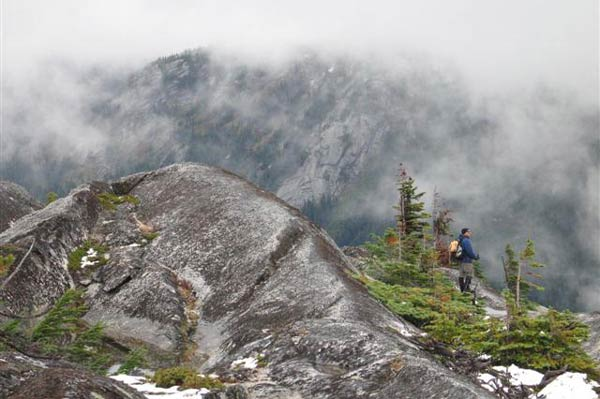
\includegraphics[scale=0.4]{bilder/hiking.jpg} & 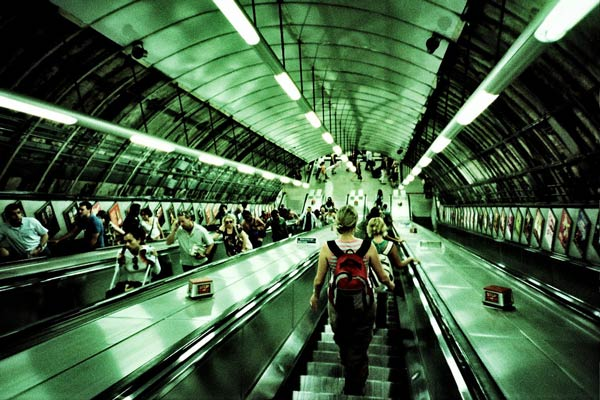
\includegraphics[scale=0.4]{bilder/tube.jpg}\\
			\multicolumn{2}{c}{
				\ccLogo\ 
				\begingroup
    				\fontsize{8pt}{12pt}\selectfont
    				\href{http://hood.ie/}{Hoodie Open Source Project}; Lizenz: \href{http://creativecommons.org/licenses/by-nc-nd/4.0/deed.en}{CC BY-NC-ND 4.0} 
				\endgroup
			}
		\end{tabulary}
  		\end{adjustwidth}
	\end{table}

%\\ \\
\noindent
Letztendlich wird die Möglichkeit zur Verbindungs-unabhängigen Realisierung einer Funktion durch ihren Zweck bedingt. Eine Navigations-Hilfe sollte den Benutzer in Echtzeit über eine zu wählende Abzweigung informieren, während Kommunikation zwischen Benutzern nicht nur über Telefonie oder Instant-Messaging, sondern häufig auch per Email noch sinnvoll sein kann.\\ \\
%Für synchrone Interaktion zwischen Benutzern ist ja ein ursprüngliche Ziel der Vernetzung. Bei der Entwicklung der Anforderungen kann aber berücksichtigt werden, daß auch für synchrone Interaktions-Funktionalität, wie beispielsweise Instant-Messaging, eine optionale asynchrone Alternative in Form einer verzögerten Nachrichten-Übermittlung, immer noch den zugedachten Zweck erfüllen kann.\\ \\
\noindent
Im Rahmen dieser Arbeit soll nun eine Web-Awendung für kollaboratives Geo-Tagging$^{\textbf{\ref{GEOTAG}}}$%
% footnote
\addtocounter{footnote}{1}%
\footnotetext{\label{GEOTAG}Geo-Tagging bedeutet die Referenz von Informationen zu einem Ort und wird in Abschnitt \ref{sec:GL:GEOTAG} erläutert.}
entwickelt werden. Die Anwendungs-Funktionen sollen dabei weitestgehend sowohl im Multi-User-Online-Modus wie auch im Single-User-Offline-Modus verfügbar sein.
%Ergebnisse von Verbindungs-abhängigen Aktionen, die im Offline-Modus ausgeführt wurden, werden bei wieder hergestellter Netzwerk-Verbindung mit dem System synchronisiert.
% In Abschnitt \ref{2_VOYAGEX} folgt eine Beschreibung der gewünschten Funktionen. 

%%%%%%%%%%%%%%%%%%%%%%%%%%%%%%%%%%%%%%%%%%%%%%%%%%%%%%%%%%%%%%
% Aufbau der Arbeit / Gliederung
%%%%%%%%%%%%%%%%%%%%%%%%%%%%%%%%%%%%%%%%%%%%%%%%%%%%%%%%%%%%%%
\subsection{Aufbau der Arbeit / Gliederung}
\subparagraph{Kapitel 2}
In diesem Kapitel werden zunächst 2 Szenarien zur Entwicklung und zum Einsatz einer Geo-basierten und kooperativen (mobilen) Anwendung beschrieben, und anschließend die Problematik Netzwerk-Verbindungs-abhängiger Funktionalität
konkret in Bezug auf die Funktionen kooperatives Geo-Tagging und Echtzeit-Kommunikation
analysiert.
%In diesem Kapitel werden Anwendungsfälle und Szenarien, sowie grundlegende Begriffe aus dem Bereich der Geo-Informations-Systeme und den darin verwendeten Datenmodellen und Werkzeugen beschrieben. Außerdem werden Prinzipien und Muster für Anwendungs-Systeme aus diesem Bereich vorgestellt. 

\subparagraph{Kapitel 3}
%Die Basis-Funktionen der in dieser Arbeit entwickelten Anwendung sind also Geo-Tagging und Kommunikation.
Die in Kapitel 2 analysierten Funktionen sind jeweils auch Kern-Funktionen von 2 sehr verbreiteten Anwendungsbereichen: \texttt{ortsbezogene Dienste (Location Based Services / LBS)} und \texttt{soziale Netzwerke (Social Networks / SN)}. Durch ihr synergetisches Potential werden diese Bereiche in vielen Anwendungen als \texttt{Location Based Social Networks (LBSN)} zusammengeführt. Auch die in dieser Arbeit vorgestellte Anwendung kann als LBSN-Anwendung klassifiziert werden, Grund genug, diese Anwendungs-Domäne etwas genauer zu untersuchen.\\ \\
In diesem Kapitel werden Grundlagen aus
%dem Bereich der Geo-Informations-Systeme
dem Anwendungs-Bereich sowie die darin verwendeten Datenmodelle und Werkzeuge beschrieben.
%Außerdem werden Prinzipien und Muster für Anwendungs-Systeme aus diesem Bereich vorgestellt. 
Anschließend werden historische und aktuelle Projekte und Anwendungen vorgestellt, und
deren Funktionaliät untersucht.

%\subparagraph{Kapitel 4}
%In diesem Kapitel wird die aus den Untersuchungen des vorigen Kapitels abgeleitete gewünschte Funktionalität %für VoyageX in Form von Use-Cases festgelegt, und der konzeptionelle Rahmen festgelegt.

\subparagraph{Kapitel 4}
In diesem Kapitel wird die technische Planung und Umsetzung dokumentiert. Dazu werden die System-Komponenten  sowie die technischen Voraussetzungen für die Laufzeit-Umgebung definiert.\\
Die für die Realisierung verwendeten Standards, Bibliotheken und 3$^{rd}$-Party Tools werden vorgestellt, wie auch die Algorithmen und erforderlichen Funktionalitäten zur Implementierung der Anforderungen.

\subparagraph{Kapitel 5}
Im letzten Kapitel wird der Nutzen der Anwendung noch einmal im Kontext der Anwendungs-Domäne beschrieben, sowie Möglichkeiten zur Weiterentwicklung bzw. zur Integration der Module in eine existierende Anwendung aufgezeigt.



\newpage
%%%%%%%%%%%%%%%%%%%%%%%%%%%%%%%%%%%%%%%%%%%%%%%%%%%%%%%%%%%%%%
%
% Kapitel 2: Szenarien und Anwendungsfälle
%
%%%%%%%%%%%%%%%%%%%%%%%%%%%%%%%%%%%%%%%%%%%%%%%%%%%%%%%%%%%%%%
\section{Problemstellung}
Im folgenden ersten Kapitel wird zunächst in Abschnitt \ref{2_SZEN} das Problem zur Entwicklung einer Geo-Taggingg$^{\textbf{\ref{GEOTAG}}}$-Anwendung in Form einer Beschreibung von konkreten und fiktiven Szenarien gestellt. Anschließend wird in Abschnitt \ref{2_VOYAGEX} die in dieser Bachelor-Arbeit entwickelte Anwendung \textbf{VoyageX} vorgestellt.
% und ihre Funktionen beschrieben.
%widmet sich den Grundlagen des Anwendungs-Bereichs von Geo-Informations-Systemen (GIS). Gleichwohl
%scheint eine einführende Beschreibung in Abschnitt \ref{2_VOYAGEX} der im Rahmen dieser Arbeit entwickelten %Anwendung sinnvoll, um von Beginn an einen praktischen Rahmen für die folgenden Abschnitte herzustellen.
%In Abschnitt \ref{2_GRUNDL} werden Begriffe eingeführt und historische Entwicklungen beschrieben.
%In Abschnitt \ref{2_LBSN} werden Konzepte und Entwicklung Aufenthalts-basierter sozialer Netzwerke beschrieben, durch welche, aufgrund von Benutzerzahlen im über 7-stelligen Bereich, die Entwicklung Standort-bezogener Anwendungen einen Quantensprung vollführte.


%%%%%%%%%%%%%%%%%%%%%%%%%%%%%%%%%%%%%%%%%%%%%%%%%%%%%%%%%%%%%%
% Szenario
%%%%%%%%%%%%%%%%%%%%%%%%%%%%%%%%%%%%%%%%%%%%%%%%%%%%%%%%%%%%%%
\subsection{Szenario}\label{2_SZEN}
Im Rahmen des Projekts \textbf{Pumas Voyage}$^{\textbf{\ref{CMTPUMVOY}}}$%
% footnote
\addtocounter{footnote}{1}%
\footnotetext{\label{CMTPUMVOY}\href{http://ceur-ws.org/Vol-1227/paper33.pdf}{Pumas Voyage - http://ceur-ws.org/Vol-1227/paper33.pdf}; letzter Zugriff: 26.04.2015} werden Konzepte und Werkzeuge für die Beteiligung von Schülern an der Verkehrsraumplanung entwickelt. Die Schüler sollen dabei, mit Hilfe von mobilen Endgeräten und einer darauf ausgeführten Web-Anwendung, ihren Schulweg durch Einträge von markanten Punkten  auf einer Karte mit einer Bewertung von Sicher/Gut oder Gefährlich/Schlecht, und einem optionalen Kommentar, dokumentieren$^{\textbf{\ref{CMTPUMVOYGEOTAG}}}$
% footnote
\addtocounter{footnote}{1}%
\footnotetext{\label{CMTPUMVOYGEOTAG}Man könnte diesen Vorgang auch als Verkehrsplanungs-spezifisches Geo-Tagging bezeichnen}.\\
Für die Anwendung gelten folgende Einschränkungen:
\begin{itemize}[leftmargin=*,noitemsep,topsep=1ex,parsep=0pt,partopsep=0pt]
\item Eine Voraussetzung für die Bearbeitung von PoI-Einträgen ist die Anzeige einer Karte in der Anwendungs-Oberfläche. Für die Bereitstellung der dazu benötigten Bild-Dateien ist eine Internet-Verbindung erforderlich.
\item Ein Austausch der PoI-Daten mit anderen Benutzern ist nicht möglich - auf jedem Gerät können nur die darauf (lokal) gesicherten Daten angezeigt werden.
\end{itemize}
\vspace{1ex}
Eine Netzwerk-Verbindungs-unabhängige Möglichkeit der Karten-Anzeige würde es den Benutzern erlauben, auch im Offline-Modus mit der Anwendung zu arbeiten.\\ \\
Die Synchronisation aller Benutzer/System-Daten und deren Anzeige auf allen Endgeräten würde die Anwendung um kollaborative Funktionalität erweitern, mit der es zum Beispiel die Möglichkeit zum zeitversetzten oder auch unmittelbaren Feedback auf neue Einträge oder Änderungen gäbe.
%Damit aber keine Netzwerk-Verbindungs-Abhängigkeit entsteht sollte die
%Diese Synchronisation sollte für den Benutzer transparent durchgeführt werden.\\ \\
\noindent
Neben dem bereits realisierten Szenario des Pumas-Voyage Projekts soll im folgenden auch ein fiktives Szenario für eine andere Anwendungsnutzer-Gruppe beschrieben werden:\\ \\
Petra lebt in Berlin. Sie ist eine große Bewunderin von Street-Art und fährt in ihrer Freizeit gerne mit dem Fahrrad durch die Stadt um neue Werke zu entdecken und zu Fotografieren. Sie nutzt die VoyageX-Webapp um ein neu entdecktes Plakat von El Bocho$^{\textbf{\ref{CMTELBOC}}}$%
% footnote
\addtocounter{footnote}{1}%
\footnotetext{\label{CMTELBOC}\href{http://www.elbocho.net/}{El Bocho - http://www.elbocho.net/} (letzter Zugriff: 30.04.2015)} oder ein neues Street-Yogi-Korkmännchen$^{\textbf{\ref{CMTJOYFOX}}}$%
% footnote
\addtocounter{footnote}{1}%
\footnotetext{\label{CMTJOYFOX}\href{http://de.wikipedia.org/wiki/Korkm\%C3\%A4nnchen}{Korkmännchen - http://de.wikipedia.org/wiki/Korkm\%C3\%A4nnchen} (letzter Zugriff: 30.04.2015)} von Joy Fox zu speichern, und mit Freunden oder Gleichgesinnten zu teilen.
\\ %Einmal im Jahr fährt sie für 3 wochen nach Südost-Asien in den Urlaub, \\
Markus kommt ursprünglich auch aus Berlin, wohnt aber jetzt berufsbedingt in Neuruppin. Auch er interessiert sich für Street-Art. Petra und Markus kennen sich über Facebook, wo beide früher ihre Fotos gepostet haben. Er fährt mindestens 2 mal in der Woche nach Berlin. In der Stadt benutzt er meistens die öffentlichen Verkehrsmittel.\\ \\
Seit seinem letzten Berlin-Besuch haben andere User neue Fundstücke in VoyageX eingetragen, und Markus möchte diese in natura sehen, bevor sie übermalt werden oder auf andere Weise verloren gehen. Zuhause hat er in VoyageX Lesezeichen für die PoIs erstellt, die er sich ansehen möchte, und auch die geplante Route für seine Besichtigungstour gespeichert. Auf der 1-stündigen Zugfahrt kommt er mit Klaus, einem Mitreisenden aus Wittstock, ins Gespräch. Als Markus ihm über das Motiv seiner Reise erzählt, würde Klaus gerne mal Fotos dieser Straßen-Kunst sehen. Von der unterbrochenen Internetverbindung im Zug merken die beiden nichts während Markus seine Fotos in VoyageX zeigt.\\ \\
In Berlin angekommen beginnt Markus seine Tour. Gleich beim ersten PoI entdeckt er neben dem bereits eingetragenen Werk ein neues Street-Art-Fundstück und postet es als Kommentar mit Foto.\\
Zum nächsten PoI nimmt er die U-Bahn. In einer Umstiegs-Station entdeckt er ein neues Poster von einer ihm unbekannten Künstlerin. Er macht ein Foto und möchte es mit einem neuen PoI speichern. Da in der U-Bahn aber keine GPS-Ortung möglich ist, muss Markus die Position auf der Karte manuell markieren. Obwohl auch keine Mobil-Funk-Netzverbindung verfügbar ist, kann er zum Kartenauschnitt für seinen aktuellen Standort zoomen und die PoI-Markierung setzen. VoyageX hat die benötigten Karten-Bild-Dateien (vor)geladen als er noch zu Fuß unterwegs zur U-Bahn-Station war. Der Eintrag wird aber vom VoyageX-Client erst dann zum Server gepostet (und damit für die anderen VoyageX-User sichtbar sein), wenn Markus das U-Bahn-System wieder verlässt und wieder Funk-Netz-Zugang hat.\\
Als er (mittlerweile wieder oberirdisch) auf dem Weg zum nächsten PoI ist, wird er durch ein akkustisches Signal und einen blinkenden Pfeil in VoyageX darauf aufmerksam gemacht, daß einer seiner Kontakte in der Nähe ist. Es ist Petra, die beiden verabreden sich in einem Kaffee. Nachdem Petra auch Markus auf ihrer Karte "`ortet"', kann sie ihm eine Wegbeschreibung senden, in dem sie den Weg auf seiner Karte "`zeichnet"'.
%wegvorhersage noch gar nicht drinn mit dem u-bahn verbinden ?
Beim Kaffee kann sie ihm dann auch noch verraten, wer die Künstlerin seines U-Bahn-Fundstückes ist, aber als er seinem VoyageX-Eintrag den Namen hinzufügen will, stellt er fest, daß ihm ein anderer VoyageX-User bereits zuvorgekommen ist.%\\
%Als Markus im Zug nach Hause sitzt möchte er sich nochmal die Bilder ansehen, die er im Anschluss an das Treffen noch gespeichert hat. Ihm fällt dabei gar nicht auf, daß VoyageX auch die Bilddateien für die Kartenauschnitte automatisch gespeichert hat, und so merkt er auch nicht wenn die Mobil-Funk-Verbindung im Zug schon wieder unterbrochen ist.%\\
%	\begin{table}[H]
%  		\begin{adjustwidth}{-1cm}{1cm}
%		\centering
%		\begin{tabulary}{15cm}{C >{\centering}m{1cm} C >{\centering}m{1cm} C}
%			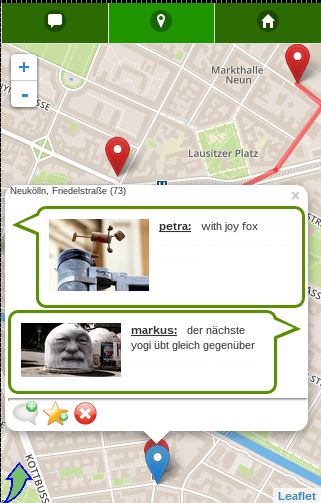
\includegraphics[scale=0.6]{bilder/joy-fox-2.png} & & 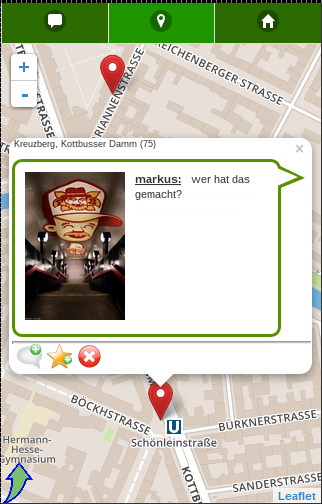
\includegraphics[scale=0.6]{bilder/wer-war-das} & & 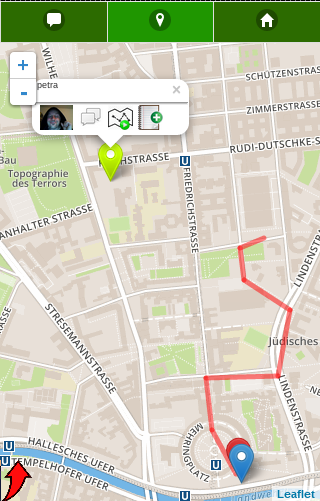
\includegraphics[scale=0.6]{bilder/petra-alert.png}
%		\end{tabulary}
%  		\end{adjustwidth}
%	\end{table}
%asien - überöandbus - nur wlsan - keine sim
%kaum zu glauben - sie seiht das ien freun din der nähe ist

%er bookmared alöe die ers sehen will
%dann shauut er
%irgedwann sieht er das petra in der nähe ist
%er fragt wo sie sih treffen und wie er mal besten hin komt

%offlien im zug nachhause macht er neue kommentare mit wietern fotos einträge mit ofotos.  (mnahce fotso 

%als er zu hause ankommt kriegt er nahcrichten von ein paat lezten oder am nächsten morgen wacht er auf

%Als er zu Hause die Bilder auf seinem Smartphone betrachtet schreibt er \\ \\
%\noindent
%Seit der Einführung des AppCache-Standards in Html5 
% Seit Ende der 2000-nuller Jahre
%\noindent
%\textbf{Ingress}$^{\textbf{\ref{CMTINGRS}}}$%
% footnote
%\addtocounter{footnote}{1}%
%\footnotetext{\label{CMTINGRS}\href{http://de.wikipedia.org/wiki/Ingress\_\%28Spiel\%29}{Ingress - http://de.wikipedia.org/wiki/Ingress\_\%28Spiel\%29}; letzter Zugriff: 26.04.2015} ist ein Augmented-Reality-/Alternate-Reality-Spiel für mobile Geräte. Das Spiel wird im Freien gespielt, und die Spielwelt wird mit standortbezogenen Daten von realen sich an Gebäuden, Denkmälern und Objekten aufgebaut. Im Spiel existieren zwei Gruppierungen, die mit dem Ziel gegeneinander antreten, möglichst große öffentliche Bereiche unter ihre virtuelle Kontrolle zu bringen.\\ \\
%\noindent


%synchron bearbeitung von pois.
%man sieht gkeuch den pi
%man kann auch auf anderen zeichnen 
%spiele, navi 

%%%%%%%%%%%%%%%%%%%%%%%%%%%%%%%%%%%%%%%%%%%%%%%%%%%%%%%%%%%%%%
% Analyse
%%%%%%%%%%%%%%%%%%%%%%%%%%%%%%%%%%%%%%%%%%%%%%%%%%%%%%%%%%%%%%
\subsection{Analyse}\label{2_VOYAGEX}
%\subsubsection{Client und Benutzer/User}
%Vorab noch Definitionen zweier in dieser Arbeit sehr häufig verwendete Begriffe:   
%\begin{itemize}
%	\item \textbf{Client}: Eine Anwendungs-Komponente des Frontends, je nach Kontext ist damit entweder der Browser oder der VoyageX-Client gemeint. 
%	\item \textbf{Benutzer / User}: Eine Person, welche die Anwendung (insbesondere den Client) nutzt.
%\end{itemize}
%\vspace{2ex}
Aus dem fiktiven Szenario können folgende 2 autonomen$^{\textbf{\ref{CMTAUTOGF}}}$%
% footnote
\addtocounter{footnote}{1}%
\footnotetext{\label{CMTAUTOGF}Jede einzelne dieser Funktionen kann für sich schon als (ggf. einzige) Kernfunktion einer Anwendung dienen.} Basis-Funktionen
%abgeleitet
extrahiert
werden:
\enlargethispage{3\baselineskip} % allow 3 more lines on current page
\begin{itemize}[leftmargin=*,noitemsep,topsep=1ex,parsep=0pt,partopsep=0pt]
\item \textbf{Geo-Tagging}$^{\textbf{\ref{GEOTAG}}}$: Einträge für \texttt{Points of Interest (PoI)} erstellen
\item \textbf{Informale Kommunikation}: Nachrichtenaustausch zwischen Benutzern
\end{itemize}
Diese Funktionen werden nun durch Basiskonzepte kooperativer Systeme\cite{K1678:VERTSYS} (S.180-182) um eine kollaborative Dimension erweitert und wir spezifizieren:
\begin{itemize}[leftmargin=*,noitemsep,topsep=1ex,parsep=0pt,partopsep=0pt]
\item \textbf{Gemeinsame Objekte}: Alle Benutzer können die PoIs sehen und weitere Informationen hinzufügen. Dies entspricht auch einer impliziten formalen Kommunikation.
\item \textbf{explizite formale Kommunikation}: Message Passing und Remote Procedure Calls (RPC)
\end{itemize}
Abschließend wird noch eine Verbindungs-Zustands-bezogene Dimension eingeführt:
\begin{itemize}[leftmargin=*,noitemsep,topsep=1ex,parsep=0pt,partopsep=0pt]
\item \textbf{online}: Uneingeschränkte Nutzung aller Funktionen
\item \textbf{offline}: Nutzung möglichst aller Funktionen unter eventuell erforderlicher Anpassung des Funktions-Verhaltens
\end{itemize}
\vspace{1ex}\noindent
Nach dieser Analyse der gewünschten Funktionen können wir die geplante Anwendung als "`kooperatives Netzwerk-Verbindungs-unabhängiges System"' mit 2 Basis-Funktionen beschreiben, wobei die Basis-Funktionen austauschbar sind.\\ \\
% und für eine weitere Klassifikation keine Rolle spielen.\\ \\
Kooperative Systeme können nach Grudin\cite{GRUDIN:CSCW} (S.19-26) mit einer Raum-Zeit-Matrix klassifiziert werden. Die räumliche Dimension ist für die hier zu entwickelnde (mobile) Anwendung festgelegt: Orte werden als \texttt{verschieden} und \texttt{unvorhersehbar} vorausgesetzt, zeitlich kann aber in eine \texttt{synchrone} und eine \texttt{asynchrone} Kooperation differenziert werden. Zusammen mit dem Netzwerk-Verbindungs-Status lassen sich nun für die beiden Basis-Funktionen jeweils folgende Anwendungs-Dimensionen eingrenzen:\\
%Die in den zuvor beschriebenen Szenarien benötigten Anwendungsfunktionen können wie folgt eingeteilt werden:
%\begin{itemize}[leftmargin=*,noitemsep,topsep=1ex,parsep=0pt,partopsep=0pt]
%\item \textbf{Geo-Tagging}: Einträge für \texttt{Points of Interest (PoI)} erstellen
%\item \textbf{verbindungsunabhängig}: Benutzbarkeit der Anwendung auch im offline-Modus
%\item \textbf{kollaborativ}: Interaktion durch Kooperation und Kommunikation
%\begin{itemize}[noitemsep,topsep=0ex,parsep=0pt,partopsep=0pt]
%\item Gemeinsame Objekte: Alle Benutzer können die PoIs sehen und weitere Informationen hinzufügen.
%\item Austausch von Nachrichten: Benutzer können mittels Chat-Nachrichten kommunizieren.
%\end{itemize}
%\end{itemize}
%Geo-Tagging ist 
%Mit der in dieser Arbeit vorgestellten Web-Anwendung VoyageX sollen nun folgende Funktionen implementiert %werden:
\enlargethispage{3\baselineskip} % allow 3 more lines on current page
\newcolumntype{M}{>{\raggedright\arraybackslash}p{7.5cm}}
%\begin{itemize}
%  \item Kollaborative Bearbeitung von Points of Interest (PoI) auf einer interaktiven Karte
\subparagraph{Kooperative Bearbeitung von PoIs:}
	\begin{table}[H]
  		\begin{adjustwidth}{-1.7cm}{1.7cm}
		\centering
		\begin{tabulary}{19cm}{|C|M|M|}
		%\begin{tabulary}{\columnwidth}{|C|L|L|}
			\hline
		  & \multicolumn{1}{c|}{online} & \multicolumn{1}{c|}{offline} \\ \hline
synchron &
%%Neu erstellte Einträge/Kommentare und Änderungen werden unmittelbar auf allen online-Clients angezeigt.
				\begingroup
    				\fontsize{9pt}{10pt}\selectfont
%\textbf{Benachrichtigungen bei Daten-Änderungen durch entfernte Benutzer}:\newline
%\ref{2_POISYNCONL}
%Für eine kollaborative Anwendung gelten folgende Anforderungen: 
\begin{itemize}[leftmargin=*,noitemsep,topsep=0ex,parsep=1pt,partopsep=0pt]
	\item Neu erstellte Einträge und Änderungen werden unmittelbar
		  auf allen online-Clients angezeigt
	%\item Von einem Benutzer lokal neu erstellte Einträge/Kommentare und Änderungen werden unmittelbar auf entfernten online-Clients angezeigt
\end{itemize}
%In der Praxis werden nur relevante Einträge auf jedem Client gespeichert, wobei sich die Relevanz auf geographische Nähe oder die Autorenschaft des Eintrags (z.B. von einer Freundin) gründet.
				\endgroup
&
%%Neu erstellte Einträge/Kommentare und Änderungen werden in einer lokalen Warteschlange gespeichert und angezeigt.
				\begingroup
    				\fontsize{9pt}{10pt}\selectfont
%\textbf{Vorhalten existierender, und Speichern neuer Anwendungs-Daten}:\newline
%\ref{2_POISYNCOFFL}
%Damit die Nutzung der Anwendung auch im Offline-Modus möglich bleibt, müssen folgende Anforderungen erfüllt werden:
%\begin{itemize}[leftmargin=*,noitemsep,topsep=0ex,parsep=1pt,partopsep=0pt]
%	\item Anwendungs-Daten (Poi-Einträge, Karten-Kachel-Bilder) werden aus dem lokalen Speicher gelesen
%	\item Neu erstellte Einträge/Kommentare und Änderungen werden lokal gespeichert
%\end{itemize}
\begin{itemize}[leftmargin=*,noitemsep,topsep=0ex,parsep=1pt,partopsep=0pt]
	\item Erstellen neuer Einträge
	\item Bearbeiten eigener Einträge
\end{itemize}
				\endgroup
\\ \hline
asynchron &
%Beim Wechsel vom Offline- in den Online-Modus werden die lokalen Daten mit den System-Daten synchronisiert:\newline
%			- die Daten aus der lokalen Warteschlange werden in die Backend-DB überspielt und alle online-Clients werden benachrichtigt\newline
%			- Änderungen im Backend werden in die lokale DB eingespielt
				\begingroup
    				\fontsize{9pt}{10pt}\selectfont
%\textbf{Synchronisation von Daten-Änderungen}:\newline
% \ref{2_POIASYNCONL}
Beim Wechsel vom Offline- in den Online-Modus werden die lokalen Daten mit den System-Daten synchronisiert:
\begin{itemize}[leftmargin=*,noitemsep,topsep=1ex,parsep=0pt,partopsep=0pt]
	\item lokale Änderungen werden in die Backend-DB überspielt und alle online-Clients werden benachrichtigt
	\item Änderungen in der Backend-DB werden in die lokale DB eingespielt
\end{itemize}
				\endgroup
		& %\multicolumn{1}{c|}{-}
				\begingroup
    				\fontsize{9pt}{10pt}\selectfont
\begin{itemize}[leftmargin=*,noitemsep,topsep=1ex,parsep=0pt,partopsep=0pt]
    \item Bearbeiten von Einträgen entfernter Benutzer
\end{itemize}
				\endgroup
		\\ \hline
		\end{tabulary}
  		\end{adjustwidth}
	\end{table}
%  \item Interaktion: Benutzer-Benutzer und System-Benutzer
\vspace{1ex}\noindent
\subparagraph{Interaktion: Benutzer-Benutzer und System-Benutzer:}
	\begin{table}[H]
  		\begin{adjustwidth}{-1.7cm}{1.7cm}
		\centering
		\begin{tabulary}{18cm}{|C|M|M|}
		%\begin{tabulary}{\columnwidth}{|C|L|L|}
			\hline
		  & \multicolumn{1}{c|}{online} & \multicolumn{1}{c|}{offline} \\ \hline
synchron  & 
				\begingroup
    				\fontsize{9pt}{10pt}\selectfont
%\textbf{Echtzeit-Interaktion}:\newline
%\ref{2_ISYNCONL}
%- Benutzer können Chat-Nachrichten austauschen\newline
%			- Benutzer können auf dem lokalen Client aktuelle Standorte anderer Benutzer sehen\newline
%			- Benutzer können GUI-Objekte auf einem entfernten Client steuern
\begin{itemize}[leftmargin=*,noitemsep,topsep=1ex,parsep=0pt,partopsep=0pt]
	\item Benutzer können Kontakt-Verbindungen eingehen und diese bearbeiten
	\item Benutzer können Chat-Nachrichten austauschen
	\item Benutzer können auf dem lokalen Client aktuelle Standorte anderer Benutzer sehen
	\item Benutzer können GUI-Objekte auf einem entfernten Client steuern
\end{itemize}
				\endgroup
& 
				\begingroup
    				\fontsize{9pt}{10pt}\selectfont
%\textbf{Verzögerte Kommunikation}:\newline
%\ref{2_ISYNCOFFL}
%Neu erstellte Chat-Nachrichten werden lokal in einer Warteschlange gespeichert und angezeigt.
%Im Idealfall können auch alle Aktionen der Kontaktverwaltung im offline-Modus ausgeführt werden. Allerdings wird dies eventuell in VoyageX noch nicht implementiert.
\begin{itemize}[leftmargin=*,noitemsep,topsep=1ex,parsep=0pt,partopsep=0pt]
	\item Neu erstellte Chat-Nachrichten werden lokal in einer Warteschlange gespeichert
\end{itemize}
				\endgroup
\\ \hline
asynchron &
				\begingroup
    				\fontsize{9pt}{10pt}\selectfont
%\textbf{Synchronisation von Kommunikations-Daten}:\newline
%\ref{2_IASYNCONL}
%Beim Wechsel vom Offline- in den Online-Modus werden:\newline
%- Nachrichten aus der lokalen Warteschlange an die Adressaten versendet\newline
%- Nachrichten an den lokalen Benutzer aus einer Backend-Warteschlange empfangen
Beim Wechsel vom Offline- in den Online-Modus werden die lokalen Daten mit den System-Daten synchronisiert:
\begin{itemize}[leftmargin=*,noitemsep,topsep=1ex,parsep=0pt,partopsep=0pt]
	\item Nachrichten aus der lokalen Warteschlange an die online-Adressaten versendet
	\item Nachrichten an den lokalen Benutzer aus einer Backend-Warteschlange empfangen
\end{itemize}
				\endgroup
&% \multicolumn{1}{c|}{-}  
				\begingroup
    				\fontsize{9pt}{10pt}\selectfont
\begin{itemize}[leftmargin=*,noitemsep,topsep=1ex,parsep=0pt,partopsep=0pt]
	\item Nachrichten die an den lokalen Benutzer gesendet werden während er sich im offline-Modus befindet, werden im Backend gespeichert
\end{itemize}
				\endgroup
\\ \hline
		\end{tabulary}
  		\end{adjustwidth}
	\end{table}
%\end{itemize}
%Im folgenden werden also auch die Konzepte und Funktionalität dieser Komponenten vorgestellt.
%Mitwirkende Benutzer müssen sich auf der Web-Seite registrieren um die Bearbeitungs-Funktionen nutzen zu können. Nicht
%registrierte Benutzer können nur "`lesend"' auf die Anwendung zugreifen.\\ \\
%\subsection{Funktionsumfang}\label{4_FU}
%\begin{itemize}[leftmargin=*,noitemsep,topsep=1ex,parsep=0pt,partopsep=0pt]
%\item \textbf{plain text}: ein plain-text eintrag besteht nur aus text. allerdings wird als default icion ein %\end{itemize}
%\subsubsection{Darstellung der Karte und positionsbezogener Gestaltungs-Elemente}
\vspace{2ex}
\enlargethispage{3\baselineskip} % allow 3 more lines on current page
\noindent
Eine Entkopplung von der Netzwerk-Verbindungs-Abhängigkeit muß also durch die Möglichkeit zum lokalen Speichern von Anwendungs-Daten, sowie durch das Vorhalten der für die Nutzung der Software benötigten System-Daten bewerkstelligt werden. Allerdings können aus Gründen der Wartbarkeit und der begrenzten Speicher-Kapazität nicht alle System-Daten auf einem Endgerät gespeichert werden. Es ist daher erforderlich, eine Auswahl bezüglich der vom Benutzer benötigten Daten zu treffen und diese vorzuhalten - im Falle einer kartenbasierten Anwendung müssen dafür beispielsweise die Bild-Dateien für die darzustellenden Karten-Abschnitte vorgeladen werden. Die Vorlade-Auswahl kann mit Hife von aufgabenspezifischen Vorhersage-Algorithmen getroffen werden. Im gegebenen geographischen Kontext können die Vorhersage-Strategien beispielsweise auf Bewegungs-Routen basieren. 


\newpage
%%%%%%%%%%%%%%%%%%%%%%%%%%%%%%%%%%%%%%%%%%%%%%%%%%%%%%%%%%%%%%
%
% Kapitel 3: Existierende Lösungen
%
%%%%%%%%%%%%%%%%%%%%%%%%%%%%%%%%%%%%%%%%%%%%%%%%%%%%%%%%%%%%%%
%\enlargethispage{3\baselineskip} 
\section{Grundlagen und Existierende Lösungen}
Nach einem Überblick über Grundlagen und Entwicklung ortsbezogener Anwendungen in den Abschnitten \ref{3_GRUNDL} und \ref{3_LBS_HIST} werden 5 existierende Anwendungen beschrieben und ausgewählte Funktionen zusammen mit Funktionen von VoyageX untereinander verglichen (Abschnitt \ref{3_ANW}). Das Kapitel schliesst mit einer Zusammenstellung weit verbreiteter, von den meisten Anwendungen genutzter externer Dienste%
%von Dritten
, den Web Mapping APIs (Abschnitt \ref{3_WEBMAPAPIS}).

%%%%%%%%%%%%%%%%%%%%%%%%%%%%%%%%%%%%%%%%%%%%%%%%%%%%%%%%%%%%%%
% Grundlagen
%%%%%%%%%%%%%%%%%%%%%%%%%%%%%%%%%%%%%%%%%%%%%%%%%%%%%%%%%%%%%%
\subsection{Grundlagen ortsbezogener Anwendungen}\label{3_GRUNDL}
Seit der Entwicklung des ersten personalisierten Lokalisierungssystems$^{\textbf{\ref{ATTACTBADG}}}$%
% footnote
\addtocounter{footnote}{1}%
\footnotetext{\label{ATTACTBADG}\href{http://www.cl.cam.ac.uk/research/dtg/attarchive/ab.html}{Active Badge System - http://www.cl.cam.ac.uk/research/dtg/attarchive/ab.html}; letzter Zugriff: 23.04.2015}
anfangs der 1990er haben Verbreitung und Reichweite von Endgeräten mit der Fähigkeit zur Positions-Bestimmung in Form von Smartphones eine nahezu ubiquitäre Dimension erreicht. Für die Benutzer eines solchen Geräts ist es möglich, anderen Menschen den eigenen aktuellen geographischen Standort mitzuteilen. \\ \\
% reicht der , und Objekte oder sogar Personen anhand ihre Positions-Daten identifizieren. \\ \\
Seit Anfang 2000 (siehe Tabelle \ref{LBSHISTORYTABLE}) ist vor diesem Hintergrund eine Vielzahl von Anwendungen mit einer Einbindung "`Standort-bezogener Dienste"' entwickelt worden. Die Möglichkeit einer Anzeige von Informationen zu Markierungs-Punkten auf einer Karte kann in vielerlei Hinsicht genutzt werden, unter anderem für:
\begin{itemize}
  \item Geo-Tagging$^{\textbf{\ref{GEOTAG}}}$ von Orten / Objekten (Points of Interest) und Ereignissen (Events of Interest)
  \item zeitbezogene Lokalisierung von Personen (People of Interest) und Ereignissen
\end{itemize}
Für "`Points of Interest"' oder "`Events of Interest"' können die angezeigten Informationen neben einer objektiven Beschreibung auch subjektive Bewertungen oder Empfehlungen beinhalten, für "`People of Interest"' kann eine Möglichkeit zur direkten Kontaktaufnahme über einen Chat-Dialog verknüpft werden.\\ \\
Viele der aktuellen mobilen Anwendungen nutzen eigene Backends und freie Web-Services von Dritten als Geo-Informations-Quellen. Diese Clients werden vorwiegend als native Anwendungen über den App-Store$^{\textbf{\ref{CMTAPPST}}}$%
% footnote
\addtocounter{footnote}{1}%
\footnotetext{\label{CMTAPPST}\href{http://de.wikipedia.org/wiki/App\_Store\_\%28iOS\%29}{App-Store - http://de.wikipedia.org/wiki/App\_Store\_\%28iOS\%29}; letzter Zugriff: 23.04.2015} für iOS$^{\textbf{\ref{CMTIOS}}}$%
% footnote
\addtocounter{footnote}{1}%
\footnotetext{\label{CMTIOS}\href{http://de.wikipedia.org/wiki/Liste\_von\_iOS-Ger\%C3\%A4ten}{iOS - http://de.wikipedia.org/wiki/Liste\_von\_iOS-Ger\%C3\%A4ten}; letzter Zugriff: 23.04.2015} oder Google-Play$^{\textbf{\ref{CMTGOOPL}}}$%
% footnote
\addtocounter{footnote}{1}%
\footnotetext{\label{CMTGOOPL}\href{http://de.wikipedia.org/wiki/Google\_Play}{Google-Play - http://de.wikipedia.org/wiki/Google\_Play}; letzter Zugriff: 23.04.2015} für Android$^{\textbf{\ref{CMTANDROID}}}$%
% footnote
\addtocounter{footnote}{1}%
\footnotetext{\label{CMTANDROID}\href{http://de.wikipedia.org/wiki/Android\_\%28Betriebssystem\%29}{Android - http://de.wikipedia.org/wiki/Android\_\%28Betriebssystem\%29}; letzter Zugriff: 23.04.2015} angeboten.%\\
%Bearbeitung von Karteneinträgen im Offline-Modus wird nicht angeboten.

\subsubsection{Geo-Informations-Systeme und Kartendienste}
"`\textit{Ein Geo-Informations-System (GIS) ist ein System zur Erfassung, Speicherung,  Bearbeitung, Analyse, Organisation und Präsentation für jede Art von räumlicher oder geographischer Information.}"'\cite{WIKI:GIS} \\
GIS bilden mit ihren Funktionen, Daten und Modellen die Grundlage für die Erstellung von Kontext-bezogenen Karten.\\ \\ %Ein Anwendungsbeispiel ist die Anzeige von standortbezogenen "`Gelbe Seiten"'-Einträgen auf Webseiten.\\
Die verschiedenen GIS-Standards werden vom Open Geospatial Consortium$^{\textbf{\ref{CMTOGC}}}$%
% footnote
\addtocounter{footnote}{1}%
\footnotetext{\label{CMTOGC}\href{http://www.opengeospatial.org/}{OGC - http://www.opengeospatial.org/}; letzter Zugriff: 23.04.2015} (OGC) entwickelt, und ermöglichen die Realisierung von unterschiedlichen \texttt{GIS-Anwendungen}. Beispielsweise wird vom OGC das \texttt{Web Map Service (WMS)}-Protokoll definiert, welches einen Standard für Kartendienste zur Bereitstellung von geo-referenzierten Bildern im Internet beschreibt.
Diese Dienste werden nun von Anwendungen zur kontextspezifischen Weiterverabeitung der geographischen Basis-Daten genutzt, wie beispielsweise von \texttt{Web-Mapping}-Projekten Google$^{\textbf{\ref{WIKIGOOGMAP}}}$%
% footnote
\addtocounter{footnote}{1}%
\footnotetext{\label{WIKIGOOGMAP}\href{http://de.wikipedia.org/wiki/Google_Maps}{http://de.wikipedia.org/wiki/Google\_Maps}; letzter Zugriff: 26.02.2015}
, Bing$^{\textbf{\ref{WIKIBINGMAP}}}$%
% footnote
\addtocounter{footnote}{1}%
\footnotetext{\label{WIKIBINGMAP}\href{http://en.wikipedia.org/wiki/Bing_Maps}{http://en.wikipedia.org/wiki/Bing\_Maps}; letzter Zugriff: 26.02.2015}
oder OpenStreetMaps$^{\textbf{\ref{WIKIWEBMAP}}}$%
% footnote
\addtocounter{footnote}{1}%
\footnotetext{\label{WIKIWEBMAP}\href{http://en.wikipedia.org/wiki/Geographic_information_system\#Applications}{http://en.wikipedia.org/wiki/Geographic\_information\_system\#Applications}; letzter Zugriff: 26.02.2015}  
 (siehe Abschnitt \ref{3_WEBMAPAPIS}).
%\vspace{0.8cm}
%  \begin{figure}[H]
%      \centering
%	  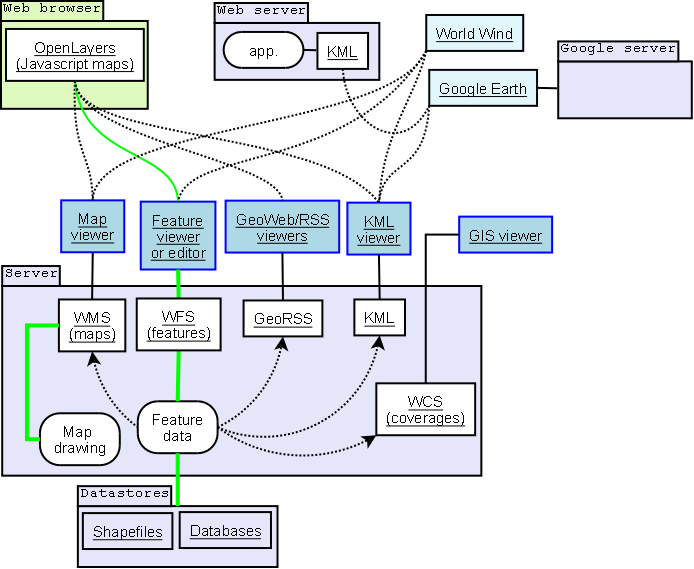
\includegraphics[scale=0.3]{bilder/Geoservices_server_with_apps.png}
%  	  \caption{
%  	  Vernetzung von GIS-Werkzeugen durch OGC Standards.\newline
%				\ccLogo\ 
%				\begingroup
%    				\fontsize{8pt}{12pt}\selectfont
%    				Quelle: wikipedia; Lizenz: \href{http://creativecommons.org/licenses/by-sa/3.0/}{CC BY-SA 3.0} 
%				\endgroup
%  	  }
%  \end{figure}

\subsection{Location Based Services (LBS)}\label{3_LBS_HIST}
\subsubsection{Geschichte}
In den 1990ern wurde mit dem Active Badge System$^{\textbf{\ref{ATTACTBADG}}}$ das erste Endgerät zur personellen Lokalisierung entwickelt.
Im folgenden wurden durch die Integration von Positions-Bestimmungs-Systemen in die zunehmend verbreiteten Mobil-Funk-Geräte die technischen Voraussetzungen für die Entwicklung von Anwendungen im Kontext Standort-bezogener Dienste für einen Massen-Markt geschaffen.\\
Wie bei vielen sozio-technischen Entwicklungen konnten hier Bereiche verschiedener existierender Anwendungs-Domänen aus der Sozial-Theorie und der Informations-Technologie verbunden, und zu eigenständigen neuen Anwendungs-Domänen weiterentwickelt werden.
%\subsubsection{Anwendungsbereiche}\label{sec:GL:GEOTAG}
%Ein naheliegendes Anwendungsgebiet für eine verbreitete Nutzung von LBS sind offensichtlich Kartendienste oder Webseiten und Anwendungen aus dem Bereich Tourismus. Die rein sachlichen Informationen zu geographischen Punkten werden hierbei oft auch mit subjektive Erfahrungsberichten ergänzt.\\
%, aus denen auch Crowd-Based-Recommender-System aufgebaut werden kann.\\
%Auf die Nutzung von LBS in Sozialen Netzwerke wird in Abschnitt \ref{2_LBSN} näher eingegangen.\\
%Geo-basierte Dienste werden auch von Spiele-Web-Seiten und Apps genutzt, wobei in der Regel auch eine %soziale Community um das Spiel entsteht. Als Beispiel sei hier Ingress$^{\textbf{\ref{WIKIINGRESS}}}$%
% footnote
%\addtocounter{footnote}{1}%
%\footnotetext{\label{WIKIINGRESS}\href{http://de.wikipedia.org/wiki/Ingress_(Spiel)}{http://de.wikipedia.org/wiki/Ingress\_(Spiel)}; letzter Zugriff: 03.04.2015}
%gegeben, wobei es darum geht, reale Gebiete im virtuellen Raum zu erobern.
\begin{table}[H]
  \centering
  \begin{tabulary}{\columnwidth}{| >{\centering}m{1.5cm} | L |}
  \hline
    1989-93 & Active Badge System$^{\textbf{\ref{ATTACTBADG}}}$: Mit einem kleinen mobilen Endgerät können Personen innerhalb eines Gebäudes geortet werden \\ \hline
    ... &  \\ \hline
    1999 & Palm VII - die erste internetfähige mobile LBS-Platform$^{\textbf{\ref{CMT_PALM7}}}$\\ \hline
    2000 & Dodgeball - das erste \texttt{Location Based Social Network} für mobile Endgeräte$^{\textbf{\ref{CMT_DODBA}}}$. Zum Teilen des eigenen Standorts wurde die Adresse per SMS an den Dienst gesendet. \\ \hline
    2001 & Erste \texttt{Location Based Services}: FriendFinder, Gelbe Seiten, etc. (TeliaSonera - Schweden), Notruf-Ortung, etc (EMT - Estland)$^{\textbf{\ref{CMT_1STLBS}}}$\\ \hline
    ... &  \\ \hline
    2004 & Plazes - Teilen des eigenen Standorts über das Internet. In einer Datenbank wurde ein Standort mit einer Router-MAC-Adresse verknüpft. Es wurden auch Benutzer in der Umgebung angezeigt.$^{\textbf{\ref{CMT_PLAZ}}}$\\ \hline
    ... &  \\ \hline
    2007 & Gowalla - Der Standort konnte über das GPS des (mobilen) Endgeräts erfasst und anschließend geteilt werden.$^{\textbf{\ref{CMT_GOWAL}}}$\\ \hline
  \end{tabulary}
  \caption{Meilensteine der Entwicklung von Applikationen mit Nutzung ortsbezogener Dienste}
  \label{LBSHISTORYTABLE}
\end{table}
% footnote
\addtocounter{footnote}{1}%
\footnotetext{\label{CMT_PALM7}\href{http://en.wikipedia.org/wiki/Palm\_VII}{Palm VII - http://en.wikipedia.org/wiki/Palm\_VII}; letzter Zugriff: 17.05.2015}
% footnote
\addtocounter{footnote}{1}%
\footnotetext{\label{CMT_DODBA}\href{http://geoawesomeness.com/knowledge-base/location-based-services/location-based-services-chronology/}{Dodgeball - http://geoawesomeness.com/knowledge-base/location-based-services/location-based-services-chronology/}; letzter Zugriff: 17.05.2015}
% footnote
\addtocounter{footnote}{1}%
\footnotetext{\label{CMT_1STLBS}\href{http://geoawesomeness.com/knowledge-base/location-based-services/location-based-services-chronology/}{Location Based Services - http://geoawesomeness.com/knowledge-base/location-based-services/location-based-services-chronology/}; letzter Zugriff: 17.05.2015}
% footnote
\addtocounter{footnote}{1}%
\footnotetext{\label{CMT_PLAZ}\href{http://en.wikipedia.org/wiki/Plazes}{Plazes - http://en.wikipedia.org/wiki/Plazes}; letzter Zugriff: 17.05.2015}
% footnote
\addtocounter{footnote}{1}%
\footnotetext{\label{CMT_GOWAL}\href{http://de.wikipedia.org/wiki/Gowalla}{Gowalla - http://de.wikipedia.org/wiki/Gowalla}; letzter Zugriff: 17.05.2015}

\subsubsection{Geo-Tagging}\label{sec:GL:GEOTAG}
Geo-Tagging ist eine Assoziation einer durch geographische Länge und Breite festgelegten Position mit:
\begin{itemize}
\item einem Objekt oder einer Einrichtung (Gebäude (Adresse), Stelle an einem bestimmten Fluss, ...) oder
\item einem Ereignis (Konzert, ...) oder Zustand (Wetter, Öffnungszeiten, ...), oder
\item einer Person
\end{itemize}
Diese Assoziation kann aus 2 Perspektiven betrachtet werden: Zu einem bekannten Ort sollen Informationen ausgegeben werden, oder zu einem bekannten Objekt oder Ereignis oder Person soll der Ort ausgegeben werden, wobei dieser zeit- bzw. zustands-abhängig sein kann.\\
Mit Geo-Tagging kann also ein assoziativer Kontext für Geo-basierte Anwendungen definiert werden.

\subsubsection{Adaptive Systeme - Context Awareness und Social Awareness}\label{sec:GL:ADAPTSYS}
Indem ein geographischer Kontext mit individuellen Präferenz-Angaben verknüpft wird, beispielsweise "`Ich esse gerne Sushi"', kann daraus eine Vielzahl von Kontext-sensitiven (adaptiven) Diensten entwickelt werden.\\
"`\textit{Kontext ist jede Information, die zur Beschreibung einer Situation von Personen, Orten oder Objekten genutzt werden kann, und dabei für die Interaktion zwischen einem Anwendungsbenutzer und der Anwendung relevant ist. Ein System ist Kontext-sensitiv, wenn es einem Benutzer Informationen liefert die er für das Lösen einer Aufgabe  nutzen kann.}"'\cite{COMPASS:AH}\\
Bei adaptiven Systemen wird also die Ausführung von Aufgaben mit impliziten Informationen aus dem Aufgaben-Kontext parametrisiert. Die Informations-Parameter können beispielsweise aus einer Kombination geographischer Positions-Angaben (aktueller Standort), einem vor Ort verfügbaren Angebot, und dem erwarteten Verhalten$^{\textbf{\ref{CMTEXPUSRBEH}}}$%
% footnote
\addtocounter{footnote}{1}%
\footnotetext{\label{CMTEXPUSRBEH}Das erwartete Verhalten wird aus Faktoren aus dem Benutzerumfeld abgeleitet} eines Benutzers zusammengestellt werden.\\ 
Ein weiterer Kontext wird durch \texttt{soziale Wahrnehmung} gebildet:\\
"`\textit{Soziale Wahrnehmung ist generelles Wissen über andere in einem sozialen oder kommunikativen Kontext. Sie offenbart das Vorhandensein von Aufmerksamkeit oder Interesse bei den Beteiligten.}"'\cite{UNIGE:KOA}\\
Ein Feedback zu dieser Wahrnehmung erhält man oft durch Informationen wie: Andere Benutzer [bestellten, hörten, mochten, ...] auch ...\\
In Abschnitt \ref{2_RECSYS} werden derartige \texttt{Recommender Systeme} etwas eingehender untersucht. 

\subsubsection{Crowdsourcing}
Mit dem Web-2.0$^{\textbf{\ref{CMTWEB20}}}$%
% footnote
\addtocounter{footnote}{1}%
\footnotetext{\label{CMTWEB20}\href{http://de.wikipedia.org/wiki/Web\_2.0}{Web-2.0  http://de.wikipedia.org/wiki/Web\_2.0}; letzter Zugriff: 02.05.2015} wurden im World Wide Web die Grundlagen für eine Interaktion zwischen Benutzern und Webseiten-Betreibern
geschaffen, mit denen eine kollaborative Gestaltung des Informations-Angebots möglich ist.\\
Beim Crowdsourcing werden über diese kollaborative Infrastruktur freiwillige Beiträge der Benutzer für eine Produkt-Entwicklung genutzt. Zu einem der erfolgreichsten frühen Crowdsourcing-Projekte zählt Wikipedia, ebenso wie viele Projekte aus dem LBS-Kontext (z.B. OpenStreetMap).\\
Mittlerweile beschränkt sich Crowdsourcing aber nicht mehr nur auf Informations-Angebote:\\
"`\textit{Leistungsobjekt sind Produkte oder Dienstleistungen unterschiedlichen Innovationsgrades, welche durch das Netzwerk der Partizipierenden reaktiv aufgrund externer Anstöße oder proaktiv durch selbsttätiges Identifizieren von Bedarfslücken bzw. Opportunitäten entwickelt werden.}"'\cite{WIKI:CROWDSRC}\\
Die Benutzer eines Netzwerks oder einer Community generieren also dessen Wert und Nutzen durch Bereitstellung eigener Resourcen, und werden dadurch zu Prosumenten$^{\textbf{\ref{CMTPROSUM}}}$%
% footnote
\addtocounter{footnote}{1}%
\footnotetext{\label{CMTPROSUM}\href{http://de.wikipedia.org/wiki/Prosument}{Prosument - http://de.wikipedia.org/wiki/Prosument}; letzter Zugriff: 02.05.2015}.
%, wobei die soziale Wahrnehmung dabei eine starke qualitätssichernde und -fördernde Wirkung entfalten kann.
%, und die Leistungsfähigkeit eines durch Crowdsourcing entstandenen adaptiven Systems deutlich steigern.
%Die Nutzer schaffen dabei in Eigenregie ein auf sie selbst zugeschnittenes 

%\enlargethispage{3\baselineskip} % allow 3 more lines on current page
%%%%%%%%%%%%%%%%%%%%%%%%%%%%%%%%%%%%%%%%%%%%%%%%%%%%%%%%%%%%%%
% Location Based Social Networks
%%%%%%%%%%%%%%%%%%%%%%%%%%%%%%%%%%%%%%%%%%%%%%%%%%%%%%%%%%%%%%
\subsection{Location Based Social Networks (LBSN)}\label{3_LBSN}
Wie bereits in Abschnitt \ref{sec:GL:ADAPTSYS} erwähnt, können LBS auch in einen sozialen Kontext eingebettet werden. Die populärsten Webseiten$^{\textbf{\ref{CMTPOPSITES}}}$%
% footnote
\addtocounter{footnote}{1}%
\footnotetext{\label{CMTPOPSITES}\href{http://en.wikipedia.org/wiki/List\_of\_most\_popular\_websites}{Populärste Webseiten - http://en.wikipedia.org/wiki/List\_of\_most\_popular\_websites}; letzter Zugriff: 02.05.2015}
sind entweder selbst aus dem SN-Bereich oder bieten eine Möglichkeit zur Verknüpfung mit sozialen Netzwerken. Ähnliches gilt auch in Bezug auf LBS.\\ \\
"`\textit{Ein LBSN bedeutet nicht nur das Hinzufügen von Ortsangaben zu einem bestehenden sozialen Netzwerk damit die Benutzer ortsbezogene Informationen teilen können. Es werden dabei auch neue soziale Strukturen erschaffen die Benutzer sowohl auf Grund ihrer Nähe in der realen Welt, aber auch wegen gemeinsamer, durch Geo-Tags erkennbare Interessen und Aktivitäten zusamenführt.}"'\cite{ZHENG:LBSNTUT}\\ \\
Auch die hier entwickelte Anwendung kann trotz ihres geringen Funktionsumfangs (und mit einer gewissen Einschränkung in Bezug auf die vorangegangene Definition) bereits als LBSN-Anwendung klassifiziert werden.\\ \\
% erreichen bei weitem nicht mehr die Benutzerzahlen von 2010-2012.
%Im Rahmen des P3-System-Projekts wurde Benutzer-Anforderungen für LBSNs analysiert\cite{[S. 38-46]JONGRAN:P3SYS}. Die Befragten wünschten sich:
%\begin{itemize}[leftmargin=*,noitemsep,topsep=1ex,parsep=0pt,partopsep=0pt]
%\item Ad-Hoc Interaktion mit Freunden, Familie, Kollegen aber auch Fremden
%\item Informationen über die Beliebtheit und Nutzung öffentlicher Resourcen
%\item Unterstützung bei der VerteiAufgabenverteilung
%\end{itemize}
Anwendungen, in denen Ortsangaben geteilt werden (\texttt{Location Sharing Applications}), können grob in 2 Kategorien
eingeteilt werden \cite{LINETAL:4SQ}:
\begin{itemize}[leftmargin=*,noitemsep,topsep=1ex,parsep=0pt,partopsep=0pt]
\item zweck-bezogen: Benutzer fragen aktiv nach Informationen zu den Aufenthaltsorten anderer Benutzer
\item sozial-bezogen: Benutzer teilen ihren eigenen Aufenthaltsort anderen Benutzern (Freunden) mit
\end{itemize}
Im Rahmen der LBSN interessiert vor allem die zweite Kategorie.
\subsubsection{Check-In}
Ludford et al. haben Studien zur Bereitschaft von Sharescape$^{\textbf{\ref{WIKIGOOGMAP}}}$%
% footnote
\addtocounter{footnote}{1}%
\footnotetext{\label{WIKIGOOGMAP}\href{http://experts.umn.edu/pubDetail.asp?t=pm\&id=70049112551}{Sharescape - http://experts.umn.edu/pubDetail.asp?t=pm\&id=70049112551}; letzter Zugriff: 26.02.2015}-Anwendungs-Benutzern zur Veröffentlichung ihrer aktuellen Aufenthaltsorte durchgeführt, und dabei herausgefunden, daß in erster Linie private Orte wie "`zu  Hause"' oder auch der Arbeitsplatz geschützt werden sollten.\cite{LUETAL:CSULPI}\\ \\
Die Bekanntgabe des eigenen Aufenthaltsortes im öffentlichen Raum erfreute sich aber spätestens dann großer Beliebtheit, seit diese als \texttt{Check-In} Funktion bei Foursquare$^{\textbf{\ref{4SQU}}}$ angeboten wurde. Ein Check-In wird dabei aktiv vom Benutzer initiert. Diese Information
wird im System gespeichert, und kann optional an die vom Benutzer autorisierten Kontakte weitergegeben oder aber auch über andere soziale Netzwerk-Dienste wie Twitter oder Facebook veröffentlicht werden.\\
Check-Ins tragen in der Community zum Gemeinschafts-Gefühl bei (Community-Experience), und werden deshalb von den Anbietern eines sozialen Netzwerks oft belohnt. Dies kann sowohl virtuell z.B. durch Vergabe von \texttt{Badges}$^{\textbf{\ref{CMTBADGES}}}$%
% footnote
\addtocounter{footnote}{1}%
\footnotetext{\label{CMTBADGES}Badges sind "`Abzeichen"', die auf besondere Fähigkeiten oder Leistungen des Trägers hinweisen.} oder aber auch real erfolgen, z.B. durch Gewährung eines Rabatts vom gastronomischen Betrieb, in dem sich der Benutzer gerade aufhält.
%Einige "`Social Networks"' waren sogar mit einem Angebot, das fast ausschließlich aus personalisierten Geo-Tagging Informationen, außerordentlich erfolgreich, mittlerweile scheint jedoch der Höhepunkt dieser Entwicklung überschritten zu sein, und positionsbezogene Dienste werden zunehmend "`nur"' als Ergänzung zu den originären Angeboten eines Sozialen Netzwerks genutzt.
\subsubsection{(Location Based) Recommender Systems}\label{2_RECSYS}
Empfehlungsdienste sind neben Verknüpfungen zu sozialen Netzwerken eine weitere sehr verbreitete Komponente auf vielen Webseiten. Allerdings erscheinen die Empfehlungen meistens in Form von Werbe-Einblendungen auf einer Webseite. Tatsächlich gehören aber auch Webseiten mit primärer Recommender Funktion, die sich auf den eigenen Seiten-Inhalt bezieht, zu den erfolgreichsten Plattformen im Internet (Yelp$^{\textbf{\ref{FN_YELP}}}$%
% footnote
\addtocounter{footnote}{1}%
\footnotetext{\label{FN_YELP}\href{http://www.yelp.de/}{Yelp - http://www.yelp.de/}; letzter Zugriff: 13.05.2015}, Netflix$^{\textbf{\ref{FN_NETFL}}}$%
% footnote
\addtocounter{footnote}{1}%
\footnotetext{\label{FN_NETFL}\href{https://www.netflix.com/}{Netflix - https://www.netflix.com/}; letzter Zugriff: 13.05.2015}, Youtube$^{\textbf{\ref{FN_YOUTB}}}$%
% footnote
\addtocounter{footnote}{1}%
\footnotetext{\label{FN_YOUTB}\href{https://www.youtube.com/}{Youtube - https://www.youtube.com/}; letzter Zugriff: 13.05.2015}, ...)\\ 
\textit{Ein Empfehlungsdienst (Recommender System) ist ein Softwaresystem welches das Ziel hat eine Vorhersage zu treffen, die quantifiziert wie stark das Interesse eines Benutzers an einem Objekt ist, um dem Benutzer genau die Objekte aus der Menge aller vorhandenen Objekte zu empfehlen, für die er sich wahrscheinlich am meisten interessiert.}\cite{WIKI:RECSYS}\\
Recommender Systems sind also adaptive Systeme, die sowohl ideele wie auch kommerzielle Ziele verfolgen
in dem sie den Benutzer eine Auswahl von kontextueller Information zukommen lassen.
Verschiedene Vorhersage-Strategien zur Priorisierung dieser Informationen sind nach \textit{Mark van Setten et al.}\cite{COMPASS:AH}: 
\begin{itemize}[leftmargin=*,noitemsep,topsep=1ex,parsep=0pt,partopsep=0pt]
\item Soziale Filterung
\item Case-Based Reasoning (CBR)
\item Item-Item Filtering
\item Category Learning
\end{itemize}
%prioritäte einer information (zb pois) fr einen nutzer
%zu bewerten.
%Used prediction methods include social filtering [12], case-based reasoning (CBR) [11], item-item filtering %[5] and category learning [13]
Die Wahl der Parameter für die genannten Strategien ist nicht eindeutig festgelegt und alternative Modelle können implementiert werden.\\ 
Bei Location Based Recommender Systems wird der Empfehlungs-Kontext jedenfalls durch ein hartes Kriterium limitiert, was zu einer deutlichen Vereinfachung der Empfehlungs-Entscheidung führen kann: Die Kenntnis des Aufenthaltsorts eines Nutzers begrenzt die Auswahl relevanter Information nicht nur geographisch, sondern auch inhaltlich - abhängig vom verfügbaren Angebot in der Umgebung des aktuellen Standortes.

\newpage
%%%%%%%%%%%%%%%%%%%%%%%%%%%%%%%%%%%%%%%%%%%%%%%%%%%%%%%%%%%%%%
% Anwendungen
%%%%%%%%%%%%%%%%%%%%%%%%%%%%%%%%%%%%%%%%%%%%%%%%%%%%%%%%%%%%%%
\subsection{Anwendungen}\label{3_ANW}


%%%%%%%%%%%%%%%%%%%%%%%%%%%%%%%%%%%%%%%%%%%%%%%%%%%%%%%%%%%%%%
% Überblick und Vergleich
\subsubsection{Überblick und Vergleich}\label{3_UEBER}
%Neben den von allen Anwendungen angebotenen allgemeinen Grundfunktionen bietet jede App noch Zusatzfunktionen die aus ihrem charakteristischen Kontext abgeleitet werden.\\
Die allgemeinen funktionalen Konzepte von Anwendungen aus der LBSN-Domäne sind also:
\begin{itemize}[leftmargin=*,noitemsep,topsep=1ex,parsep=0pt,partopsep=0pt]
\item \textbf{Location-Based}: Funktionen haben einen geographischen Kontext
\item \textbf{Social-Network}: Es findet eine Interaktion zwischen Benutzern statt
\end{itemize}
Eine verbreitetes Anwendungskonzept, welches diese beiden Funktionen zusammenführt, ist das kooperative Geo-Tagging.\\ \\
%Im folgenden sollen nun funktional verwandte Anwendungen aus der LBSN-Domäne vorgestellt werden die  
In der nachstehenden Matrix werden allgemeine und charakteristische Funktionen existierender LBSN-Anwendungen aufgezählt und voneinander abgegrenzt, um einen Vergleich des Funktionsumfangs von VoyageX mit jenem anderer Produkte zu ermöglichen.$^{\textbf{\ref{CMTNUMFUNCTIONS}}}$%
% footnote
\addtocounter{footnote}{1}%
\footnotetext{\label{CMTNUMFUNCTIONS}Die Anzahl der angebotene Funktionen soll aber kein alleiniges Qualitäts-Kriterium für diese Arbeit  darstellen, da es bei VoyageX weniger um die Entwicklung eines neuartigen Konzepts als vielmehr um die Technische Realisierung von Kooperation und adaptiver Synchronisation gehen soll.}
	\begin{table}[H]
	\begin{adjustwidth}{-1.15cm}{1.15cm}
		\centering
		%\begin{tabulary}{18cm}{|L|C|C|C|C|C|C|C|C|C|C|C|C|C|C|C|C|}
		%\begin{tabulary}{\columnwidth}{|L|C|C|C|C|C|C|C|C|C|C|C|C|C|C|C|C|}
		\begin{tabulary}{17cm}{|L|C|C|C|C|C|}
		\hline
%			 & \textbf{1} & \textbf{2} & \textbf{3} & \textbf{4} & \textbf{5} & \textbf{6} & \textbf{7} & \textbf{8} & \textbf{9} & \textbf{10} & \textbf{11} & \textbf{12} & \textbf{13} & \textbf{14} & \textbf{15} & \textbf{16} \\ \hline
%						  1   2   3	  4   5   6   7   8   9   10  11  12  13  14  15  16
%			VoyageX     & X & - & - & X & - & - & X & X & X & - & - & - & X & X & X & X \\ \hline
%			Foursquare  & X & X & X & - & X & X & X & X & - & X & - & - & - & - & - & - \\ \hline
%			Swarm	    & - & - & X & - & X & X & X & X & X & X & X & - & X & - & - & - \\ \hline
%			Path/Talk 	& X & - & - & - & - & - & X & X & X & X & X & X & X & - & - & - \\ \hline
%			Yelp        & X & X & X & - & - & X & X & - & X & X & - & - & - & - & - & - \\ \hline
%			TripAdvisor & X & X & X & - & - & - & X & - & - & - & - & - & - & - & X & - \\ \hline
			& VoyageX & 4Square / Swarm & Path / Talk & Yelp & TripAdvisor \\ \hline
% 1
\begingroup
	\fontsize{9pt}{11pt}\selectfont
LB: PoI - Eintragen / Kommentieren
\endgroup
			& X & X & X & X & X \\ \hline
% 2
\begingroup
	\fontsize{9pt}{11pt}\selectfont
LB: PoI - Suche nach Kategorien/Tags
\endgroup
			& - & X & - & X & X \\ \hline
% 3
\begingroup
	\fontsize{9pt}{11pt}\selectfont
LB: PoI - Bewertung für PoI und/oder Kommentar
\endgroup
			& - & X & - & X & X \\ \hline
% 4
\begingroup
	\fontsize{9pt}{11pt}\selectfont
LB: PoI - Echtzeit-Benachrichtigung bei neuem PoI oder Kommentar
\endgroup
			& X & X & X & - & - \\ \hline
% 5
\begingroup
	\fontsize{9pt}{11pt}\selectfont
Deals Discovery / Special Offers
\endgroup
			& - & X & - & - & - \\ \hline
% 6
\begingroup
	\fontsize{9pt}{11pt}\selectfont
Belohnung / Badges / Incentives als Motivation für Benutzer
\endgroup
			& - & X & - & X & - \\ \hline
% 7
\begingroup
	\fontsize{9pt}{11pt}\selectfont
SN: Verwalten und Suchen von Kontakten (Follow), Nachrichtenaustausch
\endgroup
			& X & X & X & X & X \\ \hline
% 8
\begingroup
	\fontsize{9pt}{11pt}\selectfont
LBSN: Location-Sharing / Check In
\endgroup
			& X & X & X & - & - \\ \hline
% 9
\begingroup
	\fontsize{9pt}{11pt}\selectfont
SN: Chat
\endgroup
			& X & X & X & X & - \\ \hline
% 10
\begingroup
	\fontsize{9pt}{11pt}\selectfont
SN: Verknüpfung mit Social-Websites
\endgroup
			& - & X & X & X & - \\ \hline
% 11
\begingroup
	\fontsize{9pt}{11pt}\selectfont
SN: Timeline
\endgroup
			& - & X & X & - & - \\ \hline
% 12
\begingroup
	\fontsize{9pt}{11pt}\selectfont
SN: Treffpunkt Planer
\endgroup
			& - & X & X & - & - \\ \hline
% 13
\begingroup
	\fontsize{9pt}{11pt}\selectfont
SN: Echtzeit-Benachrichtigung über Aktivitäten von Kontakten
\endgroup
			& X & X & X & - & - \\ \hline
% 14
\begingroup
	\fontsize{9pt}{11pt}\selectfont
Zeichnen auf entfernten Karten
\endgroup
			& X & - & - & - & - \\ \hline
% 15
\begingroup
	\fontsize{9pt}{11pt}\selectfont
Offline-Anzeige
\endgroup
			& X & - & - & - & X \\ \hline
% 16
\begingroup
	\fontsize{9pt}{11pt}\selectfont
Offline-Bearbeitung
\endgroup
			& X & - & - & - & - \\ \hline
		\end{tabulary}
	\caption{Vergleich von Funktionen ausgewählter geo-basierter Anwendungen}
	\end{adjustwidth}
	\end{table}

\subsubsection{Foursquare$^{\textbf{\ref{4SQU}}}$ / Swarm$^{\textbf{\ref{Swarm1}}}$}
\paragraph[Foursquare]{Foursquare}
% footnote
\addtocounter{footnote}{1}%
\footnotetext{\label{4SQU}\href{https://de.foursquare.com/}{Foursquare - https://de.foursquare.com/}; letzter Zugriff: 22.01.2015}
% footnote
\addtocounter{footnote}{1}%
\footnotetext{\label{Swarm1}\href{https://www.swarmapp.com/}{Swarm - https://www.swarmapp.com/}; letzter Zugriff: 22.01.2015}
Foursquare war ursprünglich eine Kombination aus LBSN und Personal-Recommender-System. Nach dem Launch der Seite im März 2009 haben sich bis Dezember 2010 bereits 5 Millionen User registriert, und im April 2012 konnten sogar 20 Millionen User gezählt werden. Damit zählt Foursquare zu den erfolgreichsten LBSNs.\\
Die Kategorisierung, geteilte Frequentierung und Bewertung von Standorten durch alle Anwendungs-Nutzer diente sowohl der sozialen Interaktion wie auch der Ermittlung persönlicher Vorlieben für individuelle Empfehlungen.
Die Betreiber haben nach einigen Jahren festgestellt, daß Check-Ins von Usern auf 2 Arten benutzt wurden: Entweder ihnen gefiel das Angebot einer Location oder sie wollten sich dort mit Freunden treffen. Damit Benutzer bei der Suche nach Locations besser nach diesen Kriterien differenzieren können, wurde die Anwendung in 2 Komponenten getrennt  $^{\textbf{\ref{CMTYELPCRED}}}$%
% footnote
\addtocounter{footnote}{1}%
\footnotetext{\label{CMTYELPCRED}\href{https://support.foursquare.com/hc/en-us/articles/202630254-Why-are-Foursquare-and-Swarm-separate-apps-}{Trennung 4-Square / Swarm - https://support.foursquare.com/hc/en-us/articles/202630254-Why-are-Foursquare-and-Swarm-separate-apps-}; letzter Zugriff: 19.05.2015}.
\\ \\
%Eine der am häufigsten genutzten Funktionen von Foursquare war Location-Sharing. Diese Funktion
Check-Ins (Teilen des eigenen aktuellen Standorts) gab es zwar auch schon in anderen Anwendungen wie Dodgeball$^{\textbf{\ref{CMTDODGE}}}$%
% footnote
\addtocounter{footnote}{1}%
\footnotetext{\label{CMTDODGE}\href{http://en.wikipedia.org/wiki/Dodgeball\_\%28service\%29}{Dodgeball - http://en.wikipedia.org/wiki/Dodgeball\_\%28service\%29}; letzter Zugriff: 02.05.2015} und Gowalla$^{\textbf{\ref{CMT_GOWAL}}}$,
%aber bei Foursquare konnte sie durch einen einfachen Mausklick denkbar einfach genutzt werden.\\
aber bei Foursquare wurde durch die Kombination mit einem spielerischen Belohnungs-system ein wahrer Hype ausgelöst.
%Location-Sharing bei Foursquare funktioniert über Check-Ins.
Dabei muß es sich bei der Check-In-Location um
einen öffentlichen und registrierbaren Ort (Restaurant, Kino, ...) oder ein öffentliches und registrierbares Ereignis (Konzert, Festival, ...) handeln.
Wenn ein Benutzer einen Check-In bekannt gibt, wird er von der Anwendung über weitere Orte und Personen in der Umgebung informiert.\\
%Benutzer können wiederum das System über neue Locations informieren.\\
Der aktuelle Aufenthaltsort wird bei einem Check-In in einer Historie gespeichert. Wenn 
ein Benutzer häufiger als andere Check-Ins an einem Ort durchführt wird er als Mayor gelistet.\\ \\
Seit der Ausgliederung sozialer Funktionen in die im folgenden Abschnitt beschriebene Swarm-App hat
sich Foursquare-App nun primär auf
%Crowd-Based-Personal-Recommender-Funktionen
Recommender-Funktionen
spezialisiert. Dabei werden sowohl die Bewertungen von Locations durch alle Benutzer also auch die eigenen Vorlieben als Grundlage
von Empfehlungen von Locations herangezogen. Somit bietet Foursquare vor allem eine Suche nach Orten.%\\ \\
%Auch VoyageX bietet eine Check-In Funktion, Informationen zum aktuell über GPS ermittelten Standort im System zu speichern.

\paragraph[Swarm]{Swarm}
%Zwar werden Check-Ins nach wie vor in Foursquare angezeigt, die Suche nach Freunden bzw. Kontakten wurde aber
%im übrigen in die Swarm-App verlegt.\\
Eine grundlegende Änderung gegenüber Foursquare ist es, daß das Teilen von Aufenthaltsinformationen nicht mehr an registrierte Orte gebunden ist. Dazu wurde die ursprüngliche Check-in-Funktion von Foursquare zu einer \textit{Neighbourhood-Sharing}-Funktion umkonzipiert. Diese wurde auch noch dahingehend erweitert, daß für einen Benutzer seine in geographischer Nähe georteten Kontakte nun auch ohne Check-In sichtbar sind.\\ \\
Eine weitere neue soziale Funktion ist die Planung von Verabredungen. Dazu postet ein Benutzer Informationen zu einem in nächster zeit geplanten Check-In. Ortsangaben bzw. Standorte werden dabei aus der Foursquare-Datenbank übernommen.\\
Insgesamt beabsichtigt die funktionale Trennung von Foursquare und Swarm in kompaktere (Einzel-)Anwendungen eine einfachere Bedienbarkeit und funktionale Übersichtlichkeit für den Benutzer.

\subsubsection[Path]{Path$^{\textbf{\ref{PATH}}}$ / Talk$^{\textbf{\ref{TALK}}}$}
% footnote
\addtocounter{footnote}{1}
\footnotetext{\label{PATH}\href{https://path.com/}{Path - https://path.com/}; letzter Zugriff: 22.01.2015}
% footnote
\addtocounter{footnote}{1}
\footnotetext{\label{TALK}\href{https://path.com/talk}{Talk - https://path.com/talk}; letzter Zugriff: 22.01.2015}
Path ist eine Social Network App mit Funktionen zum teilen und austauschen vielfältiger Informationen, dazu zählen
\begin{itemize}[leftmargin=*,noitemsep,topsep=1ex,parsep=0pt,partopsep=0pt]
\item Location-Sharing-Infos/Check-Ins
\item Media-Dateien (Videos, Fotos, ...)
\item Posts und persönliche Nachrichten
%\item Aktivitäten (Timeline)
\item Bewertungen in Form von Emotions (better than Likes)
\end{itemize}
Das Teilen von Informationen in Path als "`Sharing a Moment"' bezeichnet, und wird in einer \textit{Timeline} gespeichert, so daß der Benutzer jederzeit eine Übersicht über alle geteilten Momente abrufen kann.
% Neben den \\
Zum selektiven Teilen stehen dem Benutzer verschiedene Kontakt und Gruppen-Verwaltungs-Funktionen zur Verfügung.\\ \\
Ähnlich wie bei Foursquare und Swarm werden auch bei Path bestimmte Konzepte mit einer funktional getrennten Anwendungs-Komponente realisiert. Path lagert seine Kommunikations-Funktion in die Instant-Messaging-App \texttt{Talk} aus, die aus Path oder aber auch separat gestartet werden kann.
%Neben den Kommunikations-Funktionen wie Personal- und Group-Chat bietet sie auch eine Neighbourhood-Sharing-Funktion, also eine Benachrichtigung über Kontakte in geographischer Nähe. 

\subsubsection[Yelp]{Yelp$^{\textbf{\ref{YELP}}}$}%
% footnote
\addtocounter{footnote}{1}
\footnotetext{\label{YELP}\href{http://www.yelp.com/about}{Yelp - http://www.yelp.com/about}; letzter Zugriff: 26.01.2015}
Yelp startete ursprünglich als Email-basierter Empfehlungsdienst, wurde aber mangels Erfolg nach kurzer Zeit zu einem Portal für nutzergenerierte Rezensionen (crowd-sourced Reviews) umkonzipiert.
Die Einträge in Yelp sind Geschäfte (Cafes, Ladengeschäfte, ...), Dienstleister, öffentliche Einrichtungen (Freibäder, ...) aber auch Events. Zur Anzeige relevanter Einträge wird eine Suchmaschine genutzt, die Empfehlungen in einem geographischen Kontext auswertet. Nutzer können neue Geschäfte markieren und bewerten, Neueinträge müssen aber erst von Moderatoren autorisiert werden um in Such-Ergebnissen gelistet zu werden.\\ \\
Nachdem sich das Unternehmen auch über Geschäftswerbung finanziert, werden die Bewertungen teilweise sehr skeptisch betrachtet. Deswegen sind die Betreiber sehr bemüht, die Glaubwürdigkeit der Bewertungen durch qualitätssichernde Maßnahmen zu untermauern. "`\textit{Seit seiner Gründung 2004 hat Yelp Inc. einen „aggressiven“ Filter für Benutzerbewertungen verwendet, der das Ziel hat, Bewertungen zu isolieren, die entweder wenig hilfreich sind oder bei denen zu vermuten ist, dass sie auf die eine oder andere Weise voreingenommen oder arglistig sind.}"'$^{\textbf{\ref{CMTYELPCRED}}}$%
% footnote
\addtocounter{footnote}{1}%
\footnotetext{\label{CMTYELPCRED}\href{http://fortune.com/2013/09/26/yelps-fake-review-problem/}{Yelp's Fake Review Problem - http://fortune.com/2013/09/26/yelps-fake-review-problem/}; letzter Zugriff: 02.05.2015}\\ \\
Neben den nutzergenerierten Empfehlungen weist Yelp mittlerweile eine große Anzahl weiterer typischer Funktionen eines Sozialen Netzwerk vor, dazu zählen 
\begin{itemize}[leftmargin=*,noitemsep,topsep=1ex,parsep=0pt,partopsep=0pt]
\item Forum
\item Benutzerprofile
\item Freunde-Verwaltung
\item Nachrichten-Austausch und Follow-Funktionen
\item Location-Sharing-Infos/Check-Ins
\item Belohnung - Yelp Elite Squad
\end{itemize}
%Im Konzept von VoyageX ist keine Empfehlungs-Funktion vorgesehen, Yelp soll an dieser Stelle vor allem als beispielhafte Anwendung für einen weiteren Anwendungs-Bereich Geo-basierter Dienste erwähnt sein.

\subsubsection[TripAdvisor]{TripAdvisor$^{\textbf{\ref{TRIPADV}}}$}%
% footnote
\addtocounter{footnote}{1}
\footnotetext{\label{TRIPADV}\href{http://www.tripadvisor.de/}{TripAdvisor - http://www.tripadvisor.de/}; letzter Zugriff: 26.01.2015}
TripAdvisor ist ein Beispiel für eine Recommender-Anwendung aus dem Tourismus-Bereich. Im Vergleich zu anderen geo-basierten Recommender-Systemen werden hier aber nicht nur Empfehlungen aus verschiedenen Kategorien für die nähere Umgebung des aktuellen Benutzer-Standorts gegeben, sondern dem Konzept der Seite/App entsprechend auch für Reiseziele in der ganzen Welt.\\
Grundlage für Empfehlungen sind unter anderem die Benutzer-basierten 1-5 Sterne Benotungen der Reise-Orte, wobei diese Bewertungen wiederum von Benutzern benotet werden können. Jeder Benutzer kann sich alle Benotungen jedes anderen Benutzers anzeigen lassen. Ein Möglichkeit zur direkten Kontaktaufnahmen unter Benutzern gibt es aber nicht, ebensowenig andere soziale Verknüpfungen, wie zum Beispiel eine Follow-Funktion. Als einziges soziales Kommunikations-Feature kann bei TripAdvisor ein Forum genutzt werden. Dem Seitenkonzept entsprechend sind auch Funktionen zur direkten Buchung von Hotels oder Flügen in die Anwendung integriert.\\ \\
%Ein Feature daß auch für VoyageX interessant wäre,
Eine weitere Funktion ist die Möglichkeit zum Download von Informationen über ausgewählte Orte für eine spätere Offline-Nutzung. Allerdings werden bei TripAdvisor nur Städte-Informationen zum Download angeboten, eine vollständige Reise-Route kann also ggf. nicht immer vollständig gespeichert werden.\\
%Ein enstprechendes Feature für VoyageX könnte so aussehen:\\
%Ein Benutzer kann einen Pfad auf der Karte "`zeichnen"' für den VoyageX dann alle benötigten Kacheln und die im dargestelletn Gebiet eingetragenen PoIs speichert. Alternativ könnte auch Pfad als äußere Begrenzung des zu speichernden Gebiets gezeichnet werden.
%Dieses Feature ist für VoyageX aber optional, bei ausreichenden zeitlichen Resourcen wird es implememtiert.

%%%%%%%%%%%%%%%%%%%%%%%%%%%%%%%%%%%%%%%%%%%%%%%%%%%%%%%%%%%%%%
% Web Mapping APIs
%%%%%%%%%%%%%%%%%%%%%%%%%%%%%%%%%%%%%%%%%%%%%%%%%%%%%%%%%%%%%%
\subsection{Web Mapping APIs}\label{3_WEBMAPAPIS}
Bibliotheken und Werkzeuge für die Anzeige und Bearbeitung von Karten werden bei vielen Geo-basierten Anwendungen von externen, auf GIS-Dienste spezialisierten Anbietern geliefert.

\subsubsection{Web Mapping Services}
Die meisten Anwendungen nutzen frei verfügbare Online-Kartendienste (Web Mapping Services) zur Darstellung von Karten in der Benutzeroberfläche. Über die Service-APIs sind die Karten-Rohdaten
%, also die durch Positions-Angaben referenzierten Bild-Dateien,
oft kostenlos erhältlich, für zusätzliche Geo-Coding-Leistungen wie Routenberechnungen gibt es unterschiedliche Limits oder Gebühren.\\
Verbereitete Dienst-Anbieter sind:
\begin{itemize}
  \item Google-Maps-API$^{\textbf{\ref{GOOGMAPSAPI}}}$%
% footnote
\addtocounter{footnote}{1}%
\footnotetext{\label{GOOGMAPSAPI}\href{https://developers.google.com/maps/}{Google Maps API - https://developers.google.com/maps/}; letzter Zugriff: 26.01.2015}:
Google bietet seinen Karten-Dienst seit 2005 an und hat einen großen Anteil an der schnellen Verbreitung
dieser Dienst-Kategorie. Karten können in unterschiedlichen Ansichts-Typen angezeigt werden, wie zum Beispiel Straßen-Ansicht oder Satelliten-Ansicht.
  \item Bing-Maps$^{\textbf{\ref{BINGMAPSAPI}}}$%
% footnote
\addtocounter{footnote}{1}%
\footnotetext{\label{BINGMAPSAPI}\href{https://msdn.microsoft.com/en-us/library/dd877180.aspx}{Bing Maps - https://msdn.microsoft.com/en-us/library/dd877180.aspx}; letzter Zugriff: 26.01.2015}:
Seit 2010 bietet die Suchmaschine von Microsoft ihren eigenen Kartendienst mit Google-Maps-ähnlichen Funktionen an.
  \item OpenStreetMap$^{\textbf{\ref{OSMMAPS}}}$%
% footnote
\addtocounter{footnote}{1}%
\footnotetext{\label{OSMMAPS}\href{http://wiki.openstreetmap.org/wiki/Frameworks}{OpenStreetMap- API - http://wiki.openstreetmap.org/wiki/Frameworks}; letzter Zugriff: 26.01.2015}:
OSM ist ein Open-Source-Projekt; dementsprechend gibt es eine Vielzahl von Tools und Frameworks welche die API implementieren und deren Verwendung in einem Projekt unterstützen.
\end{itemize}

\subsubsection{Tile-Service-Providers}\label{GL_TSP}
Tile-Services können von einem Web Mapping Service Provider oder aber auch eigenständig angeboten werden. Sie liefern die Bild-Dateien zur Darstellung von Karten in Form von (meistens) 256x256 Pixel großen Kacheln auf denen die zu den GIS-Daten korrespondierenden Karten-Elemente, also Straßen, Gebäude, Flüße, und dgl. angezeigt werden. Die Bild-Dateien können dabei entweder On-The-Fly aus den GIS-Daten generiert, oder vorab aus einem Projektions-Bild extrahiert werden. Zum Download wird eine mit den Koordinaten und dem Zoom-Level parametrisierte URL vom Tile-Service bereitgestellt.\\
Auch für diesen Service gibt es eine großes Spektrum an freien und kommerziellen Anbietern. Als Beispiele für eigenständige Anbieter seien hier folgende angegeben: 
\begin{itemize}
  \item Mapbox$^{\textbf{\ref{MAPB}}}$
% footnotes%
\addtocounter{footnote}{1}%
\footnotetext{\label{MAPB}\href{https://www.mapbox.com/}{Mapbox - https://www.mapbox.com/}; letzter Zugriff: 01.03.2015}%
bietet Download-Kontingente von Free bis einige hundert Euro pro Monat.
  \item MapQuest$^{\textbf{\ref{MAPQ}}}$
% footnote
\addtocounter{footnote}{1}
\footnotetext{\label{MAPQ}\href{http://open.mapquest.de/}{MapQuest - http://open.mapquest.de/}; letzter Zugriff: 26.01.2015}
\end{itemize}

\subsubsection{Map Viewer}\label{MAPVIEWER}
Karten-Viewer sind Anwendungs-Komponenten, mit denen eine Karten-Anzeige und -Navigation realisiert werden kann. Es können verschiedene Stufen der Auflösung des aktuellen Kartenauschnittes eingestellt werden (Zoom-Level), und durch "`ziehen"' der Karte wird der aktuelle Kartenausschnitts ausgewählt (\texttt{Slippy-Maps}). Als Grundfunktion führt ein Map-Viewer auch die nötigen Berechnungen zur Ermittlung der für die Darstellung dieses Kartenausschnitts erforderlichen Kacheln durch.\\
%, indem zu einer gegebenen Auflösung der x- und y- Index der Kachel .\\ 
Web-Mapping-Service-Provider bieten zwar mitunter ihre eigenen Map-Viewer-APIs an, es gibt aber auch
Drittanbieter wie 
\begin{itemize}
  \item LeafletJS$^{\textbf{\ref{FN_LEAFL}}}$
% footnote%
\addtocounter{footnote}{1}%
\footnotetext{\label{FN_LEAFL}\href{http://leafletjs.com/}{LeafletJS - http://leafletjs.com/}; letzter Zugriff: 01.03.2015}
  \item OpenLayers$^{\textbf{\ref{FN_OPENLAY}}}$
% footnote%
\addtocounter{footnote}{1}%
\footnotetext{\label{FN_OPENLAY}\href{http://openlayers.org/}{OpenLayers - http://openlayers.org/}; letzter Zugriff: 01.03.2015}
  \item JMapViewer{$^{\textbf{\ref{FN_JMAPV}}}$}
% footnote%
\addtocounter{footnote}{1}%
\footnotetext{\label{FN_JMAPV}\href{http://wiki.openstreetmap.org/wiki/JMapViewer}{JMapViewer - http://wiki.openstreetmap.org/wiki/JMapViewer}; letzter Zugriff: 01.03.2015}
\end{itemize}
, welche für die Integration von Karten-Darstellungen in Web-Apps oder native Anwendungen genutzt werden


%\newpage
%%%%%%%%%%%%%%%%%%%%%%%%%%%%%%%%%%%%%%%%%%%%%%%%%%%%%%%%%%%%%%
%
% Kapitel 4: Anforderungen
%
%%%%%%%%%%%%%%%%%%%%%%%%%%%%%%%%%%%%%%%%%%%%%%%%%%%%%%%%%%%%%%
%\section{Anforderungen}

%Im folgenden Kapitel werden die Anforderungen an VoyageX beschrieben.\\ \\
%In Abschnitt \ref{4_FU} wird zunächst der geplante Funktionsumfang beschrieben. In
%Abschnitt \ref{4_UC} werden die mit den Funktionen anwendbaren Use-Cases aufgezählt.
%In Abschnitt \ref{4_MAWA} werden Implementierungs-Möglichkeiten von Mobile-Apps und Web-Apps verglichen,
%und anschließend die spezifischen Anforderungen an einen Web-App-Client erläutert (Abschnitt \ref{4_ACB}). Am Ende des Kapitels werden in Abschnitt \ref{4_ES} die Einschränkungen für die im Rahmen dieser Bachelor-Arbeit entwickelte Anwendung zusammengefasst.



\newpage

%%%%%%%%%%%%%%%%%%%%%%%%%%%%%%%%%%%%%%%%%%%%%%%%%%%%%%%%%%%%%%
%
% Kapitel 5: Realisierung mit VoyageX
% for active gps (publish der eigenen position - powersaving off mode und app im vordergrund
%
%%%%%%%%%%%%%%%%%%%%%%%%%%%%%%%%%%%%%%%%%%%%%%%%%%%%%%%%%%%%%%
\section{Realisierung mit VoyageX}
%VoyageX ist zugleich eine synchrone kooperative wie auch eine asynchrone Einzel-Benutzer Anwendung. Welcher der beiden Operationsmodi gerade aktiv ist hängt vom Vorhandensein einer Netzwerkverbindung ab. Für jeden der beiden Operationsmodi müssen spezifische Problemlösungen gefunden werden.\\ \\
Im folgenden Kapitel werden Entwurfs-Konzepte von VoyageX und deren Implementierung vorgestellt. Beides leitet sich aus den
%primären Anforderungen an die Anwendung ab, die hier noch einmal zusammengefasst werden:
%	\begin{itemize}
%		\item synchrone-online Kooperative Bearbeitung von Points of Interest:
%			\begin{itemize}
%				\item synchron (online)
%				\item asynchron (offline)
%			\end{itemize}
%		\item Plattformunabhängige Interaktion von Benutzern:
%			\begin{itemize}
%				\item Kommunikation
%				\item Steuerung entfernter View-Objekte
%			\end{itemize}
%	\end{itemize}
in Abschnitt \ref{2_VOYAGEX} definierten Anforderungen ab.
%Für die Realisierung der geforderten Funktionalität ist eine Implementierung als Web-Anwendung$^{\textbf{\ref{COMMENT_WEBAPP_1}}}$
% footnote
%\addtocounter{footnote}{1}%
%\footnotetext{\label{COMMENT_WEBAPP_1}Die Plattformunabhängigkeit wird bei Webanwendungen dadurch erreicht, daß die graphische Benutzer-Schnittstelle (GUI) innerhalb einer standardisierten Laufzeitumgebung (Html, Javascript, ...) einer auf allen Plattformen verfügbaren Client-Software, nämlich eines Browsers, ausgeführt wird.} geeignet.\\ \\
Zunächst wird in Abschnitt \ref{5_SA} die System-Architektur beschrieben, um den Kontext für die im folgenden getrennt betrachteten Komponenten herzustellen. In Abschnitt \ref{5_SPI} wird die gewählte Implementierungsform, - das \texttt{Single Page Interface} - umrissen. Anschließend werden die Anwendungs-Funktionen und -Fälle im Überblick dargelegt (Abschnitte \ref{4_FUNC} und \ref{4_UC}). In den Abschnitten \ref{5_BE} und  \ref{5_FE} werden die technischen Grundlagen und Komponenten des Backends so wie des Frontends beleuchtet. In den Abschnitten \ref{5_KARBE}, \ref{5_OFFL} und \ref{5_INTER} wird die technische Realisierung der Funktionen erläutert.

%%%%%%%%%%%%%%%%%%%%%%%%%%%%%%%%%%%%%%%%%%%%%%%%%%%%%%%%%%%%%%
% Einschränkungen beim Entwicklungsprozess
%%%%%%%%%%%%%%%%%%%%%%%%%%%%%%%%%%%%%%%%%%%%%%%%%%%%%%%%%%%%%%
\subparagraph{Einschränkungen beim Entwicklungsprozess}\label{4_ES}
Die vorliegende Arbeit verfolgt als Ziel die Entwicklung eines Prototyps für produktiv einsetzbare Teil-Komponenten mit kooperativer Funktionalität im Offline-Betrieb und zur Benutzer-Interaktion, aber nicht die Entwicklung neuer Social-Features. Community Funktionalität wird aber so weit implementiert, als dies für die Lauffähigkeit und Testbarkeit der Anwendung erforderlich ist.


%%%%%%%%%%%%%%%%%%%%%%%%%%%%%%%%%%%%%%%%%%%%%%%%%%%%%%%%%%%%%%
% Mobile Apps und Web Applications
%%%%%%%%%%%%%%%%%%%%%%%%%%%%%%%%%%%%%%%%%%%%%%%%%%%%%%%%%%%%%%
%\subsection{Mobile Apps und Web Applications}\label{4_MAWA}
%Eine mobile Anwendung (App) ist eine für eine bestimmte Plattform entwickelte Software, welche
%alle Features der Plattform in vollem Umfang nutzen kann. Im Allgemeinen kann ein derartiges "`natives"' Programm nicht auf einer anderen Plattform genutzt werden.\\ \\
%Web-Anwendungen (Web-Apps) sind geschichtete Programme (z.b. Client-Server Architektur), die aus Anwendungs-Sicht beim Benutzer lokal innerhalb einer Plattform-unabhängigen Laufzeitumgebung - einem Web-Browser - ausgeführt werden.\\
%%, wobei die Web-Browser-Software nativ für jede Plattform entwickelt werden muß.\\
%Ein wesentlicher Vorteil gegenüber einer nativen App ist der geringere Entwicklungsaufwand, da im Idealfall eine einzige Anwendung entwickelt werden muss, die dann auf jedem Betriebs-System läuft. Es gibt aber Faktoren, welche die Möglichkeit zur Entwicklung einer Anwendung als Web-App einschränken:
%\begin{itemize}[leftmargin=*,noitemsep,topsep=1ex,parsep=0pt,partopsep=0pt]
%\item eine eingeschränkte Unterstützung spezieller Plattform-Features
%\item die durch das Look and Feel der Anwendung wahrgenommene User-Experience
%\item eine Abhängigkeit von der Leistungsfähigkeit der Internetverbindung, allerdings gibt es hier die Möglichkeit die Anwendungslogik nach dem erstmaligen laden auf dem Client zu speichern und die Anwendung sogar im Offline-Modus zu nutzen.
%\end{itemize}
%Mit der Entwicklung und Verabschiedung des \texttt{Html5}-Standards haben Web-Anwendungen eine Vielzahl von Möglichkeiten gewonnen, plattform-abhängige Features - insbesondere einen umfangreicheren Zugriff auf Hardware-Komponenten - zu nutzen. Ebenso sind viele Bedienungselemente nativer Anwendungen, wie z.B. Drag and Drop, mittlerweile auch für Web-Apps einfach zu realisieren.
%	\begin{table}[H]
%		\centering
%		\begin{tabulary}{\columnwidth}{ C }
%	  		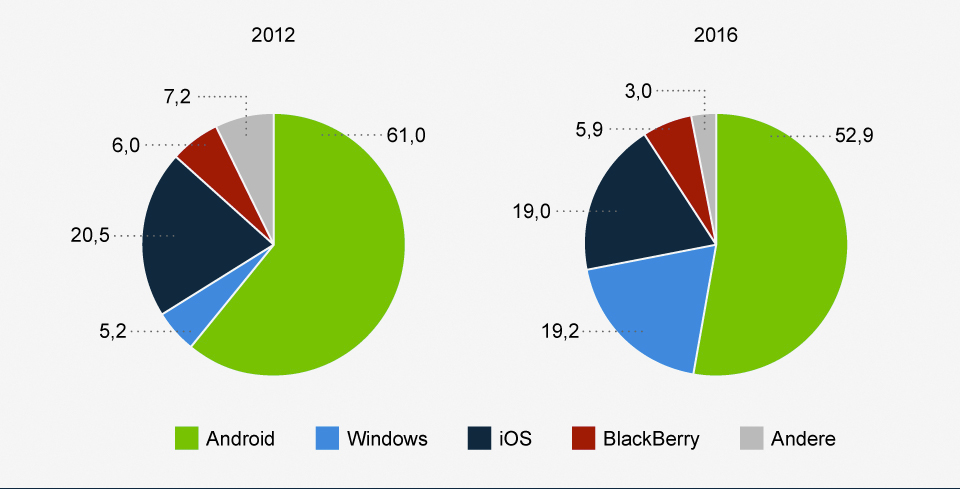
\includegraphics[scale=0.3]{bilder/smartphone_os_compare.png} \\
%			\multicolumn{1}{c}{
%				\ccLogo\ 
%				\begingroup
%    				\fontsize{8pt}{12pt}\selectfont
%    				\href{http://de.statista.com/}{Statista}; Lizenz: %\href{http://creativecommons.org/licenses/by-nd/4.0/}{CC BY-ND 4.0}
%				\endgroup
%			}
%		\end{tabulary}
%	\end{table}


%%%%%%%%%%%%%%%%%%%%%%%%%%%%%%%%%%%%%%%%%%%%%%%%%%%%%%%%%%%%%%
% System-Architektur
%%%%%%%%%%%%%%%%%%%%%%%%%%%%%%%%%%%%%%%%%%%%%%%%%%%%%%%%%%%%%%
\subsection{System-Architektur}\label{5_SA}
VoyageX ist als Webanwendung konzipiert, dementsprechend basiert die System- Architektur auf einem Client-Server-Modell. Die Darstellungsschicht wird in einem Browser am Client-Endgerät implementiert, während Persistenz- und die Kommunikationsschicht auf Client und Server verteilt werden. Anders als bei einer klassischen Client-Server-Implementierung mit rein Server-seitiger Datenhaltung ist bei kooperativen Systemen aus Gründen der Latenz-Optimierung oft eine replizierte Datenhaltung anzutreffen.\\ \\
Für eine im Offline-Modus nutzbare Anwendung ist eine Replikation aber sogar unumgänglich, demnach erhalten Clients lokale Kopien aller benötigten Anwendungsdaten. Geänderte und neu erstellte Daten werden zuerst lokal gespeichert, wodurch eine
%"`verteilte"'
Persistenz auch ohne Interaktion mit dem Server gewährleistet wird. Damit die Daten auch von anderen Benutzern bearbeitet werden können, werden sie aber so oft wie möglich mit der Master-Kopie am Server synchronisiert.\\
In den Abschnitten \ref{DBMS} und \ref{5_DSE} werden die Persistenz-Modelle von Server und Client ausführlicher beschrieben.\\ \\%, als Datenaustausch-Format wird JSON genutzt.
%Die Aufgaben einer serverseitigen Daten-API werden von einer Webanwendung übernommen welche in dieser Hinsicht eher mit der API eines WebServices verglichen werden kann.
%Eine weitere Aufgabe der Webanwendung ist die Benutzer-Authentisierung.\\ \\
Die Verteilung der Kommunikationsschicht wird in VoyageX mit der Publish-Subscribe-Messaging$^{\textbf{\ref{CMTPUBSUB}}}$%
\addtocounter{footnote}{1}%
\footnotetext{\label{CMTPUBSUB}Ein Muster zum Austausch von Nachrichten, bei dem letztere nicht direkt an den Empfänger, sondern in einen von (ggf. anonymen) Interessenten abonnierten "`Kanal"' geschrieben werden, aus dem diese die Nachrichten lesen können.}-Lösung von \texttt{Faye}$^{\textbf{\ref{CMTFAYE}}}$%
\addtocounter{footnote}{1}%
\footnotetext{\label{CMTFAYE}\href{http://faye.jcoglan.com/}{Faye - http://faye.jcoglan.com/}; letzter Zugriff: 22.04.2015}
implementiert, deren Server-Komponente, wie noch in Abschnitt \ref{RACK} beschrieben wird, als Modul in verschiedene Webserver integriert werden kann. Die Client- und Server-Komponenten von Faye werden sowohl im Frontend als auch im Backend hinter Schnittstellen gekapselt, so daß ein späterer Austausch der Kommunikations-Schicht- Implementierung möglich wird, ohne dafür weitere Anwendungs-Teile ändern zu müssen. Die einzelnen Module werden in \ref{5_MESSGNG} vorgestellt.\\ \\
In Abbildung \ref{fig:SYS_DEPLOY} ist die Verteilung einzelner Komponenten auf dem Client-Endgerät und dem Server zu sehen:
Die im nächsten Abschnitt beschriebene Single-Page-Anwendung bildet mit der Faye-Client-Komponente das \texttt{Frontend} im Web-Browser eines Benutzers, im \texttt{Backend} läuft eine Rack-Anwendung, die sowohl eine Rails - Web-Anwendung wie auch die Faye-Server-Komponente integriert. Im Produktions-Modus läuft Rack "`hinter"' einem Webserver.
  \begin{figure}[H]
      \centering
	  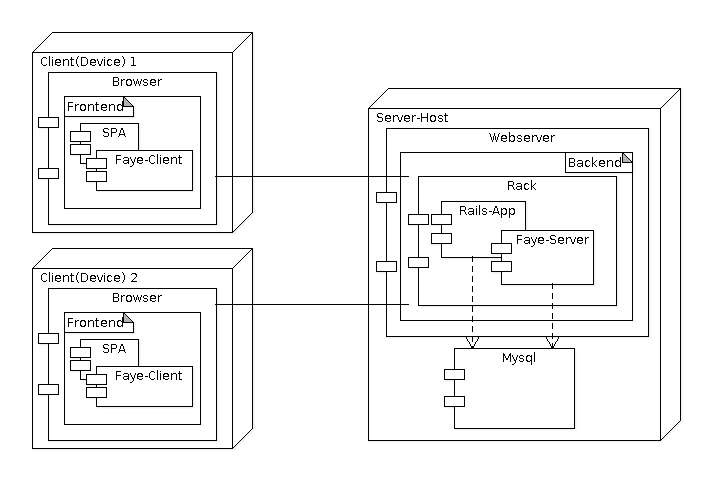
\includegraphics[scale=0.5]{bilder/system_architecture.png}
  	  \caption{Verteilung der System-Komponenten}
  	  \label{fig:SYS_DEPLOY}
  \end{figure}


%%%%%%%%%%%%%%%%%%%%%%%%%%%%%%%%%%%%%%%%%%%%%%%%%%%%%%%%%%%%%%
% Single Page Interface
%%%%%%%%%%%%%%%%%%%%%%%%%%%%%%%%%%%%%%%%%%%%%%%%%%%%%%%%%%%%%%
\subsection{Single Page Interface}\label{5_SPI}
% \noindent TODO: http://itsnat.sourceforge.net/php/spim/spi\_manifesto\_en.php
Bevor nun der Funktionsumfang von VoyageX vorgestellt wird, soll an dieser Stelle noch eine weiteres Implementierungs-Konzept vorgestellt werden, das die Aufgabenbereiche der System-Komponenten näher spezifiziert.\\
VoyageX ist als Single Page Interface-Application (SPI oder SPA) implementiert. Bei diesem Realisierungs-Konzept wird die gesamte Webanwendung über eine einzige Seite geladen, und alle möglichen Zustandswechsel innerhalb dieser Seite vollzogen. Damit werden folgende Ziele verfolgt:
\begin{itemize}[leftmargin=*,noitemsep,topsep=1ex,parsep=0pt,partopsep=0pt]
\item \textbf{User-Experience}: Die Implementierung als SPI ist vor allem für Webseiten mit ausgeprägtem Anwendungs-Charakter$^{\textbf{\ref{COMMENT_SPI_1}}}$ sinnvoll und bietet das für einen Benutzer vertraute Look-and-Feel einer Desktop-Anwendung.%
% footnotes
\addtocounter{footnote}{1}
\footnotetext{\label{COMMENT_SPI_1}Für Webseiten mit reinem Informations-Charakter, also für Eingabe und Darstellung rein textueller Daten, ist die über Urls definierte Status-Verwaltung des klassische Modells einfacher zu implementieren. Allerdings lassen sich mit der Integration von Rich-Client-Konzepten wie Ajax auch klassische Webseiten optimieren.}
\item \textbf{Performance}: Der Performancegewinn wird vor allem durch die Reduktion der Netzwerklast erreicht - Views werden bei einem SPI nicht am Server, sondern im Client aus Templates generiert, welche beim Anwendungsstart einmalig geladen werden. Der folgende Netzwerkverkehr wird also nicht mehr durch redundante View-Informationen aufgebläht, sondern beinhaltet nur noch die Daten-Synchronisation mit einem Backend. Die höhere Rechenlast am Client-Endgerät wird zusätzlich durch den von Rendering-Aufgaben entlasteten, schnelleren Server ausgeglichen.
\end{itemize}
\noindent
%Die Verlagerung der View-Logik zum Client wirft allerdings auch neue Probleme auf.\\
%So kann der Zustand der Anwendung nicht auf herkömmliche Art und Weise über ein Url-Lesezeichen referenziert werden, sondern muss anwendungsintern verwaltet werden
%Einzelne Anwendungs-Komponenten werden über Fragment-Identifier mit dem Anchor-Hash referenziert, wodurch eine SPI-Ansicht also mit beliebig komplexen Zuständen anstatt mit Seiten aufgebaut wird.
%\cite{SPI:MF}.\\
%Weitere Lösungen müssen für die Umsetzung von Search Engine Optimisations (SEO) gefunden werden. Dies ist für VoxageX im Rahmen dieser Arbeit zwar keine Anforderung - aber eine Suchmaschinen-Indizierung von PoI-Einträgen wäre sicher ein nützliches Feature.\\ \\
%Für die Realisierung der Anforderung nach Funktionsfähigkeit des Clients im Offline-Modus wird ein weiteres SPI-Konzept übernommen:
Die Abbildung \ref{fig:VIEW_GEN_SPI} zeigt, wie bei SPIs alle Ansichten (Views) der Anwendung mit Javascript-Logik aus Roh-Daten und Html-Templates über ein View-Model im Client erzeugt werden, wobei die Templates allesamt beim ersten Aufruf der Seite in den Browser geladen werden können. Auf diese Weise können neue PoI-Einträge in VoyageX auch im Offline-Modus erstellt und dargestellt werden.
Die Anwendungs-Daten können wahlweise über AJAX und / oder einen lokalen Speicher geladen und geschrieben werden. 
%Die weitere Kommunikation mit dem (Backend-)Server dient nur noch der Synchronisation der Daten und der Kommunikation mit anderen Clients.
% Diese Architektur ermöglicht es einem Benutzer jederzeit einen beliebigen Anwendungszustand auf einem verschiedenen Endgerät zu initialisieren.
%Allerdings beinhalten diese auch viele Lösungen, die für VoyageX nicht benötigt werden. Beispielsweise ist eine Data-Binding$^{\textbf{\ref{CMTDATABIN}}}$%
% footnote
%\addtocounter{footnote}{1}%
%\footnotetext{\label{CMTDATABIN}\href{http://en.wikipedia.org/wiki/Data\_binding}{Data Binding - http://en.wikipedia.org/wiki/Data\_binding}; letzter Zugriff: 01.03.2015} Lösung dafür gedacht, entfernte Objekte in die View zu integrieren. Bei VoyageX wird in der View aber nur mit lokalen Objekten gearbeitet die dann über eine Batch-Synchronisation mit den Systemdaten zusammengeführt werden.\\
	
%	\begin{table}[H]
%		\centering
%		\begin{tabulary}{\columnwidth}{C >{\centering}m{1cm} C}
%			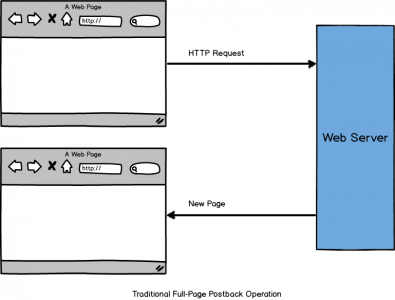
\includegraphics[scale=0.4]{bilder/spi_history_1.png} & & 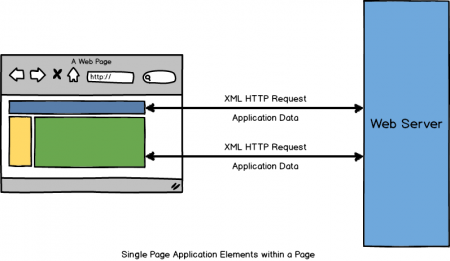
\includegraphics[scale=0.4]{bilder/spi_history_2.png} \\
%			\multicolumn{3}{c}{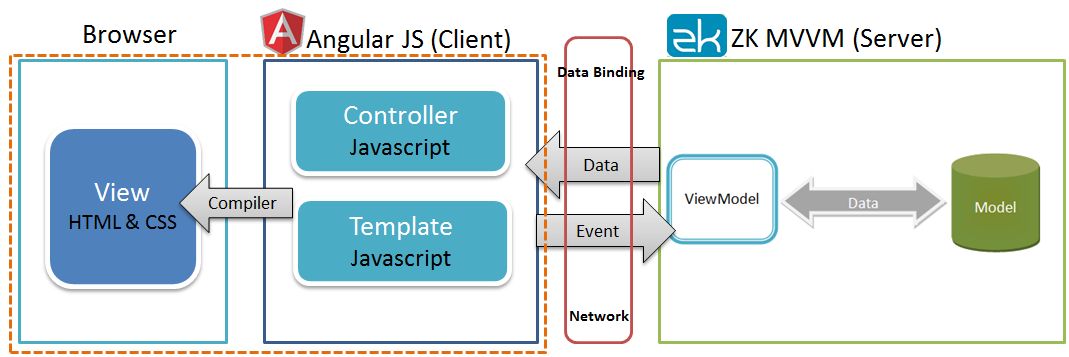
\includegraphics[scale=0.4]{bilder/zk-ng-architecture.png}}
%		\end{tabulary}
%	\end{table}
\enlargethispage{3\baselineskip} % allow 3 more lines on current page
  \begin{figure}[H]
  	\begin{adjustwidth}{-0.6cm}{0.6cm}
      \centering
	  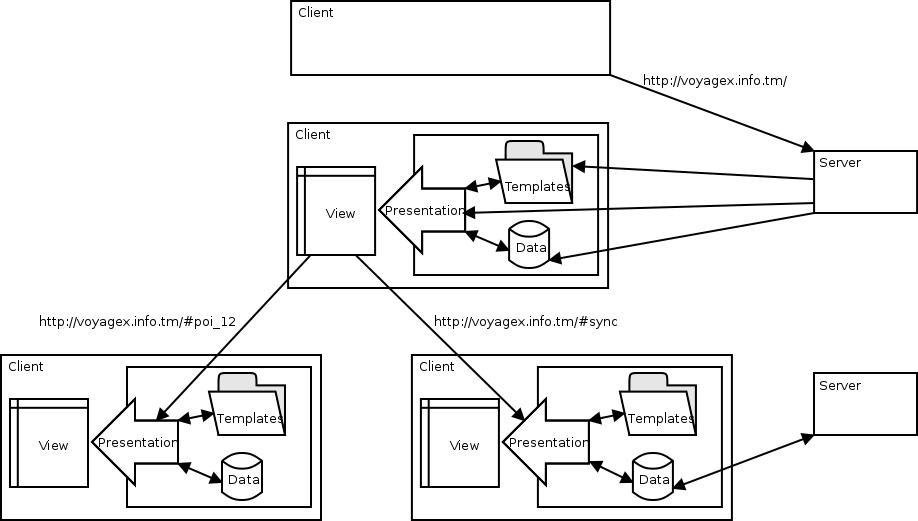
\includegraphics[scale=0.48]{bilder/spi.png}
  	  \caption{View-Generierung im SPI}
  	  \label{fig:VIEW_GEN_SPI}
  	 \end{adjustwidth}
  \end{figure}
\noindent
Es gibt verschiedene JS-Frameworks welche die Entwicklung einer SPI-Anwendung unterstützen (AngularJS$^{\textbf{\ref{WIKIANGULAR}}}$%
% footnote
\addtocounter{footnote}{1}%
\footnotetext{\label{WIKIANGULAR}\href{http://de.wikipedia.org/wiki/AngularJS}{AngularJS - http://de.wikipedia.org/wiki/AngularJS}; letzter Zugriff: 01.03.2015}
,  Ember.js$^{\textbf{\ref{WIKIEMBER}}}$%
% footnote
\addtocounter{footnote}{1}%
\footnotetext{\label{WIKIEMBER}\href{http://de.wikipedia.org/wiki/Ember.js}{Ember.js - http://de.wikipedia.org/wiki/Ember.js}; letzter Zugriff: 01.03.2015}
, Meteor$^{\textbf{\ref{WIKIMETEOR}}}$%
% footnote
\addtocounter{footnote}{1}%
\footnotetext{\label{WIKIMETEOR}\href{http://en.wikipedia.org/wiki/Meteor\_(web\_framework)}{Meteor - http://en.wikipedia.org/wiki/Meteor\_(web\_framework)}; letzter Zugriff: 01.03.2015}
). Für eine wenig komplexe Anwendung wie VoyageX würde die Nutzung eines derartigen Frameworks aber einen Overhead darstellen, außerdem wäre die durch die Wahl einer bestimmten Lösung bedingte Abhängigkeit für einen funktionalen Prototyp auch nicht sinnvoll.


\subsection{Funktionen}\label{4_FUNC}
%Es müssen in diesem Rahmen aber sowohl weitere Anwendungskomponenten (z.B. ein Benutzersystem) als auch Konzepte zur Benutzerführung (z.B. die Gestaltung von Arbeits-Menus) durch alle benötigten Funktionen entwickelt werden, um die fertige Anwendung testen zu können. Diese werden in Abschnitt \ref{4_BASEFUNC} beschrieben.

%%%%%%%%%%%%%%%%%%%%%%%%%%%%%%%%%%%%%%%%%%%%%%%%%%%%%%%%%%%%%%
% Basis-Funktionen für den testbaren Prototyp
%%%%%%%%%%%%%%%%%%%%%%%%%%%%%%%%%%%%%%%%%%%%%%%%%%%%%%%%%%%%%%
\subsubsection{Basis-Funktionen für den testbaren Prototyp}\label{4_BASEFUNC}
Damit die hier entwickelte Anwendung getestet werden kann, müssen neben den eigentlichen Funktionen auch noch weitere Anwendungskomponenten (z.B. ein Benutzersystem), sowie Konzepte zur Benutzerführung (z.B. die Gestaltung von Arbeits-Menus) durch alle benötigten Funktionen entwickelt werden.

\paragraph{Benutzerverwaltung}
%Die Bearbeitung von Karten und ein öffentlicher Nachrichten-Austausch
In einem kollaborativen Kontext müssen die Aktionen mehrer Benutzer synchronisiert werden, daher wird für VoyageX ein Benutzer und Autorisierungs-System benötigt.\\
Die Benutzer führen Aktionen aus, deren Ergebnisse im System gespeichert, und von anderen Benutzern wahrgenommen werden. Änderungen der System-Daten sollen dabei dem Autor zugeordnet werden können.\\ \\
Für die Realisierung des Benutzer-Systems sind folgende Komponenten erforderlich:
\begin{itemize}
  \item Registrierung
  \item Session-Verwaltung
\end{itemize}
%Eine über Einladung gesteuerte Gruppen-Verwaltung wäre sinnvoll und kann je nach Zeitverfügbarkeit optional implementiert werden.
%Es werden 2 Arten
%email passwort oder facebook
%andere benutzer können jeden sehen
%gruppenverwaltung wäre sinnvoll
%per einladung 

\paragraph{Darstellung der Karte und Bearbeitungs-Werkzeuge}
%Zur Darstellung einer Karte müssen aus den im vorigen Abschnitt vorgestellten API-Anbietern ein Tile-Service-Provider und ein Map-Viewer gewählt werden. Damit können folgende Grundfunktionen der Karten-Navigation implementiert werden:
In der graphischen Benutzeroberfläche wird eine Landkarte angezeigt. Diese ist interaktiv und es werden
folgende Navigations-Funktionen für die Berarbeitung von PoI-Einträgen implementiert:
\begin{itemize}
  \item Ein Benutzer kann durch "`ziehen"' der Karte, oder durch Eingabe von Koordinaten, jede beliebige Kartenposition im Browser-Fenster anzeigen lassen.
  \item Jeder Kartenausschnitt kann in mehreren Auflösungen (Zoom-Level) angezeigt werden.
  \item Es werden graphische Elemente in der Benutzeroberfläche bereitgestellt, mit denen Punkte auf der Karte optisch gekennzeichnet werden (Marker), sowie zusätzliche Informationen zu diesen Markierungen angezeigt werden können (Popups).
\end{itemize}
Zur Nutzbarmachung der Bearbeitungsfunktionen von VoyageX müssen Menus sowie Werkzeug- und Steuerungs-Elemente konzipiert und bereitgestellt werden, die dem Benutzer eine schnelle Interaktion und Navigation ermöglichen.

\paragraph{Erstellen von Einträgen}
Jeder registrierte Benutzer kann neue PoI-Einträge erstellen, indem er auf der Karte einen Punkt markiert und zu diesem über einen Eingabe-Dialog eine Beschreibung oder andere Informationen, wie beispielsweise eine angehängte Multimedia-Datei, speichert (Geo-Tagging). Diese Informationen sollen dann in einem Popup-Fenster über dem Marker des Eintrags angezeigt werden.\\
Alle anderen Benutzer können die Einträge (als Marker und Popups) sofort$^{\textbf{\ref{CMTFUNCERSEINT}}}$%
% footnote
\addtocounter{footnote}{1}%
\footnotetext{\label{CMTFUNCERSEINT}Oder sobald sie online sind.} ebenfalls auf ihren eigenen Endgeräten sehen, und weitere Texte und Anhänge hinzufügen.
%Ein Benutzer soll Informationen zu einem ausgewählten Standort speichern können. Neben einem obligatorischen Beschreibungs-Text soll auch eine Multimedia-Datei an die Beschreibung angehängt werden können\\ \\
%Benutzer sollen auch bereits existierende, selbst- oder durch andere Benutzer verfasste Einträge kommentieren können. Auch dabei soll der Anhang einer Multimedia-Anhang erlaubt sein.

%%%%%%%%%%%%%%%%%%%%%%%%%%%%%%%%%%%%%%%%%%%%%%%%%%%%%%%%%%%%%%
% Interaktion
%%%%%%%%%%%%%%%%%%%%%%%%%%%%%%%%%%%%%%%%%%%%%%%%%%%%%%%%%%%%%%
\subsubsection{Interaktion}
%VoyageX implementiert eine Infrastruktur für die Kommunikation zwischen Benutzern.
VoyageX bietet den Benutzern Funktionen für Kommunikation und Zusammenarbeit, wobei manche dieser Interaktionsfunktionen nur autorisiert ausgeführt werden können. Entfernte Benutzer müssen dazu erst mit deren Zustimmung als Kontakte gespeichert werden.
%Im Rahmen der Interaktion zwischen Benutzern sind auch durch Persönlichkeits-Rechte bedingte, besondere Sicherheits-Aspekte zu berücksichtigen. Dafür soll ein Benutzer die Möglichkeit haben, entsprechende Einstellungen vorzunehmen.

\paragraph{Follow-Rechteverwaltung}
Jeder Benutzer muß selbst festlegen, welche entfernten Benutzer (Peers) mit ihm in Interaktion
treten können.
%Die Erteilung einer entsprechenden Berechtigung kann nur über eine Anfrage an den gewünschten Interaktions-Partner, und mit seiner Zustimmung erfolgen.
Dazu gibt es in VoyageX die Möglichkeit, Autorisierungs-Anfragen an entfernte Benutzer zu stellen.
Wird die Interaktions-Berechtigung erteilt, gilt sie pauschal für alle Aktionen - eine gegliederte Rechteverwaltung kann optional für den Fall ausreichender zeiticher Resourcen implementiert werden.

\paragraph{Benachrichtigungen}
Alle online-Clients erhalten Echtzeit-Benachrichtigungen über neue PoI-Einträge oder -Kommentare, wobei diese Informationen dem Benutzer unterschiedlich präsentiert werden.
\begin{itemize}[leftmargin=*,noitemsep,topsep=1ex,parsep=0pt,partopsep=0pt]
\item Auf Änderungen durch Benutzer aus der Kontaktliste (Peers) wird mit optischen bzw. akkustischen Signalen hingewiesen
\item Auf Änderungen durch andere entfernte Benutzer wird nur hingewiesen, falls sich diese auf PoIs innerhalb eines begrenzten Umkreises um den aktuellen Standort des lokalen Benutzers beziehen.
\end{itemize}
%innerhalb eines vom Benutzer definierten Umkreises um den aktuellen Standort des Benutzers., außerdem werden diese auch sofort in der eigenen lokalen Ansicht jedes Benutzers angezeigt.
%\\ \\
Echtzeit-Benachrichtigungen erhält ein Benutzer auch über aktuelle Standorte von entfernten Benutzern aus der Kontaktliste. Voraussetzung hierfür ist die Aktivierung der Location-Sharing-Funktion, sowie, im Falle mobiler Endgeräte, auch von GPS, im Browser des Peers.%entfernten Benutzers.
%, kann er es entfernten Benutzern erlauben, Benachrichtigungen über seine eigenen Standort-Änderungen zu erhalten. Diese Funktion muss in der Anwendung explizit aktiviert bzw. deaktiviert werden.

\paragraph{Kommunikation}
Benutzer haben die Möglichkeit, über Instant Messaging miteinander zu kommunizieren. Dabei sind
folgende Chat-Typen implemetiert:
\begin{itemize}[leftmargin=*,noitemsep,topsep=1ex,parsep=0pt,partopsep=0pt]
\item \textbf{P2P-Chat}: Die ausgetauschten Nachrichten sind nur für 2 Kommunikationspartner sichtbar.
\item \textbf{Konferenz-Chat}: Mehrere Kommunikationspartner können sich am Chat beteiligen.
\end{itemize}
Die Nachrichten werden begrenzt gespeichert, d.h. daß ein Benutzer beim Wiederöffnen eines  geschlossenen Chat-Fensters oder nach dem Neustart der Anwendung einen limitierten Teil Nachrichten-Historie sehen kann.
Private Nachrichten werden nur von den beiden Kommunikationspartnern jeweils lokal gespeichert. Konferenz-Nachrichten werden zusätzlich im Backend gespeichert, und können so auch nach einem Wechsel auf ein anderes Endgerät angezeigt werden.

%\enlargethispage{3\baselineskip} % allow 3 more lines on current page
\paragraph{Kontakte lokalisieren}\label{LOCALIZE_CONTACTS}
Die bestätigten (entfernten) Kontakte werden auf der (lokalen) Karte jeweils mit einem Marker angezeigt.
%, über dessen Werkzeug-Menu die Interaktions-Funktionen gestartet werden können.
Zusätzlich zu dieser statischen Lokalisierung gibt es die Möglichkeit Bewegungs-Pfade eines entfernten Benutzers "`aufzuzeichnen"' (\texttt{Trace}), wofür aber GPS oder eine andere Positions-Bestimmungs-Funktion auf dem (mobilen) Endgerät des Peers aktiviert sein muß. Bei jeder empfangenen Positions-Änderung wird der Peer-Marker an die neue Position gesetzt, und eine Linie zur vorherigen Position gezeichnet.
 
\paragraph{Zeichnen auf entfernten Karten}\label{REMOTEDRAW}
%Jedem (entfernten) Peer ist auf der (lokalen) Karte eines Benutzers ein Marker zugeordnet. 
Eine weitere Interaktions-Form ergibt sich, wenn ein Peer die Position eines Markers auf einer entfernten Karte steuern kann. Anstatt der durch die Positions-Bestimmungs-Funktion des Endgeräts ermittelten Daten kann ein Benutzer auch manuell über Karten-Klicks definierte Positions-Daten senden, und damit den ihm zugeordneten entfernten Marker bewegen, wobei wie beim \texttt{Trace} die einzelnen Marker-Positionen mit Linien verbunden werden.
%Die Positions-Änderungen werden dann durch die Darstellung von Verbindungslinien in Form eines Pfades "`aufgezeichnet"'.
Auf diese Weise kann sich ein User von einem Peer beispielsweise navigatiorische Hilfestellung geben lassen.

%%%%%%%%%%%%%%%%%%%%%%%%%%%%%%%%%%%%%%%%%%%%%%%%%%%%%%%%%%%%%%
% Funktionsumfang im Offline-Betrieb
%%%%%%%%%%%%%%%%%%%%%%%%%%%%%%%%%%%%%%%%%%%%%%%%%%%%%%%%%%%%%%
\subsubsection{Funktionsumfang im Offline-Betrieb}
Folgende Anwendungsdaten müssen zum Erhalt der Funktionsfähigkeit im Offline-Betrieb vom Client eines Benutzers lokal gespeichert werden:
\begin{itemize}
  \item Karten-Kachel-Bilder
  \item PoI Einträge und Kommentare
  \item Konferenz- und P2P-Chat Nachrichten
  \item Peer-Daten
\end{itemize}
%Allerdings können nicht alle Kachel-Bilder der Weltkarte in allen Auflösungen lokal gespeichert werden. Das selbe gilt in Bezug auf die kompletten System-Daten. 
Aufgrund endlicher Speicher-Kapazität kann aber jeweils nur eine begrenzte Daten-Menge vorgehalten werden. Daher werden für jede Kategorie allgemeine und spezielle/eigene Cache-Strategien festgelegt, die automatisiert ausgeführt werden. Allgemein gilt:
	\begin{itemize}
		\item welche Bild-Dateien sollen vorab geladen und gespeichert werden? (Das schließt an dieser Stelle die Frage nach einer Verdrängungs-Strategie im Fall des Erreichens der Kapazitätsgrenze mit ein)% sollen
		%: Dafür muß ein Algorithmus gefunden und implementiert werden, der die vom Benutzer für die Bearbeitung benötigten Karten-Ausschnitte vorhersagt.
		\item wie sollen diese Bild-Dateien lokal gespeichert werden, bzw. welche Möglichkeiten bietet die Client-Plattform für die Speicherung?% sollen
	\end{itemize}
Alternativ oder aber auch in Kombination kann die Auswahl der zu speichernden Anwendungs-Daten manuell organisiert werden, wobei hierbei ebenso die Speicher-Limits berücksichtigt werden müssen.

%\enlargethispage{3\baselineskip} % allow 3 more lines on current page
\paragraph{Kartenkacheln}
Zur Anzeige von Karten werden einzelne Karten-Kacheln in verschiedenen Maßstäben von einem \texttt{Tile-Service} aus dem Internet geladen, und anschliessend zur Kartenansicht zusammengefügt (vgl. Abschnitt \ref{GL_TSP}). Die Cache-Strategie muß nun ein weiteres Problem berücksichtigen:
%Nachdem aber die Internet-Verbindung nicht immer garantiert ist muß eine Möglichkeit gefunden werden, die benötigten Bild-Dateien auch im Offline-Betrieb in die Kartenanzeige zu integrieren. Dabei sind Lösungen zu finden, 
%Für eine Netzwerk-Verbindungs-unabhängige Karten-Darstellung werden folgende Probleme von VoyageX entschieden: 
	\begin{itemize}
		\item wie können diese Bild-Dateien dann vom \texttt{Map-Viewer} eingebunden werden% können
	\end{itemize}
%kann indirekt über die im nachfolgenden Abschnitt beschriebene Bookmark-Funktion durchgeführt werden.

\paragraph{PoI-Einträge}
Im Backend$^{\textbf{\ref{CMTBEREF1}}}$%
% footnote
\addtocounter{footnote}{1}%
\footnotetext{\label{CMTBEREF1}Das Backend wird in Abschnitt \ref{5_BE} ausführlich beschreiben.} werden alle PoI-Einträge des Systems gespeichert - jeder Client speichert lokal eine Kopie der für ihn relevanten System-Daten (vgl. Abschnitt \ref{5_SA}), das sind:
	\begin{itemize}
		\item PoIs in einem definierten Umkreis um den aktuellen Standort des Benutzers
		\item vom Benutzer explizit mit einem Lesezeichen markierte PoIs
	\end{itemize}
%lokal können aber je nach Speicher-Kapazität nur eine begrenzte Anzahl von Einträgen gespeichert werden.\\
%Die Cache-Kriterien für PoIs stellen aber auch Kriterien für die Speicherung von Kartenkachel-Bildern dar.
%PoI-Einträge beziehen sich immer auf bestimmte Karten-Positionen, also wirkt sich die Entscheidung über die Auswahl der lokal zu speichernden Einträge auch auf die Wahl der Karten-Kacheln aus.
Soll ein Poi im offline-Modus angezeigt werden, dann ist auch eine Anzeige des zugehörigen Kartenbereichs sinnvoll, also müssen neben den PoI-Daten auch die Karten-Kachel-Bilder vorgehalten werden.
%Allerdings wird bei Einträgen ein zusätzliches Relevanz-Kriterium eingeführt: vom Benutzer explizit markierte Einträge (Bookmarks) sind jederzeit verfügbar, d.h. daß nicht nur die Bookmark-Information sondern auch der referenzierte Kartenbereich lokal persistent gehalten wird.\\
%werden immer dann mit den system-daten synschronisiert wenn der benutzer online ist.\\
%Bookmarks werden nur lokal gespeichert.

\paragraph{Nachrichten}
Anders als bei PoI-Einträgen existiert für Chat-Nachrichten in VoyageX kein Karten-Kontext, und folglich besteht auch keine Notwendigkeit Karten-Kachel-Bilder dafür zu laden. Aus diesem Grund kann die Speicher-Begrenzung für
Chat-Nachrichten mit einem einfachen Cache-Algorithmus, wie beispielsweise einer einer FIFO-History-Queue, implementiert werden. Für eine ortsbezogene Kommunikation wird in VoyageX das Einfügen von PoI-Links in eine Chat-Nachricht angeboten.

\paragraph{Peer-Daten}
Peer-Daten werden sowohl von PoI-Einträgen wie auch von Chat-Nachrichten referenziert. Für den Offline-Betrieb werden zunächst alle Peer-Daten lokal gespeichert, im Falle einer Kapazitäts-Überschreitung muss aber ein Cache-Algorithmus angewandt werden. Möglich wäre auch hier ein Bezug zum Standort des lokalen Benutzers oder eine Least Recently Used (LRU)$^{\textbf{\ref{CMTLRU}}}$%
% footnote
\addtocounter{footnote}{1}%
\footnotetext{\label{CMTLRU}\href{http://en.wikipedia.org/wiki/Cache\_algorithms\#Examples}{LRU - http://en.wikipedia.org/wiki/Cache\_algorithms\#Examples}; letzter Zugriff: 08.05.2015} Strategie.
%Sie werden sowohl im Backend wie auch lokal gespeichert, allerdings werden aber getrennt.
%, deshalb werden sie für deren vollständige Anzeige benötigt. 
%Peer-Daten werden sowohl im Backend als auch lokal gespeichert.

\subsubsection{Synchronisation}
Wenn ein Benutzer für einen bestimmten Zeitraum offline war, kann eine Synchronisation
der lokalen Daten mit den System-Daten in folgenden Fällen erforderlich werden:
	\begin{itemize}
		\item der Benutzer hat selbst zwischenzeitlich neue Einträge erstellt, geändert oder gelöscht
		\item andere Benutzer haben zwischenzeitlich neue Einträge erstellt, geändert oder gelöscht
	\end{itemize}
Sobald der Benutzer nach einer Netzwerk-Verbindungs-Unterbrechung wieder online ist, muß sein Client mit dem Backend einen Daten-Abgleich durchführen. Falls der Benutzer Daten geändert hat muß das Backend alle anderen online-Clients über die Änderungen informieren, damit die Clients wiederum ihr eigenes lokales Cache synchronisieren können.
%Im Rahmen dieser Arbeit soll ein Prototyp einer Web-Awendung für kooperatives Geo-Tagging entwickelt werden. In Abschnitt \ref{2_VOYAGEX} folgt eine Beschreibung der gewünschten Funktionen. 
%Es müssen in diesem Rahmen aber sowohl weitere Anwendungskomponenten (z.B. ein Benutzersystem) als auch Konzepte zur Benutzerführung (z.B. die Gestaltung von Arbeits-Menus) durch alle benötigten Funktionen entwickelt werden, um die fertige Anwendung testen zu können. Diese werden in Abschnitt \ref{4_BASEFUNC} beschrieben.

\newpage
%%%%%%%%%%%%%%%%%%%%%%%%%%%%%%%%%%%%%%%%%%%%%%%%%%%%%%%%%%%%%%
% Anwendungsfälle für VoyageX
%%%%%%%%%%%%%%%%%%%%%%%%%%%%%%%%%%%%%%%%%%%%%%%%%%%%%%%%%%%%%%
%\enlargethispage{3\baselineskip} % allow 3 more lines on current page
\subsection{Anwendungsfälle}\label{4_UC}
%In Abschnitt \ref{2_VOYAGEX} wurden Funktionen beschrieben, die für die Anwendung entwickelt werden sollen.
%Wie bereits erwähnt werden aber noch weitere Funktionen benötigt um einen testbaren Anwendungs-Prototypen zu erstellen.
Mit den im vorigen Abschnitt beschriebenen Funktionen lassen sich nunmehr die Anwendungsfälle für VoyageX bilden.

%\subsubsection{Actors}
%%\begin{enumerate}[labelwidth=0pt,leftmargin=39pt,noitemsep,topsep=0pt,parsep=0pt,partopsep=0pt]
%\begin{itemize}[leftmargin=*,noitemsep,topsep=1ex,parsep=0pt,partopsep=0pt]
%\item \textbf{Benutzer}: Der lokale Benutzer in einem initiierenden Zustand
%\item \textbf{Wahrnehmer}: Der lokale Benutzer in einem induzierten Zustand
%\item \textbf{Peer}: Ein anderer / entfernter Benutzer
%\item \textbf{Comm}: Die Kommunikations-Schicht
%\item \textbf{Backend}: Die Synchronisations-Schicht
%\end{itemize}

\subsubsection{Rolle \textbf{Benutzer}}
Dieser Actor ist der lokale Benutzer, der auf seinem Endgerät mit der Anwendung aktiv arbeitet, also die Bedienungs- und Werkzeug-Elemente der Anwendung benutzt.\\
	%\begin{table}[label=usecases-benutzer,h!]
	\begin{table}[H]\label{usecases-benutzer}
		\centering
		\begin{tabulary}{\linewidth}{|>{\centering}m{1cm}|L|C|C|C|C|C|}
		\hline
			\textbf{Ref} & \textbf{Name} & \textbf{online} & \textbf{offline} & \textbf{synchron} & \textbf{asynchron} & \textbf{visibility} \\ \hline
			\ref{subsubsec:uc_reg} & Registrieren & y & n & y & n & - \\ \hline
			\ref{subsubsec:uc_anm} & Anmelden & y & n & y & n & \# \\ \hline
			\ref{subsubsec:uc_locmapnav} & Lokale Karte navigieren & y & y & y & n & \# \\ \hline
			\ref{subsubsec:uc_remmapnav} & Zeichnen auf entfernten Karten & y & n & y & n & \# \\ \hline
			\ref{subsubsec:uc_poinew} & PoI markieren & y & y & y & y & + \\ \hline
			\ref{subsubsec:uc_poinote} & PoI kommentieren & y & y & y & y & + \\ \hline
			\ref{subsubsec:uc_poibookmark} & Poi merken (Bookmark/Notiz) & y & y & n & n & - \\ \hline
			\ref{subsubsec:uc_locnote} & Ort merken (Bookmark/Notiz) & y & y & n & n & - \\ \hline
			\ref{subsubsec:uc_reqmefollowpeer} & "`Folgen"' beantragen & y & y & y & y & \# \\ \hline
			\ref{subsubsec:uc_grantpeerfollowme} & "`Folgen"' erlauben & y & y & y & y & \# \\ \hline
			\ref{subsubsec:uc_denypeerfollowme} & "`Folgen"' verweigern & y & y & y & y & \# \\ \hline
% wird vom nächsten usecase-block erfasst
%			Aktionen anderer Benutzer wahrnehmen & y & n & y & y & \# \\ \hline
			\ref{subsubsec:uc_usernote} & Notiz zu anderem Benutzer erstellen & y & y & n & n & - \\ \hline
			\ref{subsubsec:uc_chatp2p} & P2P-Chat & y & y & y & y & \# \\ \hline
			\ref{subsubsec:uc_chatconf} & Konferenz & y & y & y & y & \# \\ \hline
		\end{tabulary}
	\caption{Benutzer-Use-Cases}
	\end{table}
\begin{itemize}[leftmargin=*,noitemsep,topsep=1ex,parsep=0pt,partopsep=0pt]
\item \textbf{online}: der Anwendungsfall tritt im Online-Modus auf.
\item \textbf{online}: der Anwendungsfall tritt im Offline-Modus auf.
\item \textbf{synchron}: Die Daten und Aktionen auf dem lokalen System können in Echtzeit mit dem Backend und somit mit allen Online-Benutzern synchronisiert werden, vorausgesetzt das lokale System ist online. 
\item \textbf{asynchron}: Die Daten und Aktionen auf dem lokalen System können asynchron mit dem Backend abgeglichen werden, der Anwendungsfall erfordert keine synchrone Kooperation.
\item \textbf{visibility}: Bezeichnet die Sichtbarkeit von Daten und Wahrnehmung von Aktionen - oder deren kooperativen Character - für andere Benutzer.
%\renewcommand{\labelitemii}{*}
	\begin{itemize}[leftmargin=*,noitemsep,topsep=1ex,parsep=0pt,partopsep=0pt]
	%\begin{itemize}[label={},labelwidth=0pt,leftmargin=24pt,noitemsep,topsep=0pt,parsep=0pt,partopsep=0pt]
\renewcommand{\labelitemii}{\textbf{+}}
		\item \textbf{public}: Die Daten und Aktionen sind für alle Benutzer sichtbar
\renewcommand{\labelitemii}{\textbf{\#}}
		\item \textbf{protected}: Die Daten und Aktionen sind für ausgewählte Benutzer und/oder nur unter bestimmten Bedingungen sichtbar
\renewcommand{\labelitemii}{\textbf{-}}
		\item \textbf{private}: Daten und Aktionen können von anderen Benutzern nicht wahrgenommen werden.
	\end{itemize}
\end{itemize}


\paragraph{Die Rollen \textbf{Wahrnehmer} und \textbf{Peer}}
Wahrnehmer ist die passive Rolle eines Benutzers, in der er über Änderungen des Verbindungs-Zustands, Änderungen der System-Daten oder Aktivitäten anderer Benutzer benachrichtigt wird.\\
\texttt{Peer} bezeichnet den Benutzer in seiner Rolle als entfernter Benutzer und Kontakt eines lokalen Benutzers.\\
	\begin{table}[H]
		\centering
		\begin{tabulary}{\columnwidth}{|>{\centering}m{1cm}|L|C|C|C|C|C|}
		\hline
			\textbf{Ref} & \textbf{Name} & \textbf{online} & \textbf{offline} & \textbf{synchron} & \textbf{asynchron} & \textbf{visibility} \\ \hline
			\ref{subsubsec:uc_watchconnstate} & Änderung des Internetverbindungs-Status & y & y & y & n & - \\ \hline
			\ref{subsubsec:uc_watchgrantmefollowpeer} & Berechtigung zur Wahrnehmung von Aktionen eines anderen Benutzers erhalten & y & n & y & y & \# \\ \hline
			\ref{subsubsec:uc_watchposofpeer} & Position/Bewegung anderer Benutzer im Nahbereich & y & n & y & y & \# \\ \hline
			\ref{subsubsec:uc_watchpoinewornotebypeer} & Neue PoI-Einträge oder -Kommentare & y & n & y & y & \# \\ \hline
			\ref{subsubsec:uc_watchmsgbypeer} & Neue P2P- oder Konferenz-Nachrichten & y & n & y & y & \# \\ \hline
		\end{tabulary}
	\end{table}

\subsubsection{Rolle \textbf{Comm}}
In der Kommunikations-Schicht sind Interaktions-Funktionen implementiert. Nachrichten werden über die Publish / Subscribe Infrastruktur verteilt.\\
	\begin{table}[H]
		\centering
		\begin{tabulary}{\columnwidth}{|L|C|C|C|C|C|}
		\hline
			\textbf{Name} & \textbf{online} & \textbf{offline} & \textbf{synchron} & \textbf{asynchron} & \textbf{visibility} \\ \hline
			Benachrichtigungen über Bewegungsdaten/Standort von Benutzern & y & n & y & n & \# \\ \hline
			Benachrichtigungen über neue PoI-Einträge & y & n & y & n & \# \\ \hline
			P2P- und Konferenz-Chat-Meldungen & y & n & y & n & \# \\ \hline
		\end{tabulary}
	\end{table}

\subsubsection{Rolle \textbf{Backend}}
Das Backend übernimmt Benutzer-Verwaltungs und Synchronisations-Aufgaben. Für das Versenden von System-Nachrichten werden die Funktionen der Kommunikations-Schicht genutzt.\\
	\begin{table}[H]
		\centering
		\begin{tabulary}{\columnwidth}{|L|C|C|C|C|C|}
		\hline
			\textbf{Name} & \textbf{online} & \textbf{offline} & \textbf{synchron} & \textbf{asynchron} & \textbf{visibility} \\ \hline
			Synchrone Integration von Daten-Änderungen durch Online-Benutzer & y & n & y & - & \# \\ \hline
			Asynchrone Integration von Daten-Änderungen durch wiederverbundene Offline-Benutzer & y & n & - & y & \# \\ \hline
			Benachrichtigung an Benutzer über eine Anfrage zur Wahrnehmung durch einen anderen Benutzer & y & n & y & y & \#  \\ \hline
			Benachrichtigung an Benutzer über Erlaubnis zur Wahrnehmung eines anderen Benutzers & y & n & y & y & \#  \\ \hline
		\end{tabulary}
	\end{table}
\vspace{2ex}
\noindent
Nachdem die funktionalen Anforderungen nunmehr festgelegt und die Aufgabenbereiche verteilt sind, wird in den folgenden Abschnitten näher auf die technischen Implementierungs-Details der Anwendungskomponenten \texttt{Backend} und \texttt{Frontend} eingegangen.

%%%%%%%%%%%%%%%%%%%%%%%%%%%%%%%%%%%%%%%%%%%%%%%%%%%%%%%%%%%%%%
% Backend
%%%%%%%%%%%%%%%%%%%%%%%%%%%%%%%%%%%%%%%%%%%%%%%%%%%%%%%%%%%%%%
\subsection{Backend}\label{5_BE}
Der Backend-Server erfüllt folgende Aufgaben:
	\begin{itemize}
		\item Bereitstellung der Installations-Konfiguration für die Anwendungs-Initialisierung (SPI)
		\item Benutzerverwaltung des Systems
		\item Synchronisation der System-Daten für alle Benutzer
		\item Bereitstellung der Kommunikations-Infrastruktur
	\end{itemize}

\subsubsection{Ruby-On-Rails}
Die Backend-Dienste werden als Ruby-On-Rails$^{\textbf{\ref{COMMENT_ROR_1}}}$ (RoR) Web-Anwendung implementiert.%
% footnotes
\addtocounter{footnote}{1}
\footnotetext{\label{COMMENT_ROR_1}Ruby-On-Rails ist ein in der Programmiersprache Ruby geschriebenes Open-Source-Web-Framework mit dem unter anderem durch das "Convention over Configuration" Prinzip eine hohe Produktivität durch schnelle Anwendungs-Entwicklung (Rapid-Application-Development - RAR) erreicht werden kann. \cite{ROR:GETSTA}}%
Seit RoR-Version 2.3 wird \texttt{Rack} als Standard-Web-Schnittstelle für RoR-Anwendungen genutzt. \cite{WIKI:RACK_SINCE_2.3}. Da neben der RoR-Webapp noch eine weitere Rack-Anwendung in VoyageX integriert ist, wird Rack im nächsten Abschnitt etwas genauer betrachtet.\\
Wie für alle verbreiteten Programmiersprachen gibt es für Ruby auch zahlreiche Hilfs-Bibiotheken, in der Ruby-Welt \texttt{Gems} genannt, deren modularisierte Funktionalität mit geringem Aufwand in eine RoR-App integriert werden kann $^{\textbf{\ref{GEMINFO1}}}$.%
% footnotes
\addtocounter{footnote}{1}%
\footnotetext{\label{GEMINFO1}Viele Gems sind Open-Source-lizensiert}
Konkret ist damit die Integration Anwendungs-spezifischer Gems gemeint, denn Rails selbst setzt sich bereits aus verschiedenen Gems zusammen, eines davon ist eben auch Rack.\\
Im folgenden werden nach Rack auch noch einige VoyageX-spezifischen Gems vorgestellt.

\paragraph{Rack}\label{RACK}
Rack definiert eine minimale API um Webserver mit Web-Frameworks zu verbinden \cite{RACK:INTRO}.
Diese API besteht aus einer einzigen Methode \texttt{call}, welche mit dem Aufruf-Parameter \texttt{env} ein Http-Request-Objekt sowie Laufzeit-Umgebungs-Informationen an eine Rack-Anwendung übergibt, und als Rückgabe eine Http-Response erwartet, welche dann an den Client zurückgesendet wird.\\
Die Integration anwendungsspezifischer Netzwerk-Funktionalität wird durch konfigurierbare \texttt{Middleware}-Komponenten ermöglicht. So wird beispielsweise in VoyageX die Kommunikations-Schicht durch die Faye-Middleware-Komponente implementiert, welche den Webserver um eigene, für die RoR-Anwendung völlig transparente, Protokolle erweitert (siehe Abschnitt \ref{Faye}).\\ \\
% Rails-Anwendungen sind Rack-Anwendungen
In der Praxis werden Rack-Apps (also auch RoR-Anwendungen) in einer Produktions-Umgebung als Plugins von "`kompletten"' Webservern wie nginx$^{\textbf{\ref{NGINXIDX}}}$%
\addtocounter{footnote}{1}%
\footnotetext{\label{NGINXIDX}\href{http://nginx.org/}{http://nginx.org/}; letzter Zugriff: 22.01.2015}
oder Apache$^{\textbf{\ref{APACHEIDX}}}$%
\addtocounter{footnote}{1}%
\footnotetext{\label{APACHEIDX}\href{http://httpd.apache.org/}{http://httpd.apache.org/}; letzter Zugriff: 22.01.2015}
eingebunden, da bei diesen weitere und optimierte Webserver-Funktionen genutzt werden können, deren genauere Untersuchung jedoch keine weiteren Erkenntnisse zu VoyageX liefern würde, und darum an dieser Stelle der Hinweis darauf genügen soll.

\paragraph{VoyageX-spezifische Gems}\noindent
Die in einer RoR-App eingebundenen Hilfsbibliotheken können nach verschiedenen Kritierien kategorisiert werden.
	\begin{itemize}
		\item Laufzeit-Umgebung
		\item Infrastruktur
		\item Anwendungslogik
	\end{itemize}
In Ruby-Anwendungen, also auch in Rails-Webanwendungen, werden häufig Module oder Bibliotheken mittels RubyGems eingebunden, um bereits verfügbare Lösungen nicht selbst programmieren zu müssen$^{\textbf{\ref{CMT_GEM}}}$%
\addtocounter{footnote}{1}%
\footnotetext{\label{CMT_GEM}Nicht alle Gems werden als OpenSource angeboten}
. Viele allgemeine Gems einer Rails-App werden quasi standardmäßig genutzt, dazu zählen Syntactic-Sugar Gems wie Haml$^{\textbf{\ref{HAMLIDX}}}$%
\addtocounter{footnote}{1}%
\footnotetext{\label{HAMLIDX}\href{http://haml.info/}{haml - http://haml.info/}; letzter Zugriff: 22.01.2015}
und Sass$^{\textbf{\ref{SASSIDX}}}$%
\addtocounter{footnote}{1}%
\footnotetext{\label{SASSIDX}\href{http://sass-lang.com/}{sass - http://sass-lang.com/}; letzter Zugriff: 22.01.2015}
, oder aber Code-Bibliotheken wie jQuery$^{\textbf{\ref{JQUERYIDX}}}$%
\addtocounter{footnote}{1}%
\footnotetext{\label{JQUERYIDX}\href{https://jquery.com/}{jQuery - https://jquery.com/}; letzter Zugriff: 22.01.2015}.\\ \\
VoyageX-spezifische Gems sind:\\
\lstset{language=CoffeeScript}
\begin{lstlisting}[frame=single,xleftmargin=0pt,numbers=none]
  gem "devise"
  gem "omniauth-facebook"
  gem "geocoder"
  gem "paperclip", "~> 4.2"
  group :production, :staging, :development do
    gem "comm", path: "comm-plugin"
  end
  gem "resque-scheduler" 
\end{lstlisting}

\subparagraph{devise$^{\textbf{\ref{INFO_DEVISE}}}$:}%
\addtocounter{footnote}{1}%
\footnotetext{\label{INFO_DEVISE}\href{https://github.com/plataformatec/devise/blob/master/README.md}{Devise - https://github.com/plataformatec/devise/blob/master/README.md}; letzter Zugriff: 04.05.2015}
Ein Autorisierungs-Paket, das konfigurierbare Implementierungen von Registrierungs-Logik mit optional erforderlicher Email-Bestätigung, über Session-Verwaltung, bis hin zur Authentisierung durch Dritte, also beispielsweise Social Networks wie Facebook und Twitter, oder aber auch LDAP enthält.\\
Verschiedene Strategien werden als Plugins in Devise integriert. In der Anwendung sind dann Utility-Methoden
verfügbar, wie beispielsweise:
\lstset{language=Ruby}
\begin{lstlisting}[frame=single,xleftmargin=0pt,numbers=none]
  current_user
  signed_in?
\end{lstlisting}
\subparagraph{omniauth-facebook$^{\textbf{\ref{INFO_OMNIFB}}}$:}%
\addtocounter{footnote}{1}%
\footnotetext{\label{INFO_OMNIFB}\href{https://github.com/mkdynamic/omniauth-facebook/blob/master/README.md}{Omniauth-Facebook - https://github.com/mkdynamic/omniauth-facebook/blob/master/README.md}; letzter Zugriff: 04.05.2015}Die Implementierung einer Devise-Strategie für die Authentisierung über ein Facebook-Account. Im View-Code muss nur noch, wie im folgenden Haml-Snippet, ein Link eingebettet werden, den Rest erledigt das Gem:
\begin{lstlisting}[frame=single,xleftmargin=0pt,numbers=none]
.button.facebook_login
  = link_to image_tag("fb-icon.png"), user_omniauth_authorize_path(:facebook)
\end{lstlisting}

\subparagraph{paperclip$^{\textbf{\ref{INFO_PAPERCL}}}$:}%
\addtocounter{footnote}{1}%
\footnotetext{\label{INFO_PAPERCL}\href{https://github.com/thoughtbot/paperclip/blob/master/README.md}{Paperclip - https://github.com/thoughtbot/paperclip/blob/master/README.md}; letzter Zugriff: 04.05.2015}
Paperclip bietet Funktionen zur Bearbeitung und Verwaltung hochgeladener Dateien in Active-Record. Die Dateien können auch über Konfigurations-Parameter automatisiert vor- und nach-bearbeitet werden, beispielsweise können Bilder skaliert und/oder in verschiedene Formate konvertiert werden.
\begin{lstlisting}[frame=single,xleftmargin=0pt,numbers=none]
  current_user.avatar(:medium_size)
\end{lstlisting}
\subparagraph{resque$^{\textbf{\ref{INFO_RESQUE}}}$:}%
\addtocounter{footnote}{1}%
\footnotetext{\label{INFO_RESQUE}\href{https://github.com/resque/resque/blob/master/README.md}{Resque - https://github.com/resque/resque/blob/master/README.md}; letzter Zugriff: 04.05.2015}
ist eine Redis-Db$^{\textbf{\ref{RAILSENG}}}$%
\addtocounter{footnote}{1}%
\footnotetext{\label{RAILSENG}\href{http://de.wikipedia.org/wiki/Redis}{Redis - http://de.wikipedia.org/wiki/Redis}; letzter Zugriff: 22.01.2015}%
-gestützte Bibliothek zur Ausführung asynchroner Jobs. Komplexe bzw. aufwendige Operationen sollten nicht im Request-Response Zyklus der Webanwendung ausgeführt werden da sonst
der Server blockieren könnte. In VoyageX wird Resque bei der Synchronisation der Benutzer-Daten-Kopie mit der Master-Kopie eingesetzt. Das Kommunikations-Modul von Faye nutzt Resque ebenfalls.
\subparagraph{comm:}comm ist ein für VoyageX entwickeltes Ruby-Gem, das die Kommunikations - Infrastruktur kapselt, indem deren Anwendungsfunktionen in einem eigenen Rails - Engine$^{\textbf{\ref{RAILSENG}}}$%
\addtocounter{footnote}{1}%
\footnotetext{\label{RAILSENG}\href{http://api.rubyonrails.org/classes/Rails/Engine.html}{Rails-Engine http://api.rubyonrails.org/classes/Rails/Engine.html}; letzter Zugriff: 22.01.2015}
(mit eigenem Rack - Middleware - Stack) ausgeführt werden$^{\textbf{\ref{RAILSENG}}}$%
\addtocounter{footnote}{1}%
\footnotetext{\label{RAILSENG}Zur Laufzeit hat das Plugin aber Zugriff auf alle Resourcen der Anwendung}.
Diese Kapselung ermöglicht eine freie Auswahl aus Kommunikations-Lösungen verschiedener Anbieter.\\
%Durch diese Trennung kann VoyageX jederzeit auf ein anderes Kommunikations-System umgestellt, und der Faye-spezifische Teil ersetzt werden.\\
Neben der bereits gezeigten Deklaration im Gem-File muss das Plugin noch mittels Eintrag in der Konfigurations-Datei \texttt{config/routes.conf} in die Anwendung integriert werden, damit alle Requests, die mit einem festzulegenden Url-Pfad-Prefix (hier \texttt{/comm}) beginnen, zur Abarbeitung an das Plugin weitergereicht werden:
\begin{lstlisting}[frame=single,xleftmargin=0pt,numbers=none]
  mount FayeComm::Engine => "/comm"
\end{lstlisting}
In der Datei \texttt{comm-plugin/lib/faye\_comm/engine.rb} wird die Plugin-eigene Middleware konfiguriert: 
\lstset{language=CoffeeScript}
\begin{lstlisting}[frame=single,xleftmargin=0pt,numbers=none]
module FayeComm
  class Engine < ::Rails::Engine
  	engine_params = {...}
    config.middleware.use FayeRails::Middleware, { mount: '/', timeout: 25 }.merge!(engine_params) do
      map '/**' => FayeComm::ChannelsController
    end
  end
end
\end{lstlisting}
Die dafür erforderlichen Gems werden in \texttt{comm-plugin/comm.gemspec} eingetragen.
\lstset{language=CoffeeScript}
\begin{lstlisting}[frame=single,xleftmargin=0pt,numbers=none]
  s.add_dependency "faye-rails", "2.0.0"
\end{lstlisting}

\subparagraph{faye-rails$^{\textbf{\ref{INFO_FAYRAI}}}$:}\label{FAYERAILS}%
\addtocounter{footnote}{1}%
\footnotetext{\label{INFO_FAYRAI}\href{https://github.com/jamesotron/faye-rails/blob/master/README.md}{Faye-Rails - https://github.com/jamesotron/faye-rails/blob/master/README.md}; letzter Zugriff: 04.05.2015}
Faye-Rails ist die vom FayeComm-Plugin eingebundene Rack-Middleware, welche
die Server-Komponente des Public-Messaging-Systems \texttt{Faye} implementiert. Faye bietet ihrerseits widerum eine Schnittstelle zur Integration Anwendungs-spezifischer Funktionen in die Kommunikations-Abläufe. Dafür wird in VoyageX der in \ref{CTRLS_CHANNEL} beschriebene Controller eingesetzt.
 
\paragraph{Controllers}\noindent
Rails unterstützt URL - Mapping nach dem \texttt{Representational State Transfer (Rest)}$^{\textbf{\ref{CMTREST}}}$%
\addtocounter{footnote}{1}%
\footnotetext{\label{CMTREST}\href{http://de.wikipedia.org/wiki/Representational\_State\_Transfer}{ReST - http://de.wikipedia.org/wiki/Representational\_State\_Transfer}; letzter Zugriff: 22.01.2015} Paradigma. Dieses zielt auf einen über URL-Format und Request-Methode standardisierten Resourcen-Zugriff ab, um ähnlich wie bei Web-Services auch ohne Kenntnis der Implementierung eines Dienstes bestimmte Standard-Operationen wie z.b. Create, Read, Update und Delete (CRUD) auf Resourcen durchführen zu können. Zusätzlich werden durch weitere Request-Parameter (Accept-Header) auch die Daten-Repräsentations/Ausgabe-Formate der Resource beim Aufruf festgelegt.\\
Jede Url wird in Rails auf einen Methode (Action) eines Controllers verlinkt (gemapped). Diese Zuordnung
wird in der datei \texttt{config/routes.rb} konfiguriert.\\
Folgender Eintrag erzeugt beispielsweise ein Mapping für 
\texttt{PUT} -Requests auf die URL \texttt{/sync\_poi/:id}, wobei \texttt{:id} ein Platzhalter für eine beliebige Zeichenfolge sein kann - im vorliegenden Fall wird damit eine Poi-Id gekennzeichnet. Der Request wird von Rails dann an die Methode \texttt{sync\_poi} der Klasse \texttt{PoisController} übergeben.\\
\begin{lstlisting}[frame=single,xleftmargin=0pt,numbers=none,caption={Konfiguration eines URL-Mappings in conf/routes.rb},captionpos=b]
  put '/sync_poi/:id', to: 'pois#sync_poi', as: :sync_poi
\end{lstlisting}

\subparagraph{MainController:}
Die Anwendung wird mit dem Aufruf der Root-Url (\texttt{http://voyagex.info.tm/}) gestartet, welcher
zur Methode \texttt{index} der Klasse \texttt{MainController} geleitet und dort abgearbeitet wird. 
\begin{itemize}[leftmargin=*,noitemsep,topsep=1ex,parsep=0pt,partopsep=0pt]
\item \textbf{index}: beim Start der Anwendung wird zuerst eine Benutzer-Umgebung initialisert:
  \begin{itemize}[leftmargin=*,noitemsep,topsep=1ex,parsep=0pt,partopsep=0pt]
    \item Publish/Subscribe Kommunikationskanäle werden für den Benutzer konfiguriert% (\texttt{CommPort}).
    \item für registrierte Benutzer werden Synchronisations-Management-Parameter aktualisiert% ().
    %\item für registrierte Benutzer werden Synchronisations-Management-Parameter aktualisiert% (Daten-Replikations-Repository).
  \end{itemize}
Mit weiteren Benutzer-Umgebungs-Variablen wird anschliessend das \texttt{Viewmodel} initialisert, und zusammen mit den Rohdaten und den \texttt{View - Templates} an den Client gesendet. Im Browser des Benutzers wird dann eine  initiale Kartenansicht mit allen PoIs und Kontakten im aktuellen geographischen Ausschnitt angezeigt.
\item \textbf{manifest}: Beim Aufruf dieser Methode wird das Application-Cache-Manifest-File generiert. Insbesondere werden dem Benutzer dabei Versionsänderungen von Asset-Files, also Javascript-, CSS- und Media-Dateien, angezeigt. (siehe auch \ref{5_OFFL})
\end{itemize}
\subparagraph{PoisController:}
\begin{itemize}[leftmargin=*,noitemsep,topsep=1ex,parsep=0pt,partopsep=0pt]
\item \textbf{pull\_pois}: Wenn ein Client vom Offline- in den Online-Modus wechselt wird zunächst über einen Vergleich der lokalen Commit-Id mit der des Backends festgestellt, ob die lokale Kopie aktualisiert werden muss. Wenn dem so ist, wird die \texttt{pull\_pois} - Action aufgerufen um diese Aktualisierung durchzuführen. 
\item \textbf{sync\_pois}: Diese Action wird vom Client eines Benutzers aufgerufen, wenn der Benutzer Änderungen vorgenommen, also neue PoIs eingetragen oder bestehende PoIs kommentiert hat$^{\textbf{\ref{CMTSYNCPOI}}}$%
\addtocounter{footnote}{1}%
\footnotetext{\label{CMTSYNCPOI}Davor wird aber immer erst die lokale Kopie der Systemdaten mit einem \texttt{pull\_pois} - Aufruf aktualisiert, falls sich die Backend-Daten ebenfalls geändert haben.}.
%Jede Änderung der Systemdaten wird mit einer Commit-Hash-ID gekennzeichnet.
Nach dem Sichern erhalten alle Clients der anderen Benutzer über die Kommunikations-Schicht eine Nachricht mit Ids und Standort-Angaben aller geänderten Pois und die Id des Urhebers. Bei allen Clients, deren angezeigter Kartenabschnitt die Position des geänderten PoIs beinhaltet, oder die mit dem Verfasser in einer Kontakt-Beziehung stehen, werden die lokalen Daten aktualisiert und die Benutzer mit einem visuellen und/oder akkustischen Signal benachrichtigt.
\item \textbf{pois}: API-Methode: liefert alle PoIs im Umkreis einer durch "`Latitude"' und "`Longitude"' bestimmten Position.
\item \textbf{comments}: API-Methode: liefert alle Kommentare zu einem PoI.
\end{itemize}
%Die letzten beiden Methoden werden von der APP aufgerufen wenn synchronisiert wird ohne daß der clienet selbst was geändert hat.
\subparagraph{UsersController:}
\begin{itemize}[leftmargin=*,noitemsep,topsep=1ex,parsep=0pt,partopsep=0pt]
\item \textbf{update\_peers}: In dieser Methode werden die Kontakte, also die Follow-Beziehungen zu anderen Benutzern festgelegt.
  \begin{itemize}[leftmargin=*,noitemsep,topsep=1ex,parsep=0pt,partopsep=0pt]
    \item Follow-Anfrage an entfernten Benutzer stellen (request)
    \item Follow-Anfrage eines entfernten Benutzer annehmen oder ablehnen (grant / deny)
    \item Eine vom lokalen Benutzer erteilte Follow-Erlaubnis entziehen (revoke)
    \item Auf eine Follow-Erlaubnis von einem entfernten Benutzer verzichten (cancel)
  \end{itemize}
\item \textbf{change\_details}: Über diese Action können Daten (z.B. Benutzername, Notizen, ...) und Einstellungen (z.B. relevanter Umkreis-Radius, Homebase ...) des Benutzers geändert werden.
\item \textbf{delete\_details}: Über diese Action können Daten und Einstellungen gelöscht werden.
\end{itemize}
\subparagraph{Auth::RegistrationsController:}
\begin{itemize}[leftmargin=*,noitemsep,topsep=1ex,parsep=0pt,partopsep=0pt]
\item \textbf{create}: In dieser Methode wird ein neuer Benutzer registriert: Die Zugangsdaten werden gesichert und die Email-Adresse wird durch eine Bestätigungs-Email$^{\textbf{\ref{COMMENT_CONF_MAIL}}}$%
\addtocounter{footnote}{1}%
\footnotetext{\label{COMMENT_CONF_MAIL}In einer Bestätigungsmail ist eine Url mit einem Zeichenschlüssel angegeben, die der Benutzer aufrufen muß um den Erhalt der Email zu bestätigen.}
verifizert.
\end{itemize}
\subparagraph{Auth::SessionsController:}
\begin{itemize}[leftmargin=*,noitemsep,topsep=1ex,parsep=0pt,partopsep=0pt]
\item \textbf{create}: Diese Methode initialisert eine neue Session für den mit Email-Adresse und Passwort authentifizierten Benutzer 
\item \textbf{destroy}: Diese Methode beendet eine Session, so daß kein anderer Nutzer des Browsers die Anwendung mit der Authentität des Benutzers weiter nutzen kann.
\end{itemize}
\subparagraph{Auth::OmniauthCallbacksController:}
\begin{itemize}[leftmargin=*,noitemsep,topsep=1ex,parsep=0pt,partopsep=0pt]
\item \textbf{self.provides\_callback\_for}: Diese Klassen-Methode generiert dynamisch Instanz-Methoden (vorerst nur \texttt{facebook}) welche dann jeweils von dritten Authentisierungs-Authoritäten (z.B. Facebook, Twitter, LDAP, ...) aufgerufen werden. 
\end{itemize}
\subparagraph{Comm::CommController:}
\begin{itemize}[leftmargin=*,noitemsep,topsep=1ex,parsep=0pt,partopsep=0pt]
\item \textbf{register}: Diese Methode wird aufgerufen, wenn sich ein Client neu mit der Kommunikations-Schicht verbindet.
Die Clients aller Kontakte des Benutzers werden über dieses Ereignis informiert und können dann die Kommunikationskanäle des Benutzers abonnieren.
\end{itemize}
\subparagraph{Comm::ChannelsController:}\label{CTRLS_CHANNEL}
Der ChannelsController wird von \texttt{FayeRails::Controller} abgeleitet und ermöglicht eine Integration eigener Kommunikations-Steuerungungs-Logik. Nachdem es sich hierbei um keinen standardmäßig von Rails - \texttt{ActionController::Base} abgeleiteten Controller handelt und die Syntax etwas untypisch anmutet, wird hier ein Ausschnitt aus dem Klassen - Quellcode gezeigt. \\
\lstset{language=CoffeeScript}
\begin{lstlisting}[frame=single,xleftmargin=0pt,numbers=none]
channel '/talk**' do
  filter :in do
  	is_allowed? ? pass : block
  end
  filter :out do
  	is_allowed? ? pass : block
  end
  monitor :subscribe do
    Rails.logger.debug "###### Client #{client_id} subscribed to #{channel}."
  end
  monitor :unsubscribe do
    Rails.logger.debug "###### Client #{client_id} unsubscribed from #{channel}."
  end
  monitor :publish do
    Rails.logger.debug "###### Client published #{data.inspect} to #{channel}."
  end
end
\end{lstlisting}
In VoyageX werden diese Funktionen genutzt, um:
\begin{itemize}[leftmargin=*,noitemsep,topsep=1ex,parsep=0pt,partopsep=0pt]
\item unauthorisierte Kanal-Zugriffe zu blockieren
\item Nachrichten mit Reverse-Geocoding-Daten anzureichern.
\end{itemize}

\subsubsection{Datenbank-Management-System (DBMS)}\label{DBMS}
Die VoyageX-RoR-Anwendung nutzt für die Implementierung des Daten-Modells das \texttt{Object-Relational-Mapping}$^{\textbf{\ref{CMTORM}}}$%
% footnote
\addtocounter{footnote}{1}%
\footnotetext{\label{CMTORM}Beim ORM werden Tabellen einer relationalen Datenbank über Objekte referenziert.}
(\texttt{ORM}) Gem \texttt{ActiveRecord}$^{\textbf{\ref{CMTAR}}}$%
\addtocounter{footnote}{1}%
\footnotetext{\label{CMTAR}\href{http://api.rubyonrails.org/classes/ActiveRecord/Base.html}{Active Record http://api.rubyonrails.org/classes/ActiveRecord/Base.html}; letzter Zugriff: 22.01.2015}
, das für die Speicherung der System-Daten eine konfigurierbare Auswahl verschiedener Anbieter von relationalen DBMS erlaubt. Für VoyageX wurde MySQL$^{\textbf{\ref{CMTMYSQL}}}$%
\addtocounter{footnote}{1}%
\footnotetext{\label{CMTMYSQL}\href{http://de.wikipedia.org/wiki/MySQL}{MySQL - http://de.wikipedia.org/wiki/MySQL}; letzter Zugriff: 22.01.2015} gewählt.\\ \\
In einem relationalen Entwurf werden die von der Anwendung verwendeten Daten-Strukturen (\texttt{Entities}) in einem \texttt{Entity-Relationship (ER) - Schema} definiert.
\paragraph{ER-Schema}
In VoyageX setzt sich das ER-Schema aus den beiden Teil-Modellen PoIs und Kommunikation zusammen, wobei sich die Benutzer-Entität in beiden Bereichen findet.\\
Für die Abbildung der Daten werden folgende Entitäten eingeführt.
  \begin{figure}[H]
      \centering
	  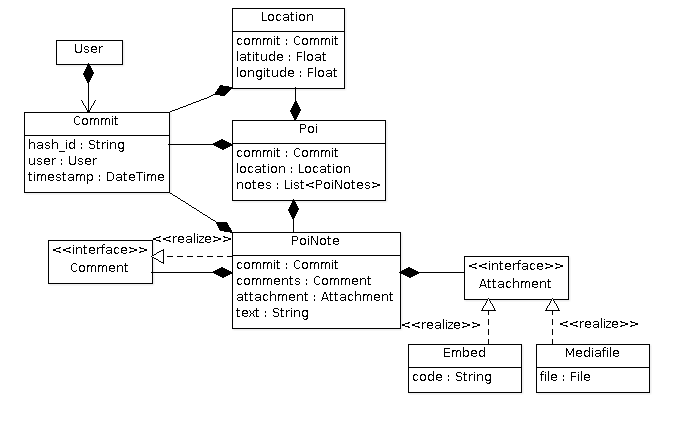
\includegraphics[scale=0.6]{bilder/uml/er_poi.png}
  	  \caption{PoI-Schema}
  \end{figure}
\begin{itemize}[leftmargin=*,noitemsep,topsep=1ex,parsep=0pt,partopsep=0pt]
\item \textbf{Location}: Jeder Markierung auf der Karte ist ein Eintrag in der Tabelle "`locations"' zugeordnet. Alle Entitäten sind direkt oder indirekt mit einem Ort verbunden.
\item \textbf{User}: Anwendungs-Benutzer. In den PoI-Teil-Modell-Entitäten wird der Benutzer über den Commit assoziiert.
\item \textbf{Poi}: Ein Poi besteht aus der Location und mindestens einer PoI-Note.
\item \textbf{PoiNote}: Poi-Beschreibung bzw. -Kommentar in Textform, optional mit einem Multimedia-Anhang (Attachment).
\item \textbf{Embed, Mediafile}: Attachment-Content-Typen.
\item \textbf{Commit}: Jede Änderung der System-Daten (bzw. der daraus resultierende Datenstand), kann über einen Commit referenziert werden. Ein Commit hat einen "`Autor"' und kann aus einem oder mehreren, zu einer Transaktion zusammengefassten Änderungsschritten, bestehen. Commits werden zur Synchronisation von replizierten Benutzer-Kopien mit den System-Masterdaten genutzt. 
\end{itemize}
%\enlargethispage{3\baselineskip} % allow 3 more lines on current page
  \begin{figure}[H]
      \centering
	  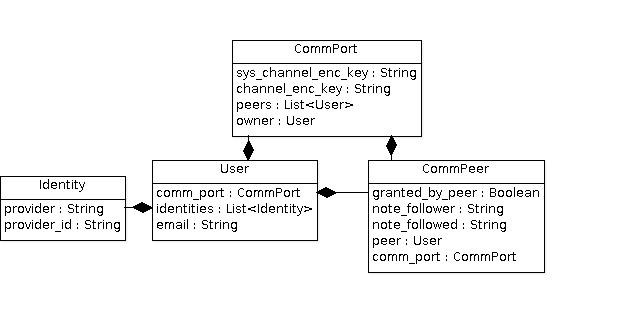
\includegraphics[scale=0.6]{bilder/uml/er_user.png}
  	  \caption{Kommunikations-Schema}
  \end{figure}
\begin{itemize}[leftmargin=*,noitemsep,topsep=1ex,parsep=0pt,partopsep=0pt]
\item \textbf{User}: Anwendungs-Benutzer
\item \textbf{Identity}: Benutzer können auf verschiedene Weise authentisiert werden, z.B. durch lokale Registrierung mit Passwort und Email oder über eine Dritten wie Soziale Netzwerke. Für einen Benutzer können mehrere Autorisierungs-Anbieter mit jeweils einer zugeordneten Identity existieren.
\item \textbf{CommPort}: Darin werden Eigenschaften und Einstellungen der Kommunikations-Schnittstelle eines Benutzer gespeichert.
\item \textbf{CommPeer}: Die Abbildung einer P2P-Beziehung. Benutzer folgen dem CommPort eines anderen Benutzers. Im Feld \texttt{granted\_by\_peer} wird der Autorisierungs/Follow-Status der Beziehung gesetzt. Zusätzlich können beide Benutzer Notizen zum jeweils anderen Benutzer speichern.
\end{itemize}

\subsubsection{Messaging}\label{5_MESSGNG}
Als Implementierung einer synchronen Kommunikation zwischen online-Benutzern wurde für VoyageX die Publish-Subscribe-Messaging-Lösung \texttt{Faye} gewählt, deren Client-Implementierung von allen aktuell verbreiteten Browsern unterstützt wird.\\
Eine alternative Lösung könnte auch mit \texttt{WebRTC} realisiert werden
%, dabei müsste aber die Verwaltung logischer Verbindungen, anders als bei Faye, von Grund auf selbst programmiert werden.
%da es sich , und somit eine 
% Zur Zeit befindet sich aber ein Standard in Entwicklung, der im Falle der Verfügbarkeit in allen Browsern bzw. auf allen Plattformen die erste Wahl wäre, so daß er hier kurz vorgestellt werden soll. Die Kommunikations-Schicht ist bei VoyageX aber soweit geschichtet, so daß ein Wechsel ohne Anpassungen der restlichen Anwendungsfunktionen möglich ist. \\
%In der Rack-Anwendung des Backends wird die Kommunikations-Schnittstelle mittels Gem als Rails-Plugin in einem eigenen Engin gemounted

\paragraph{Web-Real-Time-Communication - WebRTC$^{\textbf{\ref{CMTMYSQL}}}$}
\addtocounter{footnote}{1}%
\footnotetext{\label{CMTMYSQL}\href{http://de.wikipedia.org/wiki/WebRTC}{WebRTC - http://de.wikipedia.org/wiki/WebRTC}; letzter Zugriff: 22.01.2015}
WebRTC ist eine auf Html5 basierende Schnittstellen-Definition, die eine Audio- und Video-Übertragung auf Peer-To-Peer Basis realisiert. Diese API teilt sich in die Bereiche:
\begin{itemize}[leftmargin=*,noitemsep,topsep=1ex,parsep=0pt,partopsep=0pt]
\item Protokolle und Mechanismen zum Aufbau einer Kommunikations-Infrastruktur
\item Zugriff auf die in der plattform-spezifischen Laufzeit-Umgebung verfügbaren Multimedia-Hardware-Komponenten
\end{itemize}
WebRTC ist zwar ein im Draft-Status befindlicher W3C-Standard, wird aber noch nicht von Safari (IOS/MacOS) oder IE unterstützt - für eine plattformübergreifende Kommunikations-Lösung ist WebRTC also noch nicht geeignet.\\ \\
In VoyageX wird allerdings die Hardware-Zugriffs-API der WebRTC für die Aufnahme von Fotos unter Chrome und Firefox verwendet, für andere Browser werden dafür andere, plattform-spezifische Lösungen bereitgestellt.
%es gibt zwar auch einen ansatz atlassian als plugin zu 

\paragraph{Faye}\label{Faye}
Die Plattform-Unabhängigkeit wird im Faye-Client durch die Implementierung des \texttt{Bayeux-Protokolls}$^{\textbf{\ref{CMTBAYX}}}$%
\addtocounter{footnote}{1}%
\footnotetext{\label{CMTBAYX}\href{http://svn.cometd.org/trunk/bayeux/bayeux.html}{Bayeux - http://svn.cometd.org/trunk/bayeux/bayeux.html}; letzter Zugriff: 22.01.2015} erreicht. Bayeux definiert Verbindungs-Verwaltung und Transport-Steuerung für eine Kommunikations-Infrastruktur auf Basis eines Publish-Subscribe-Messaging-Systems, indem zur Sitzungs-Konfiguration Handshake-Nachrichten in Meta-Kanälen ausgetauscht werden. Dadurch können beispielsweise verschiedene Verbindungs- und Transport-Protokoll-Alternativen implementiert werden, so daß der Client je nach Plattform und Technologie-Verfügbareit aus folgenden Kommunikations-Protokollen / -Strategien wählen kann:
	\begin{itemize}
		\item Persistente Verbindungen mit WebSockets
		\item Long-polling via HTTP POST
		\item Cross Origin Resource Sharing
		\item Callback-polling via JSON-P
	\end{itemize}
%TODO: Akku-Verbrauch bei mobilen Clients analysieren
%Für die Faye-Lösung spricht aber auch die bereits vollständig implementierte Messaging-Kommunikations-Infrastruktur und die damit verbundene Verminderung des eigenen Programmier-Aufwandes.\\
Die Publish-Subscribe-Funktionen können auch von einer Anwendung "`out-of-the-box"' genutzt werden, indem die Wahl eines beliebigen Namens ausreicht, um einen Kanal für den Nachrichten-Austausch zu definieren, und diesen über Client-API nutzen zu können:
\lstset{language=JavaScript}
\begin{lstlisting}[frame=single,xleftmargin=0pt,numbers=none]
publish "/kanalXYZ" "hello world message"
subscribe "/kanalXYZ"
\end{lstlisting}
Die Kommunikations-Infrastruktur wird von Faye mit einer Client-Server-Architektur realisiert. Frei verfügbare Implementierungen des Faye-Servers gibt es für \texttt{Rack} und \texttt{Node.js}$^{\textbf{\ref{CMTNODEJS}}}$%
\addtocounter{footnote}{1}%
\footnotetext{\label{CMTNODEJS}\href{https://nodejs.org/}{Node.js - https://nodejs.org/}; letzter Zugriff: 22.05.2015} - in Web-Browser-Clients wird eine freie Javascript-Bibliothek genutzt.
Die Server-Komponente wird bei Rack, wie in \ref{FAYERAILS} beschrieben, als Middleware in das Backend integriert.

%%%%%%%%%%%%%%%%%%%%%%%%%%%%%%%%%%%%%%%%%%%%%%%%%%%%%%%%%%%%%%
% Frontend
%%%%%%%%%%%%%%%%%%%%%%%%%%%%%%%%%%%%%%%%%%%%%%%%%%%%%%%%%%%%%%
\subsection{Frontend}\label{5_FE}

\subsubsection{Coffee-Script}
Die Anwendungs-Logik des Frontends von VoyageX ist in \texttt{CoffeeScript}$^{\textbf{\ref{CMTBAYX}}}$%
\addtocounter{footnote}{1}%
\footnotetext{\label{CMTBAYX}\href{http://de.wikipedia.org/wiki/CoffeeScript}{CoffeeScript - http://de.wikipedia.org/wiki/CoffeeScript}; letzter Zugriff: 22.01.2015} geschrieben, welches im Backend vom Ruby-Gem \texttt{coffee-rails} in JavaScript transkompiliert wird.\\
Bei zunehmender Anwendungs-Komplexität ist es schwierig, übersichtlichen Programm-Code mit gewöhnlichem JavaScript zu schreiben. Ein wesentlicher Nutzen von CoffeeScript ist die Verbesserung der Lesbarkeit von Javascript-Code. Dies wird durch eine saubere objektorientierte Syntax und durch weitere Syntactic-Sugar-Features und Utilitiy-Methoden erreicht. Ein weiterer Vorteil ist die Erkennung von Syntaxfehlern beim Transkompilieren$^{\textbf{\ref{CMTBAYX}}}$%
\addtocounter{footnote}{1}%
\footnotetext{\label{CMTBAYX}Compiler bieten durch statische Code-Analyse generell gute Möglichkeiten zur Fehlererkennung.}. 

\subsubsection{Anforderungen an den Client / Browser}\label{4_ACB}
%VoyageX soll als Single Page (Web-)Application (SPA) realisiert und kann 
VoyageX soll zwar mit verschiedenen Browsern auf unterschiedlichen Plattformen / Betriebssystemen genutzt werden können, bei der angestrebten Plattformunabhängigkeit gibt es aber dennoch Einschränkungen. Die volle Funktionalität kann auf mobilen Endgeräten nur für den Chrome-Browser (>= 42) unter Android, und auf Desktop-Rechnern für den Chrome-Browser (>= 39) unter Linux garantiert werden.

\paragraph{Html5}
Html5$^{\textbf{\ref{HTML5}}}$%
% footnote
\addtocounter{footnote}{1}%
\footnotetext{\label{HTML5}\href{http://www.w3.org/blog/news/archives/4167}{Html5 - http://www.w3.org/blog/news/archives/4167}; letzter Zugriff: 01.03.2015}
ist die fünfte Version des Html Standards. Im Vergleich zu Html4 wurde unter anderem die Multimedia-Schnittstelle wesentlich erweitert, um auch die Nutzung neuer Hardware-Technologien aus diesem Bereich in einer Web-Anwendung anbieten zu können. VoyageX setzt HTML5-fähige Browser-Versionen voraus. 
	\begin{table}[H]
  		\begin{adjustwidth}{-1.5cm}{1.5cm}
		\centering
		\begin{tabulary}{20cm}{C}
	  		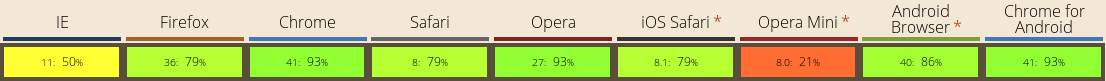
\includegraphics[scale=0.6]{bilder/screenshots/caniuse_html5.png}\\ 
				\ccLogo\ 
				\begingroup
    				\fontsize{8pt}{12pt}\selectfont
    				\href{http://caniuse.com/\#search=html5}{Can I use}; Lizenz: \href{http://creativecommons.org/licenses/by-nc/3.0/}{CC BY-NC 3.0} 
				\endgroup\\ 
	  		Noch nicht alle Features von Html5 werden von allen Browsern unterstützt.
		\end{tabulary}
  		\end{adjustwidth}
	\end{table}

\paragraph{Web Storage}
Web Storage war ursprünglich Teil der Html5 Spezifikation, ist aber mittlerweile ein eigener Standard$^{\textbf{\ref{WEBSTRG}}}$%
% footnote
\addtocounter{footnote}{1}%
\footnotetext{\label{WEBSTRG}\href{http://www.w3.org/TR/webstorage/}{Web Storage - http://www.w3.org/TR/webstorage/}; letzter Zugriff: 01.03.2015}
. Von den beiden Teil-Komponenten Session Storage und Local Storage nutzt VoyageX letztere zum Speichern von Anwendungsdaten für den Offline-Betrieb.
	\begin{table}[H]
  		\begin{adjustwidth}{-1.5cm}{1.5cm}
		\centering
		\begin{tabulary}{20cm}{C}
	  		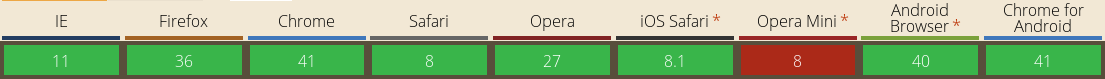
\includegraphics[scale=0.6]{bilder/screenshots/caniuse_webstorage.png}\\ 
				\ccLogo\ 
				\begingroup
    				\fontsize{8pt}{12pt}\selectfont
    				\href{http://caniuse.com/\#search=webstorage}{Can I use}; Lizenz: \href{http://creativecommons.org/licenses/by-nc/3.0/}{CC BY-NC 3.0} 
				\endgroup
		\end{tabulary}
  		\end{adjustwidth}
	\end{table}

\paragraph{Application Cache}
Im Application Cache kann die Anwendung Quelldateien, wie Javascript und CSS-Stylesheets, Bild-Dateien oder andere statischen Anwendungskomponenten für einen späteren Gebrauch im Offline-Modus vom Browser speichern. Die zu speichernden Komponenten werden dabei in einer Manifest-Datei$^{\textbf{\ref{CACMAN}}}$%
% footnote
\addtocounter{footnote}{1}%
\footnotetext{\label{CACMAN}\href{http://en.wikipedia.org/wiki/Cache_manifest_in_HTML5}{Cache Manifest - http://en.wikipedia.org/wiki/Cache\_manifest\_in\_HTML5}; letzter Zugriff: 01.03.2015}
notiert. 
	\begin{table}[H]
  		\begin{adjustwidth}{-1.5cm}{1.5cm}
		\centering
		\begin{tabulary}{20cm}{C}
	  		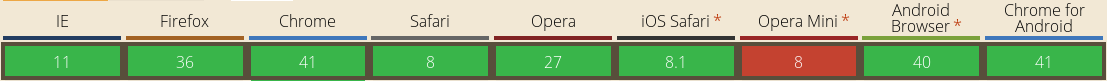
\includegraphics[scale=0.6]{bilder/screenshots/caniuse_appcache.png}\\ 
				\ccLogo\ 
				\begingroup
    				\fontsize{8pt}{12pt}\selectfont
    				\href{http://caniuse.com/\#search=Application\%20Cache}{Can I use}; Lizenz: \href{http://creativecommons.org/licenses/by-nc/3.0/}{CC BY-NC 3.0} 
				\endgroup
		\end{tabulary}
  		\end{adjustwidth}
	\end{table}

\paragraph{File API}
Die File-API ist eine von Html5 definierte Javascript-Schnittstelle die es einer Anwendung erlaubt, Dateien lokal zu speichern. Im Gegensatz zum \texttt{localStorage}, welches nur das Speichern von Zeichenketten ermöglicht, steht mit dieser API ein echtes Filesystem zur Verfügung. Ein entscheidender Vorteil gegenüber dem localStorage ist es, daß die maximale Speicherkapazität nach oben nicht durch 5 MB$^{\textbf{\ref{CMT5MBLIM}}}$%
\addtocounter{footnote}{1}%
\footnotetext{\label{CMT5MBLIM}Dieser Wert kann je nach Browser variieren.} beschränkt ist, sondern vom Benutzer festgelegt wird. Daten können somit auch im Gigabyte-Bereich auf dem Client abgelegt werden.
	\begin{table}[H]
  		\begin{adjustwidth}{-1.5cm}{1.5cm}
		\centering
		\begin{tabulary}{20cm}{C}
          	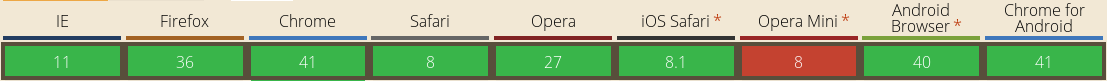
\includegraphics[scale=0.6]{bilder/screenshots/caniuse_fileapi.png}\\ 
				\ccLogo\ 
				\begingroup
    				\fontsize{8pt}{12pt}\selectfont
    				\href{http://caniuse.com/\#search=file\%20api}{Can I use}; Lizenz: \href{http://creativecommons.org/licenses/by-nc/3.0/}{CC BY-NC 3.0} 
				\endgroup
		\end{tabulary}
  		\end{adjustwidth}
	\end{table}

\paragraph{Media Providers}
Mit \texttt{MediaSource} und \texttt{MediaStream} sind in Html5 Javascript-Schnittstellen definiert, die das Aufnehmen und Abspielen von Audio bzw. Videodateien ermöglichen. Insbesondere können auch Fotos in Form von Video-Snapshots aufgenommen werden.
	\begin{table}[H]
  		\begin{adjustwidth}{-1.5cm}{1.5cm}
		\centering
		\begin{tabulary}{20cm}{C}
          	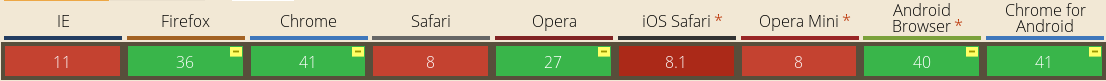
\includegraphics[scale=0.6]{bilder/screenshots/caniuse_mediastream.png}\\ 
				\ccLogo\ 
				\begingroup
    				\fontsize{8pt}{12pt}\selectfont
    				\href{http://caniuse.com/\#search=Media\%20Stream}{Can I use}; Lizenz: \href{http://creativecommons.org/licenses/by-nc/3.0/}{CC BY-NC 3.0} 
				\endgroup
		\end{tabulary}
  		\end{adjustwidth}
	\end{table}

\subsubsection{Datenspeicherung und Entitäten}\label{5_DSE}
Bei Single-Page-Interface Webanwendungen, werden die Pattern-Komponenten \texttt{View} und \texttt{PresentationModel}$^{\textbf{\ref{CMTPRESMD}}}$%
\addtocounter{footnote}{1}%
\footnotetext{\label{CMTPRESMD}\href{http://martinfowler.com/eaaDev/PresentationModel.html}{PresentationModel - http://martinfowler.com/eaaDev/PresentationModel.html}; letzter Zugriff: 22.05.2015} clientseitig implementiert. Die \texttt{Model}-Komponenten befinden sich am Backend-Server, wobei die Daten dann über \texttt{Databinding} in die View gelesen bzw. ins Model geschrieben werden$^{\textbf{\ref{CMTMVVM}}}$%
\addtocounter{footnote}{1}%
\footnotetext{\label{CMTMVVM}\href{http://de.wikipedia.org/wiki/Model\_View\_ViewModel}{MVVM - http://de.wikipedia.org/wiki/Model\_View\_ViewModel}; letzter Zugriff: 22.04.2015}. Nach Daten-Änderungen wird dann eine aktualisierte GUI-Ansicht mit Javascript aus Html-Templates, CSS und den Daten generiert. Bei einer offline-fähigen Anwendung wie VoyageX werden aber auch die \texttt{Model}-Komponenten clientseitig implementiert, da hier eine eigene, von einer Netzwerk-Verbindung unabhängige Persistenz-Verwaltung benötigt wird.\\ \\
Folgende (replizierte) Daten müssen für eine Nutzung der Anwendung bei fehlender Netzwerkverbindung lokal gespeichert und geändert werden können:
\begin{itemize}[leftmargin=*,noitemsep,topsep=1ex,parsep=0pt,partopsep=0pt]
\item PoI-Daten, die für den lokalen Benutzer relevant sind. Die Relevanz wird dabei durch die vom Benutzer festgelegte geographische Begrenzung des bearbeitbaren Kartenauschnitts entschieden. 
\item Daten über entfernte Benutzer, zu denen eine Kontakt-Beziehung besteht.
\item PoI-Daten die der Benutzer im Offline-Modus selbst erstellt.
\end{itemize}
Für das Speichern und die Verwaltung von Daten im Client-Browser gibt es mehrere Möglichkeiten die sich nach Kapazität und Plattform-Verfügbarkeit unterscheiden.

\enlargethispage{3\baselineskip} % allow 3 more lines on current page
\paragraph{localStorage (Webstorage), IndexedDB, WebSQL und File-API}
	\begin{table}[H]
		\centering
		\begin{tabulary}{\columnwidth}{|L|C|C|C|C|}
		\hline
			& \textbf{Webstorage} & \textbf{IndexedDB$^{\textbf{\ref{CMTIDXDB}}}$} & \textbf{WebSQL} & \textbf{File-API} \\ \hline
%						  1   2   3	  4   5   6   7   8   9   10  11  12  13  14  15		
			W3C-Recommendation     & Y & Y & N & N \\ \hline
			Plattform     & IE,FF,CH,SA,OP & FF,CH,OP & CH,SA,OP & IE,FF,CH,SA,OP \\ \hline
			Größen-Limit     & 5-10MB & 10\%HD & - & - \\ \hline
			Storage-Type    & Key-Value & ObjectStore & Relational & Filesystem \\ \hline
		\end{tabulary}
		\caption{Client-seitige Persistenz-APIs}
	\end{table}
\addtocounter{footnote}{1}%
\footnotetext{\label{CMTIDXDB}\href{http://de.wikipedia.org/wiki/Indexed\_Database\_API}{IndexedDB - http://de.wikipedia.org/wiki/Indexed\_Database\_API}; letzter Zugriff: 22.01.2015}
Als kommender Standard und wegen der Speicherkapazität und den erweiterten Such- bzw. Abfrage-Funktionen wäre \texttt{IndexedDB} eine gute Wahl, allerdings fehlt dafür noch die Unterstützung auf wichtigen Plattformen. 
	\begin{table}[H]
  		\begin{adjustwidth}{-1.5cm}{1.5cm}
		\centering
		\begin{tabulary}{20cm}{C}
	  		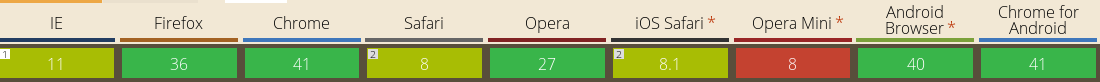
\includegraphics[scale=0.6]{bilder/screenshots/caniuse_indexeddb.png}\\
				\ccLogo\ 
				\begingroup
    				\fontsize{8pt}{12pt}\selectfont
    				\href{http://caniuse.com/\#search=IndexedDB}{Can I use}; Lizenz: \href{http://creativecommons.org/licenses/by-nc/3.0/}{CC BY-NC 3.0} 
				\endgroup
		\end{tabulary}
  		\end{adjustwidth}
	\end{table}
\noindent
Aus diesem Grund wird in VoyageX eine Kombination aus \texttt{localStorage} und \texttt{File-API} für die client-seitige Persistenz der Anwendungsdaten gewählt. Die Persistenz-Schnittstelle der CoffeeScript-Klasse \texttt{StorageController} von VoyageX erlaubt allerdings einen aufwandsarmen späteren Austausch der gewählten Implementierung.

\paragraph{Entitäten}
Viele Entitäten des im Backend verwendeten, relationalen ER-Modells werden auf Client-Seite mit JSON-Datenstrukturen nachgebildet. Dabei werden die JSON-Objekte mit einem \texttt{Schlüssel} entweder einzeln (Id im Schlüssel) oder als Liste (Id im JSON-Objekt) im localStorage gespeichert.
\lstset{language=JavaScript}
\begin{lstlisting}[frame=single,xleftmargin=0pt,numbers=none,caption={Lesen und Speichern von JSON-Objekten mit localStorage},captionpos=b]
key = 'comm.locations'
locations = JSON.parse(localStorage.getItem(key))
...
localStorage.setItem key, JSON.stringify(locations)
\end{lstlisting}
%Die Unterscheidung hängt damit zusammen, daß beim Auslesen die gesamte Zeichenkette in ein JSON-Objekt, und beim Speichern wieder in eine Zeichenkette konvertiert wird. Sind viele Objekte, große Datenmengen oder dynamische Sub-Listen pro Eintrag zu erwarten, dann wird jede Entität einzeln gespeichert - bei wenigen Objekten, kleinen Datenmengen oder Sub-Listen-freien Entitäten wird eine Liste verwendet. Dieses Modell ist aber willkürlich und sollte noch untersucht werden.

\subparagraph{User:}
User werden in einer Liste mit dem Schlüssel \texttt{comm.users} gespeichert.
\lstset{language=JavaScript}
\begin{lstlisting}[frame=single,xleftmargin=0pt,numbers=none,caption={users.json},captionpos=b]
{
  "264":{"username":"homer","foto":{...},"peerPort":{...},...},
  "391":{"username":"marge","foto":{...},"peerPort":{...},...}
}
\end{lstlisting}

\subparagraph{Location:}
Locations werden in einer Liste mit dem Schlüssel \texttt{comm.locations} gespeichert.
\lstset{language=JavaScript}
\begin{lstlisting}[frame=single,xleftmargin=0pt,numbers=none,caption={locations.json},captionpos=b]
{
  "4276":{"lat":52.4980698,"lng":13.416569,"address":"Bergstr. 3"},
  "4285":{"lat":52.4639426,"lng":13.3728893,"address":"Urbanstr. 6"}
}
\end{lstlisting}

\subparagraph{Poi:}
Pois werden einzeln gespeichert, z.B. PoI 36 mit Schlüssel \texttt{comm.poi.36}
\lstset{language=JavaScript}
\begin{lstlisting}[frame=single,xleftmargin=0pt,numbers=none,caption={poi.json},captionpos=b]
{
  "locationId":4308,
  "notes":[
    {"id":65, "text":"...","attachment":{...}}
   ],
   "userId":264
 }
\end{lstlisting}

%\subsubsection{Internationalisierung}
%Internationalisierung ist besonders bei einer Geo-basierten Webanwendungen sinnvoll, da die Exsitenz von Interaktions-Einschränkungen durch Sprach-Barrieren im Widerspruch zur unbegrenzten Verfügbarkeit des Kartenmaterials stehen. Zur Unterstützung mehrsprachiger Views werden von VoyageX die Standard Lokalisierungs- und Internationalisierungs-Funktionen von RoR genutzt. Dementsprechend muß ein Benutzer für
%den Wechsel zu einer andern Sprache online sein.  

\subsubsection{Bibliotheken}
Für VoyageX werden freie Bibliotheken Dritter (3$^{rd}$-Party Libraries) eingesetzt, welche vielfach getestete und bewährte Lösungs-Implementierungen benötigter Funktionen bereitstellen. Neben der Qualitäts-Sicherung ist die Verminderung des eigenen Programmieraufwandes ein starkes Argument für den Einsatz von externen
Modulen.

\paragraph{jQuery}
jQuery ist eine Javascript-Bibliothek die zahlreiche Funktionen für die Implementierung einer \texttt{Rich-Internet-Anwendung (RIA)}$^{\textbf{\ref{CMTRICHIA}}}$%
\addtocounter{footnote}{1}%
\footnotetext{\label{CMTRICHIA}\href{http://de.wikipedia.org/wiki/Rich\_Internet\_Application}{RIAs sind Webanwendungen mit einer hoch-interaktiven Benutzeroberfläche - http://de.wikipedia.org/wiki/Rich\_Internet\_Application}; letzter Zugriff: 22.04.2015} bereitstellt:
	\begin{itemize}
		\item DOM: Manipulation und Interaktion mit Animationen und Ereignis-Notifikation
		\item Ajax
		\item Plugin-Schnittstelle für Implementierung zusätzlicher Funktionen
	\end{itemize}
Mit jQuery ist es denkbar einfach DOM-Elemente über einen \texttt{\$('...')-Selector} auszuwählen, und eingebaute jQuery-Funktionen oder eigene Funktionen darauf anzuwenden. Im folgenden Beispiel-Snippet wird im Chat-Popup zur Nachricht 143 gescrollt.
\lstset{language=JavaScript}
\begin{lstlisting}[frame=single,xleftmargin=0pt,numbers=none]
$('#p2pChat').closest('.leaflet-popup').scrollTop(
		$('#p2p-msg-143').offset().top
  )
\end{lstlisting}

\paragraph{LeafletJS}
{LeafletJS$^{\textbf{\ref{FN_LEAFL}}}$}\label{LEAFL}
% @see 3 - Web-Mapping-Apis
ist eine freie Map-Viewer-Javascript-Bibliothek zur Einbindung interaktiver Karten in eine Html-Seite.
Es können beliebige Kartenprojektionen dargestellt werden (neben geographischen Karten beispielsweise auch Sternenkarten), solange ein Tile-Service für die benötigten Karten-Kachel-Bilder angegeben werden kann.
%Als Karteninhalt kann dabei jede Form der Projektion gewählt werden, die dann über einen konfigurierbaren Tile-Map-Service zur Darstellung gebracht wird.
Neben dem Laden der Kacheln (vgl. Abschnitt \ref{MAPVIEWER}) bietet die Bibliothek aber auch Schnittstellen für eine Vielzahl weiterer Funktionen zur Kartenbearbeitung, wie beispielsweise das setzen von Markierungen und deren Verknüpfung mit Popups, oder das Hinzufügen von graphischen Elementen wie Linien oder Polygone in die Kartenansicht. 
Durch seine flexible Plugin-Schnittstelle und ein entsprechend großes Angebot frei verfügbarer Plugins eignet sich LeafletJS sehr gut für die Realisierung der geforderten Funktions-Anforderung für VoyageX.

\paragraph{Faye Client}
Zur serverseitigen Kommunikations-Schnittstelle (vgl. Abschnitt \ref{FAYERAILS}) wird mit dem Faye Paket
eine Messaging-Client-Javascript-Bibliothek augeliefert, die den Nachrichten-Austausch mit dem Backend organisiert. Nachdem der Client instanziert wurde stehen 3 Funktionen für den Aufbau einer eigenen Kommunikations-Lösung zur Verfügung:\\
\lstset{language=JavaScript}
\begin{lstlisting}[frame=single,numbers=none,xleftmargin=0pt,caption={API des Faye-Clients},captionpos=b]
    client = new Faye.Client(document.location.origin+'/comm')

    client.subscribe channel, messageCallBack
    client.unsubscribe channel

    client.publish channel, message
\end{lstlisting}

\paragraph{Verbindungs-Zustands-Überwachung}
Bestimmte Funktionen von VoyageX sollen bei jedem Verbindungszustand verfügbar sein, allerdings
wird das Verhalten der Anwendung von diesem Zustand beeinflusst. So werden Chat-Nachrichten im Offline-Zustand zwar bis zum
späteren Transport gepuffert, ohne daß der Benutzer selbst das Versenden erneut veranlassen muss, allerdings sollte der Benutzer dennoch darauf hingewiesen werden, daß die Aktion nicht unmittelbar ausgeführt werden kann, da er sonst vielleicht eine unmittelbare Antwort vom Empfänger erwarten würde. Aus diesem Grund wird der Verbindungszustand in VoyageX jederzeit durch die Farbgebung der Menu-Leiste widergespiegelt (grün: online, rot: offline).\\% um keine falschen Annahmen zu fördern.\\
Es gibt bei VoyageX 3 verschiedene Online-Zustände:
	\begin{itemize}
		\item Plattform: Wenn der Rechner des Benutzers bzw. der Browser ist können Kartenkachel geladen werden. Zustand wird über navigator.Online ermittelt.
		\item Backend: Wenn eine Verbindung zum Backend besteht können Daten synchronisiert werden. Zustand wird über eigene "`ping"'-Funktion  überwacht (falls Plattform online ist).
		\item Faye-Server: Wenn eine Verbindung zum Kommunikations-Server besteht können Echtzeit-Nachrichten ausgetauscht werden. Zustand wird vom Faye-Client per Websocket-Status überwacht.
	\end{itemize}


\subsubsection{Views}
%hinweis: onlinestatus grün pder rot
In VoyageX gibt es 3 Haupt-Ansichten, zwischen denen über das Haupt-Menu gewechselt werden kann:
\begin{itemize}[leftmargin=*,noitemsep,topsep=1ex,parsep=0pt,partopsep=0pt]
\item \textbf{Konferenz}: Diese Ansicht wird für die Gruppenkommuniation genutzt und zeigt ein 2-teiliges Chat-Fenster: Im oberen Bereich werden die Nachrichten angezeigt, im unteren Bereich kann der Benutzer den Text für eigene Nachrichten eingeben und per Eingabetaste absenden. 
\item \textbf{Karte}: In dieser Ansicht werden die Karte, sowie Navigations- und Steuerungs-Elemente angezeigt.
\item \textbf{Home}: In der Home-Ansicht befinden sich die Eingabe- und Steuerungs-Elemente zur Verwaltung der Benutzer- und Kontakt-Daten.
\end{itemize}
	
	\begin{table}[H]
  		\begin{adjustwidth}{-0.3cm}{0.3cm}
		\centering
		\begin{tabulary}{\columnwidth}{C >{\centering}m{1cm} C >{\centering}m{1cm} C}
			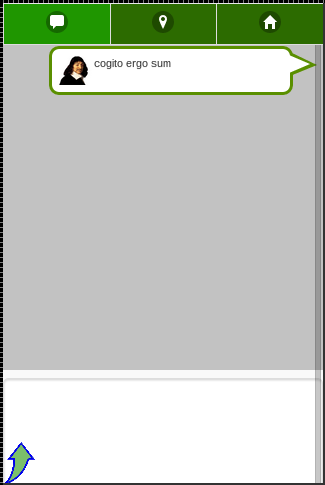
\includegraphics[scale=0.5]{bilder/screenshots/conference.png} & & 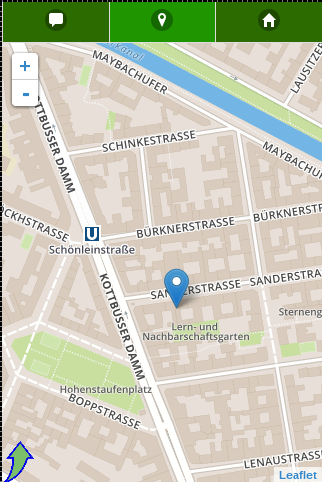
\includegraphics[scale=0.5]{bilder/screenshots/map.png} & & 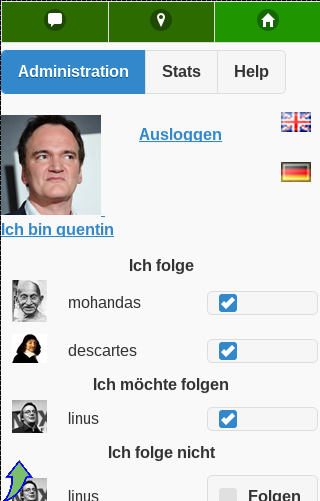
\includegraphics[scale=0.5]{bilder/screenshots/home.png} \\
			Conference & & Map & & Home
		\end{tabulary}
  		\end{adjustwidth}
	\end{table}
\noindent
Ein Klick auf den grünen Pfeil links unten öffnet ein Kontext-Navigations-Fenster, das aus 3 Unter-Ansichten besteht.
\enlargethispage{3\baselineskip} % allow 3 more lines on current page
Jede dieser Ansichten beinhaltet Links zu Punkten auf der Karte und ermöglicht damit eine schnelle Kontext-bezogene Navigation:
\begin{itemize}[leftmargin=*,noitemsep,topsep=1ex,parsep=0pt,partopsep=0pt]
\item \textbf{Points-Of-Interest}: Hier werden alle PoIs im angegebenen Umkreis angezeigt. 
\item \textbf{Bookmarked Locations}: Hier werden alle PoIs und Locations angezeigt, für die der Benutzer
ein Lesezeichen eingetragen hat.
\item \textbf{People Of Interest}: Hier werden alle entfernten Benutzer angezeigt, mit denen der lokale Benutzer eine Kontakt-Beziehung hält.
\end{itemize}
	
	\begin{table}[H]
  		\begin{adjustwidth}{-0.3cm}{0.3cm}
		\centering
		\begin{tabulary}{\columnwidth}{C >{\centering}m{1cm} C >{\centering}m{1cm} C}
			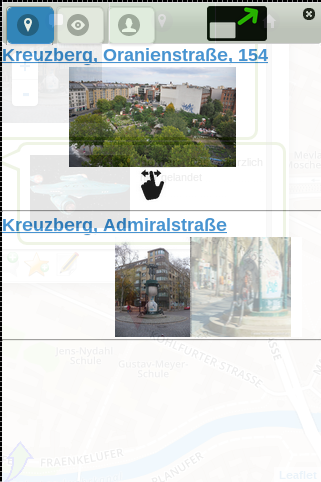
\includegraphics[scale=0.5]{bilder/screenshots/context_nav_pois.png} & & 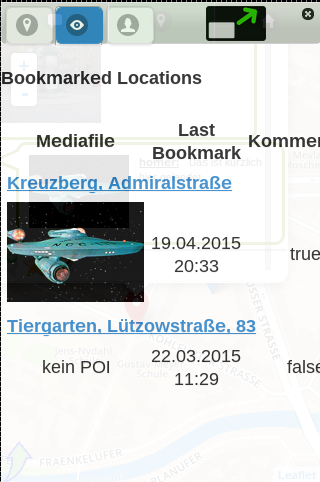
\includegraphics[scale=0.5]{bilder/screenshots/context_nav_bookmarks.png} & & 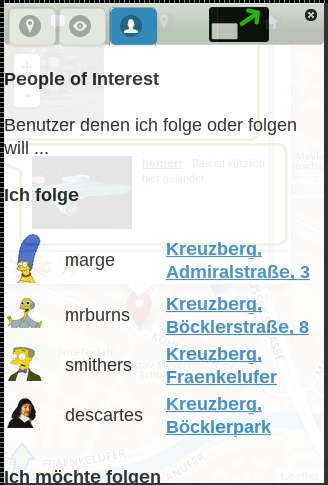
\includegraphics[scale=0.5]{bilder/screenshots/context_nav_contacts.png} \\
			Points of Interest & & Bookmarks & & People of Interest
		\end{tabulary}
  		\end{adjustwidth}
	\end{table}

\subsubsection{Registrierung \& Login}

\paragraph{Registrierung}
Zur vollen Nutzung der Anwendung muß ein Benutzer vom System authentisiert sein. Es gibt 2 Möglichkeiten sich 
zu registrieren:
\begin{itemize}
	\item Registrierung mit Email-Adresse und Passwort
	\item Registrierung mit einem Konto eines sozialen Netzwerks wie Facebook oder Twitter
\end{itemize}
\noindent Bei der Registrierung mit einem Passwort muss der Benutzer die Möglichkeit haben ein neues Passwort anzufordern wenn er nicht angemeldet ist.
%Das gilt nur bei einer Registrieung mit Email-Adresse und Passwort.

\paragraph{Login}
Eine Sitzung ist aus Sicherheitsgründen zeitlich begrenzt. Da sich ein Benutzer von jedem beliebigen Rechner einloggen kann muss verhindert werden, daß eine andere Person die authentisierte Sitzung eines Benutzers fortführt, falls letzterer die Sitzung nicht selbst durch eine aktive Abmeldung vom System beendet hat. 

\paragraph{Quick Registration}
Um es neuen Benutzern zu erleichtern das funktionale Angebot von VoyageX kennenzulernen und dennoch die registrierten 
Mitglieder der Community vor Störungen durch Aktivitäten unbekannter Nutzer zu schützen, wird eine Quick Registration angeboten, die eine volatile kollaborative Session ermöglicht (siehe auch \cite[S. 72ff.]{SCLU:PFCMI}).
Bei dieser Form der Registrierung ist der Funktionsumfang der Anwendung für den Benutzer allerdings das Lesen von Einträgen beschränkt.


\subsubsection{Community Support}
%\paragraph{Gruppen}
%TODO - Dieses Feature ist noch nicht programmiert - macht es Sinn? + wenn der Aufwand zu groß ist dann als TODO.\\
%Gruppen können nur von Benutzern mit entsprechender Berechtigung angelegt werden. Um einer Gruppe beitreten zu können
%benötigt ein Benutzer eine Einladung. Alle offenen Einladungen werden als Link in der Verwaltungs-Ansicht angezeigt.\\
%Alle Interaktions-Funktionen der Anwendung sind auf die Mitglieder jener Gruppen beschränkt, für welche ein Benutzer eine Mitgliedschaft besitzt. Die Interaktion mit anderen Gruppenmitgliedern ist aber nicht verpflichtend - d.h. daß man anderen Gruppenmitgliedern nicht folgen muß.\\
%mit Gruppen macht auch eine user-gallery (siehe auch \cite[S. 72ff.]{SCLU:PFCMI}) mehr sinn - was bringt es alle mitglieder des gesamten systems zu sehen?
%(anders wenn bei der user-gallery interessen berücksichtigt werden die der benutzer irgendwo festgelehgt hat.)\\
%Mögliche sinnvolle Erweiterung: Jede Gruppe hat ihre eigenen PoIs.
%wenn ein poiu in 2 gruppen vorkommt muss man eine auswahl treffen, allerdings wird die ja auch in photonav angezeigt -serh komplex. etwas weniger komplex - alle haben poi - erster eintrag bei allen angezeigt aber die darber nur aus der gruppe.

\paragraph{Avatare}
Durch die Einführung von Avataren wird es für die Benutzer einfacher persönliche Kontakte auszuwählen und einen Überblick über ausgewählten Interaktionspartner zu wahren (siehe auch \cite[S. 97ff.]{SCLU:PFCMI}). Jeder Benutzer kann ein Bild (Foto oder Cartoon) wählen, mit dem seine Urheberschaft von Einträgen oder ihm zugeordnete entfernte Peer-Marker für andere Benutzer visuell "`signiert"' werden.
%welches seine alle seine Beiträge und seinen Marker, sowie seine Präsenz in allen Listen schmückt. Jeder Benutzer hat eine Homebase.
%Jeder Benutzer hat mindestens eine Gruppe. und somit eine Zuordnung für andere Benutzer erleichtert wird.

\paragraph{Buddy List}
In VoyageX wählt man Kontakte, an denen man interessiert ist, über die "`Folgen"'-Beziehung.
%von benutzern aus diesen
%gruppen erhält man benachrichtigungen - soweit man dazu berechtigt ist.
%eine der buddy-list bvergleichbare liste wäre dann die liste der benutzer denen ich folgen will und darf, %erweitert um die liste der benutzer denen ich folgenwill aber noch nicht darf.


%\subsubsection{Verwendete Standards, 3rd Party Libs}
%\paragraph{Omniauth}
%omniauth ist ein rails gem das konfigurierbare authentisierungsmechanismen(strategien in omniauth) in form von plugins für viele verbreitete provider(facebook, twitter, ...) oder standards(ldap,..) bietet. fr neue provider können
%neue  strategie-plugins geschrieben werden die ohne änderung des anwendungs-codes eingebunden werden können.

%\paragraph{Avatare}
%zur verinfachung der avatar-einbindung wird die per email-addtesse defieierte bindung von gravatar angeboten - 
%falls der benutzer kein gravata-acount hat wird ein comic-ähnliches bold von einem japanischen hersteller gewäjlt
\subsubsection{Initialisierung des Clients}
Mit dem Aufruf des Konstruktors der Coffee-Script-Klasse \texttt{VoyageX.Main} wird die Anwendung auf Client -Seite gestartet.   
\lstset{language=JavaScript}
\begin{lstlisting}[frame=single,xleftmargin=0pt,numbers=none,label={lst:CL_ClientInit}]
new VoyageX.Main(...) 
\end{lstlisting}
Die Initialisierung erfolgt in mehreren Stufen, da einzelne benötigte Module nur asynchron initialisiert werden können, und der Client erst auf einen "`Ready-Callback"' warten muss bevor weitere, davon abhängige Komponenten initialisiert werden. 
%\vspace{2ex}
  \begin{figure}[H]
      \centering
	  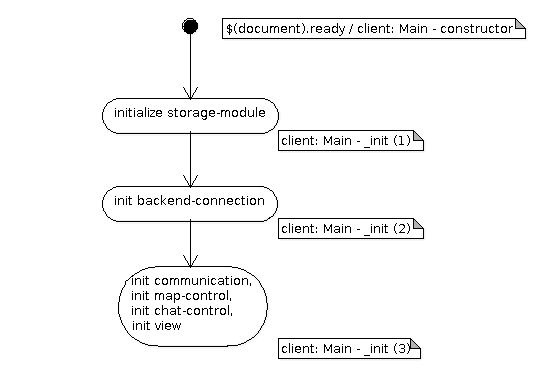
\includegraphics[scale=0.5]{bilder/uml/initClient.png}
  	  \caption{Initialisierung des Clients}
  	  \label{fig:CLIENT_INIT}
  \end{figure}
%%%%%%%%%%%%%%%%%%%%%%%%%%%%%%%%%%%%%%%%%%%%%%%%%%%%%%%%%%%%%%
% Kartenbearbeitung
%%%%%%%%%%%%%%%%%%%%%%%%%%%%%%%%%%%%%%%%%%%%%%%%%%%%%%%%%%%%%%
\subsection{Kartenbearbeitung}\label{5_KARBE}

\subsubsection{Initialisierung der Kartenansicht}\label{5_DARS_KART}
%Die Karten-Ansicht wird mit dem Map-Viewer von LeafletJS initialisiert.
Für die Initialisierung der Karten-Darstellung mit dem LeafletJS-Map-Viewer muß im Html-Quelltext der Seite zunächst ein mit einem frei wählbaren id-Attribut gekennzeichnetes Html-\texttt{div}-Element bereitgestellt werden, welches von Leaflet für die Einbindung der Karte genutzt werden kann.
\lstset{language=Html5}
\begin{lstlisting}[frame=single,numbers=none,xleftmargin=0pt]
<div id="map"></div>
\end{lstlisting}
Mit einem JSON-Objekt (im folgenden Snippet \texttt{mapOptions}) können dann weitere Konfigurations-Parameter übergeben werden, wobei die Parameter \texttt{center} (Kartenmittelpunkt) und \texttt{zoom} (Auflösung) obligatorisch für die Darstellung eines Kartenausschnittes in einem vorgegebenen Maßstab sind. In VoyageX wird beispielsweise
initiial das Zoom-Level 16 eingestellt und die Karte um die letzte bekannte Position des Benutzers zentriert.
%nach erfolgter Positions-Bestimmung des Clients durch die Browser-API-Funktion "`navigator.geolocation.getCurrentPosition"` um die aktuelle Position des Endgerätes zentriert.\\
\lstset{language=JavaScript}
\begin{lstlisting}[frame=single,xleftmargin=0pt,caption={Initialisierung der Karte in einer Haml-Datei},captionpos=b,label={lst:CL_MapInit}]
= javascript_tag do
  ...
  var tileLayer = new L.TileLayer.Functional(VoyageX.MapControl.drawTile, ...)
  var mapOptions = { center: new L.LatLng(#{@lat}, #{@lng}),
   				   	 zooms: [1,2,...,16],
   				   	 zoom: 16,
   				   	 subdomains: ['a'],
   				   	 access_token: 'pk.eyJ1I...ZiG5HGi5JAb64G1K-jA',
   				   	 layers: [tileLayer] }
  new L.Map('map', mapOptions)
\end{lstlisting} \vspace{0.8cm}
\noindent Wie in \ref{LEAFL} bereits beschrieben, macht Leaflet keine Vorgaben zum Darstellungs-Inhalt sondern benötigt nur die Urls der Kacheln aus denen die Karte zusammengesetzt werden soll. Leaflet berechnet dabei für jede Kachel des aktuell angezeigten Kartenabschittes den Koordinaten-Offset des oberen linken Kachelpunktes. Mit diesem x/y-Wert und dem aktuell eingestellten Zoom-Level z kann man alle für die Anzeige benötigten Kacheln identifizieren, und dann von einem Tile-Service unter Urls nach dem (Beispiel-)Muster 
\lstset{language=JavaScript}
\begin{lstlisting}[frame=single,numbers=none,xleftmargin=0pt,caption={Kachel-Bild-Url-Template},captionpos=b,label={lst:CL_TSPUTempl}]
http://a.tiles.mapbox.com/v4/stephankoeller.k5hhdli3/{z}/{x}/{y}.png
\end{lstlisting}%
laden.

\enlargethispage{3\baselineskip} % allow 3 more lines on current page
\subsubsection{Darstellungs-Elemente}
VoyageX bietet eine Desktop-Version und eine mobile Version der funktional identischen graphischen Benutzeroberfläche des Clients, um die plattform-spezifischen Darstellungs-Parameter zu berücksichtigen.
Die Unterschiede  der Ansicht sind aber wegen der überschaubaren Funktionalität gering.

\begin{table}[H]
  \begin{adjustwidth}{-0.7cm}{0.7cm}
  \begin{tabulary}{\columnwidth}{ c c }
	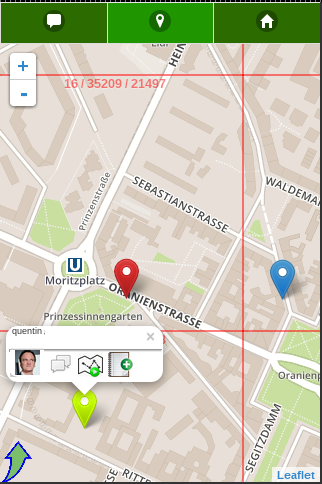
\includegraphics[scale=0.6]{bilder/screenshots/map_mobile.png} & 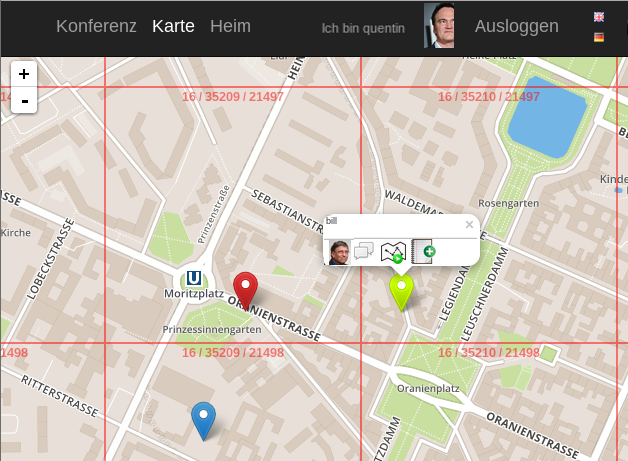
\includegraphics[scale=0.62]{bilder/screenshots/map_desktop.png} \\
	Mobiler Client & Desktop Client \\
% TODO with colspan 2. Die Kacheln sind rot umrandet und mit x/y/z-Angaben versehen
	%\multicolumn{2}{c}{}
  \end{tabulary}
  \end{adjustwidth}
  %\caption{Karten-Darstellung in VoyageX}
\end{table}

\paragraph{Marker}
Mit Markern werden feste und bewegliche Punkte auf der Karte gekennzeichnet. In VoyageX gibt es 3 Marker-Typen:
\begin{itemize}[leftmargin=*,noitemsep,topsep=1ex,parsep=0pt,partopsep=0pt]
\item 
\includegraphics[scale=0.3]{bilder/marker-icon-blue.png} \textbf{Arbeitsmarker}: Mit der Positionierung dieses Markers wird ein Punkt auf der Karte ausgewählt, den der Benutzer bearbeiten möchte. Die Positionierung kann automatisch über die GPS-Standortbestimmung, oder manuell mit einem Klick auf die Karte durchgeführt werden. Es gibt nur einen Arbeitsmarker pro Client.
\item 
\includegraphics[scale=0.3]{bilder/marker-icon-red.png} \textbf{PoI-Marker}: Kennzeichnen Points of Interest (PoI), also Orte oder Objekte. In VoyageX werden immer alle PoIs des Karten-Ausschnitts angezeigt, es wäre aber sinnvoll die Anzeige, wie bei anderen Location-Based-Apps durch Kategorie-Filter einzugrenzen (z.B. Sehenswürdigkeit, Gefahrenstelle, Gastronomie, ...)
%, welche durch eine Suchfunktion definiert werden könnten.
%Im Rahmen dieser Arbeit wurde auf dieses Feature aufgrund des dafür nötigen Aufwands verzichtet.
\item 
\includegraphics[scale=0.3]{bilder/marker-icon-yellow.png} \textbf{Peer-Marker}: Mit diesen Markern werden Positionen von den Arbeitsmarkern entfernter Benutzer (Peers) angezeigt. Voraussetzung dafür ist eine Erlaubnis des jeweiligen Peers. Die Position des Markers kann dabei durch folgende Funktions-Modi festgelegt sein:
	\begin{itemize}
		\item \textbf{Trace}: Der Marker zeigt den aktuell per GPS bestimmten Standort des entfernten Benutzers
		\item \textbf{Draw}: Der Marker zeigt die manuell festgelegte Position des entfernten Arbeistmarkers. In diesem Modus kann ein Benutzer den entfernten, ihm zugeordneten Peer-Marker mit seinem lokalen Arbeitsmarker steuern. Dabei kann er Pfade auf dem entfernten Rechner zeichnen. (siehe auch \ref{REMOTEDRAW})
	\end{itemize}
\end{itemize}

\subsubsection{Bearbeitungsfunktionen}
Das Werkzeugmenu eines Markers wird durch Mouseover oder Klicken auf den Marker geöffnet.

\paragraph{Arbeitsmarker}
Mit dem Arbeitsmarker können Funktionen und Einstellungen zur Kartenbearbeitung aufgerufen werden.

  \begin{figure}[H]
      \centering
	  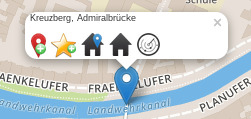
\includegraphics[scale=0.8]{bilder/screenshots/menu_arbeitsmarker.png}\\ 
  	  Werkzeugmenu des Arbeitsmarkers
  	  %\caption{Werkzeugmenu des Arbeitsmarkers}
  \end{figure}

\begin{itemize}[leftmargin=*,noitemsep,topsep=1ex,parsep=0pt,partopsep=0pt]
\item 
\includegraphics[scale=0.55]{bilder/icons/add-marker.png} \textbf{PoI eintragen}: Öffnet das Eingabeformular für PoIs an der aktuellen Marker-Position. Neben einer obligatorischen textuellen Beschreibung des PoIs muss der Typ des Anhangs ausgewählt werden. 4 Typen stehen zur Auswahl:
	\begin{itemize}[leftmargin=*,noitemsep,topsep=1ex,parsep=0pt,partopsep=0pt]
		\item \textbf{Plain Text}: Ein Plain-Text Eintrag hat keinen Anhang. Allerdings wird als Default Icon ein weisses Rauschen angezeigt. Dies motiviert den Benutzer dann vielleicht doch noch einen anschaulicheren Anhang zu wählen.
		\item \textbf{Foto}: Falls verfügbar, kann mit der Kamera des Endgeräts ein Foto aufgenommen und angehängt werden. Bei mehreren Kameras kann der Benutzer eine Auswahl treffen.
		\item \textbf{Datei}: Vom lokalen Datei-System kann eine Bild-, Audio- oder Video-Datei hochgeladen werden.
		\item \textbf{Embed}: Embeds sind Html-Code-Schnipsel mit denen Anhänge von externen Social-Media-Seiten wie Youtube oder Soundcloud eingebunden werden können. Einfache URLs werden als Link zu einer Bild-Datei interpretiert.
	\end{itemize}
\item 
\includegraphics[scale=0.15]{bilder/icons/add-bookmark.png} \textbf{Lesezeichen}: Öffnet ein Textfeld für eine Notiz zur aktuellen Markerposition. Diese Daten sind nur für den persönlichen Gebrauch des Benutzers bestimmt, und werden nicht geteilt. Bookmarks unterstützen den Benutzer beim Navigieren, Planen und Ideen sammeln.
Sie werden im Kontext-Navigations-Fenster angezeigt.
\item 
\includegraphics[scale=0.15]{bilder/icons/set-home.png} \textbf{Homebase markieren}: Markiert den aktuell ausgewählten Punkt um später schnell zu diesem "`zurückkehren"' zu können.
\item 
\includegraphics[scale=0.15]{bilder/icons/home.png} \textbf{Homebase anzeigen}: Homebase auf der Karte anzeigen.
\item 
\includegraphics[scale=0.15]{bilder/icons/radar.png} \textbf{Radar}: Öffnet eine Ansicht mit Einstellungs-Kontroll-Elementen zum Kartenkontext.
\end{itemize}

\begin{table}[H]
  %\begin{adjustwidth}{-2cm}{2cm}
  \begin{tabulary}{\columnwidth}{ C C C }
	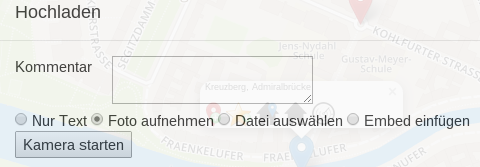
\includegraphics[scale=0.5]{bilder/screenshots/menu_arbeitsmarker_upload.png} &
	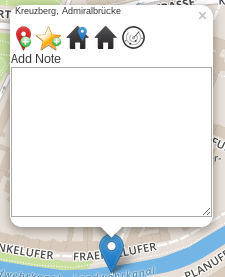
\includegraphics[scale=0.55]{bilder/screenshots/menu_arbeitsmarker_bookmark.png} &
	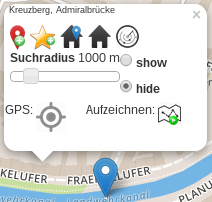
\includegraphics[scale=0.55]{bilder/screenshots/menu_arbeitsmarker_radar.png} \\
	
\includegraphics[scale=0.55]{bilder/icons/add-marker.png} &
	
\includegraphics[scale=0.15]{bilder/icons/add-bookmark.png} &
	
\includegraphics[scale=0.15]{bilder/icons/radar.png} \\
	\multicolumn{3}{c}{Weitere Schaltflächen: PoI-Eintrag, Lesezeichen, Standort-Einstellungen}
  \end{tabulary}
  %\end{adjustwidth}
  %\caption{Weitere Schaltflächen}
\end{table}

\enlargethispage{2\baselineskip} % allow 3 more lines on current page
\paragraph{PoI-Marker}
Mit dem PoI-Marker können Funktionen und Einstellungen zur PoI-Bearbeitung aufgerufen werden.

  \begin{figure}[H]
      \centering
	  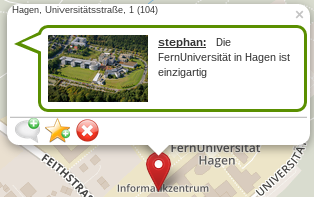
\includegraphics[scale=0.8]{bilder/screenshots/menu_poimarker.png}\\ 
  	  Anzeige eines Eintrags und Werkzeug-Menu im Popup eines Poi-Markers
  	  %\caption{Anzeige eines Eintrags und Werkzeug-Menu im Popup eines Poi-Markers}
  \end{figure}

\begin{itemize}[leftmargin=*,noitemsep,topsep=1ex,parsep=0pt,partopsep=0pt]
\item 
\includegraphics[scale=0.15]{bilder/icons/add-comment.png} \textbf{Kommentieren}: Öffnet wie 
\includegraphics[scale=0.55]{bilder/icons/add-marker.png} ein Formular zur Eingabe weiterer Beschreibungen und Media-Anhänge für den ausgewählten PoI. 
\item 
\includegraphics[scale=0.15]{bilder/icons/add-bookmark.png} \textbf{Lesezeichen}: Gleiche Funktion wie beim Arbeitsmarker.  
\item 
\includegraphics[scale=0.07]{bilder/icons/edit-note.png} \textbf{Notiz}: Lesezeichen auf PoIs sind nur für den lokalen Benutzer sichtbar und werden im Kontext-Navigations-Fenster angezeigt.
\end{itemize}

%%%%%%%%%%%%%%%%%%%%%%%%%%%%%%%%%%%%%%%%%%%%%%%%%%%%%%%%%%%%%%
% Offline Funktionalität
%%%%%%%%%%%%%%%%%%%%%%%%%%%%%%%%%%%%%%%%%%%%%%%%%%%%%%%%%%%%%%
\subsection{Offline Funktionalität}\label{5_OFFL}
%Die Anforderung zum Erhalt der Funktionsfähigkeit bei fehlender Netzwerkverbindung erfordert Lösungen für folgende Problembereiche:
Im folgenden wird gezeigt, wie mit VoyageX eine Netzwerk-Verbindungs-unabhängige Web-Anwendung realisiert wird.
%Dabei wird zunächst die allgemeine 

%Damit VoyageX auch bei fehlender Netzwerk-Verbindung genutzt werden kann, muß zunächst einmal die Ausführbarkeit der Web-Anwendung im Offline-Modus gewährleistet werden. Zusätzlich müssen in diesem Zusammenhang folgende Probleme behandelt werden:
%\begin{itemize}
%	\item Vorladen von Karten-Kachel-Bildern
%	\item Lokales speichern der Poi- und Kommunikationsdaten-Daten
%\end{itemize}
%\vspace{1ex}\noindent
%Darüber hinaus sind noch weitere Lösungen gefordert, die sich aus dem kooperativen Aspekt von VoyageX, also der erforderlichen Synchronisation der Systemdaten, ergeben. Zu diesen Lösungen gehören:
%\begin{itemize}
%	\item Erstellen von IDs zur systemweit eindeutigen Identifikation lokal erzeugter Objekte
%	\item Nebenläufigkeitsprobleme bei der Datensynchronisation
%	\item Versionierung des Systemzustandes zur Synchronisation replizierter Daten
%\end{itemize}



\subsubsection{Ausführbarkeit der Anwendung im Offline-Modus}
\paragraph{Application-Cache$^{\textbf{\ref{APPCACHE}}}$}
\addtocounter{footnote}{1}%
\footnotetext{\label{APPCACHE}\href{http://www.html5rocks.com/de/tutorials/appcache/beginner/}{Application-Cache - http://www.html5rocks.com/de/tutorials/appcache/beginner/}; letzter Zugriff: 26.04.2015}
Webseiten-Inhalte und Webanwendungs-Komponenten werden von einem Browser zwar intern zwischengespeichert, allerdings hat eine Javascript-Client-Anwendung keine absolute Kontrolle über die Cache-Strategie, und so können die Daten jederzeit verloren gehen. Um einen persistenten Zugriff auf die von einer Webseite geladenen Resourcen zu gewährleisten, wird die in Html5 standardisierte \texttt{Application-Cache}-Schnittstelle genutzt. Dazu wird im \texttt{Html-Tag} des Quellcodes über das Attribut \texttt{manifest} eine Datei referenziert, in der alle für die Client-Anwendung benötigten Resourcen (Assets) gelistet sind.
\lstset{language=Html}
\begin{lstlisting}[frame=single,numbers=none,xleftmargin=0pt]
<html manifest="voyagex.mf">
\end{lstlisting}%
Der Browser speichert diese dann dauerhaft, so daß sie, unabhängig von Netzwerkverbindung oder zwischenzeitlichen Browser-Neustarts, in der Anwendung verfügbar sind.\\
\paragraph{Templates}
Um dynamische Inhalte, wie etwa neue PoI-Einträge, im Offline-Modus darzustellen, müssen die entsprechenden Ansichten, wie in Abschnitt \ref{5_SPI} beschrieben, client-seitig aus Templates generiert werden.\\
%In VoyageX wird aufgrund der Einfacheit kein Template-Framework 
Dazu werden die Templates in die Hauptseite unsichtbar eingebunden und von der Coffee-Klasse  \texttt{VoyageX.TemplateHelper} für die Erzeugung der Ansichten verwendet.\\ \\
Ein PoI-Popup:
\lstset{language=Javascript}
\begin{lstlisting}[frame=single,numbers=none,xleftmargin=0pt]
@openPOINotePopup: (poi, marker) ->
  popupHtml = TemplateHelper.poiNotePopupHtml(poi)
  marker.getPopup().setContent(popupHtml)
  marker.openPopup()
\end{lstlisting}%
wird aus einem Template:
\lstset{language=Html}
\begin{lstlisting}[frame=single,numbers=none,xleftmargin=0pt]
<div id="tmpl_poi_notes_container" style="display: none;">
  <div tmpl-id="poi_notes_container" data-poiId="{poi_id}">
    {poi_notes}
  </div>
</div>
\end{lstlisting}%
in \texttt{VoyageX.TemplateHelper} dynamisch generiert:
\lstset{language=Javascript}
\begin{lstlisting}[frame=single,numbers=none,xleftmargin=0pt]
@poiNotePopupHtml: (poi) ->
  poiNotesHtml = ""
  for poiNote, i in poi.notes
    poiNotesHtml += poiNotePopupEntryHtml(poiNote, i)
  popupHtml = getTemplate("tmpl_poi_notes_container").
              replace(/\{poi_id\}/g, poi.id).
              replace(/\{poi_notes\}/, poiNotesHtml)
\end{lstlisting}%


\subsubsection{Vorladen der Karten-Kachel-Bilder}
Für die Kartenbearbeitung auch ohne Internet-Verbindung müssen die Karten-Kachel-Bilder
lokal vorgehalten werden.
%Dabei ist die Begrenzung des verfügbaren Speicherplatzes zu berücksichtigen.

\paragraph{Offline Zoom-Level}
Wegen der begrenzten Speicher-Kapazität werden nur Kachel-Bilder für bestimmte Zoom-Level lokal gespeichert.
Im Offline-Modus kann die Karte dann auch nur in diesen Auflösungen angezeigt werden. Die Einschränkung der Zoom-Level wird  in VoyageX mit dem LeafletJS-Plugin LimitZoom$^{\textbf{\ref{LEAFPLLZ}}}$
\addtocounter{footnote}{1}%
\footnotetext{\label{LEAFPLLZ}\href{https://github.com/Zverik/Leaflet.LimitZoom}{LimitZoom - https://github.com/Zverik/Leaflet.LimitZoom} von \href{https://github.com/Zverik}{Ilya Zverev}; letzter Zugriff: 26.02.2015} implementiert.  
%\lstset{language=Javascript}
%\begin{lstlisting}[frame=single,numbers=none,xleftmargin=0pt]
%setOnline: () ->
%  ...
%  LimitZoom._zooms.splice(0, LimitZoom._zooms.length)
%  for n in [MAP_CONTROL._minZoom..MAP_CONTROL._maxZoom]
%  	LimitZoom._zooms.push n
%
%setOffline: () ->
%  ...
%  LimitZoom._zooms.splice(0, LimitZoom._zooms.length)
%  for n in MAP_CONTROL._offlineZooms
%    LimitZoom._zooms.push n
%\end{lstlisting}%
\paragraph{Anzeige lokal gespeicherter Kacheln im Map-Viewer}
Das LeafletJS-Plugin \texttt{functionaltilelayer}$^{\textbf{\ref{LEAFPLFTL}}}$
\addtocounter{footnote}{1}%
\footnotetext{\label{LEAFPLFTL}\href{https://github.com/ismyrnow/Leaflet.functionaltilelayer}{functionaltilelayer - https://github.com/ismyrnow/Leaflet.functionaltilelayer} von \href{https://github.com/ismyrnow}{Ishmael Smyrnow}; letzter Zugriff: 26.02.2015}%
bietet die Möglichkeit, Karten-Kachel-Bilder aus dem lokalen Cache zu laden.\\
Dazu wird bei der Initialisierung der Karte für die Darstellung der Tiles-Ebene eine Instanz des \texttt{Leaflet.functionaltilelayer} an den LeafletJS-Map-Viewer übergeben (Listing \ref{lst:CL_MapInit}).
Leaflet ruft für jede zu ladende Kachel-Bild-Url eine Funktion auf, welche diese Url aus einem Template (Listing \ref{lst:CL_TSPUTempl}) generiert und zurückgibt. An dieser Stelle fängt das Tile-Layer-Plugin den Aufruf ab und leitet
ihn an die Funktion weiter, deren Referenz dem Plugin selbst bei der Initialisierung übergeben wurde - für VoyageX also die Methode \texttt{drawTile} der Coffee-Klasse \texttt{VoyageX.MapControl}:
\lstset{language=CoffeeScript}
\begin{lstlisting}[frame=single,xleftmargin=0pt]
@drawTile: (view) ->
  getStoredTileUrl(view) || noStoredTileUrl(view)

@noStoredTileUrl: (view) ->
  if APP.isOnline()
  	tileUrl = VoyageX.TILE_URL_TEMPLATE
              .replace('{z}', view.zoom)
              .replace('{y}', view.tile.row)
              .replace('{x}', view.tile.column)
              .replace('{s}', view.subdomain)
    return _getOriginalTileUrl view
  else
    return _notInCacheImage view
\end{lstlisting}%
%Die Interceptor-Methode wird für jede Kachel aufgerufen.\\
\begin{table}[H]
  \begin{tabulary}{\columnwidth}{>{\raggedleft}m{.5cm} L}
  \hline
1: & Als Parameter wird der Interceptor-Methode eine Datenstruktur übergeben aus welcher die x-,y- und z-Werte der zu ladenden Kachel gelesen werden können. \\ \hline
2: & Wenn das Kachel-Bild noch nicht lokal gespeichert wurde, wird die Methode \texttt{noStoredTileUrl} aufgerufen um die Url für das Kachel-Bild zu berechnen. \\ \hline
11: & Wenn der Client online ist wird das Kachel-Bild under der Standard-Url geladen. \\ \hline
13: & Falls keine Netzwerkverbindung besteht wird ein Platzhalter-Kachel-Bild generiert, das den Benutzer auf das Fehlen der Kachel im Cache anzeigt. \\ \hline
  \end{tabulary}
\end{table}
\enlargethispage{2\baselineskip} % allow 2 more lines on current page
%Falls keine Netzwerk-Verbindung verfügbar ist werden für nicht lokal gespeicherte Kachel-Bilder entsprechende
%Hinweise angezeigt.
%  \begin{figure}[H]
%      \centering
%	  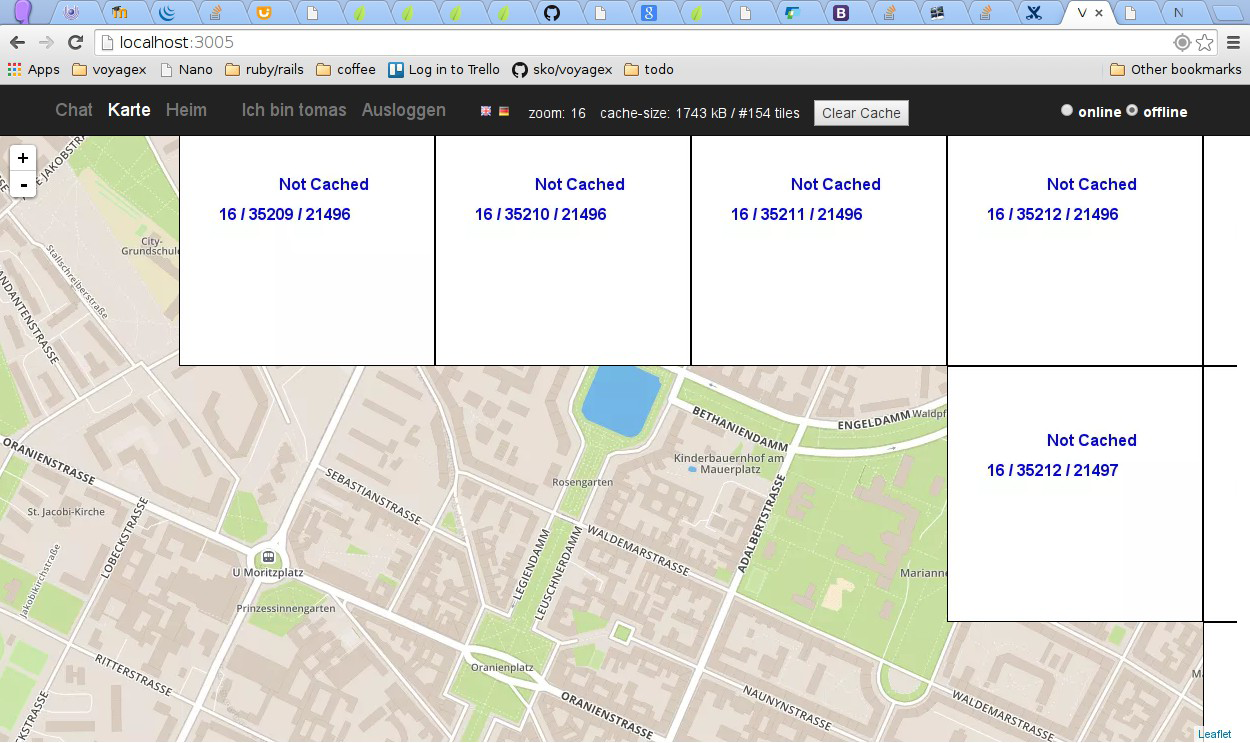
\includegraphics[scale=0.4]{bilder/map_offline.png}\\ 
%  	  \caption{Anzeige gespeicherter und fehlender Kacheln im Offline-Modus}
%  \end{figure}

\paragraph{Multithreaded File-Access: Promises$^{\textbf{\ref{CMTPROMISE}}}$}
\addtocounter{footnote}{1}%
\footnotetext{\label{CMTPROMISE}\href{http://www.html5rocks.com/en/tutorials/es6/promises/}{JS Promises - http://www.html5rocks.com/en/tutorials/es6/promises/}; letzter Zugriff: 26.02.2015}
%Der Map-Viewer generiert die Urls für die benötigten Kacheln, er kann aber nicht feststellen ob unter der Url tatsächlich eine Bild-Datei geladen werden kann. Wenn die Netzwerk-Verbindung abbricht während der Map-Viewer die Kachel-Bild-Urls bereits generiert und in den HTML-Dom-Baum eingebunden hat, dann werden die
Der Map-Viewer erwaret also beim Aufruf von \texttt{drawTile} eine Kachel-Url als Rückgabewert. Nun muß folgendes Problem für das Laden lokal gespeicherter Kachel-Bilder gelöst werden: Während Zugriffe auf localStorage synchron erfolgen können, bietet die File-API aber keine Möglichkeit zum synchronen Lesen oder Speichern von Dateien$^{\textbf{\ref{CMTASYNCIDB}}}$%
\addtocounter{footnote}{1}%
\footnotetext{\label{CMTASYNCIDB}An dieser Stelle sei noch angemerkt daß auch eine Client-seitige Persistenz-Implementierung mit IndexedDB in einem Multithreaded Kontext abläuft}. Deshalb gibt \texttt{drawTile} keine URLs, sondern Javascript-\texttt{Promises} zurück$^{\textbf{\ref{CMTPROMFORLEAF}}}$%
\addtocounter{footnote}{1}%
\footnotetext{\label{CMTPROMFORLEAF}Die Möglichkeit zur Promise-Verarbeitung ist im functionaltilelayer-Plugin bereits explizit implementiert}
%Damit die im Map-Viewer lokal gespeicherte Kachel-Bilder anzeigen kann gibt es 2 Möglichkeiten:
%\begin{itemize}
%\item Er lädt sie von Urls aus dem Netz und die Anwendung überschreibt 
%\item \textbf{Karte}: In dieser Ansicht werden die Karte sowie Navigations- und Steuerungs-Elemente angezeigt.
%\item \textbf{Heim}: In der Heimansicht befinden sich die Eingabe- und Steuerungs-Elemente zur Verwaltung der Benutzer- und Kontakt-Daten.
%\end{itemize}
%Der Map-Viewer soll im Offline-Modus lokal gespeicherte Kachel-Bilder anzeigen, 
%Für das Laden eines Bildes wird in Javascript ein neuer Thread gestartet. Allerdings erwartet 
%Damit der Map-Viewer auf die Bild-Daten dennoch wartet, erhält er eine Javascript-Promise.
%Um ein lokal gespeichertes Kachel-Bild anzuzeigen, muß der Map-Viewer auf die 
Im folgenden Code-Snippet wird gezeigt, wie eine Promise nach dem asynchronen Lesen einer über die File-API
aufgelöst (resolved) wird:
\lstset{language=CoffeeScript}
\begin{lstlisting}[frame=single,xleftmargin=0pt]
getTile: (xYZ) ->
  deferred = $.Deferred()
  _getTileFile xYZ, deferred
  return deferred.promise  

_getTileFile: (xYZ, deferred) ->
  path = '/'+xYZ[2]+'/'+xYZ[0]+'/'+xYZ[1]
  getDirectory(path).getFile(path, {}, (fileEntry) ->
  	  deferred.resolve fileEntry.toURL TILE_IMAGE_CONTENT_TYPE
  	, (error) ->
  	  deferred.resolve MapControl.noStoredTileUrl(_xYZToView(xYZ))
\end{lstlisting}
\begin{table}[H]
  \begin{tabulary}{\columnwidth}{>{\raggedleft}m{.5cm} L}
  \hline
2: & Für das asynchrone Lesen der Kachel-Bild-Datei wird ein \texttt{Deferred} Objekt erzeugt, welches Callback-Methoden einer \texttt{Promise} verwaltet \\ \hline
4: & Die \texttt{Promise} wird anstatt einer echten Url zurückgegeben  \\ \hline
9: & Die Deferred-Callback-Methoden \texttt{resolve} werden aufgerufen, nachdem die Bild-Datei vollständig gelesen und dem Deferred-Objekt in Form einer Filesystem-Url über den resolve-Aufrufe übergeben wurde.\\ \hline
11: & Im Fehlerfall, wenn die Datei nicht existiert, wird die Promise nach einer Original-Kachel-Bild-URL oder einer Info-Bild-URL aufgelöst \\ \hline
  \end{tabulary}
\end{table}
%Im folgenden Code-Snippet wird gezeigt, wie die Bilddaten von einer Url geladen und lokal gespeichert werden.
%\lstset{language=CoffeeScript}
%\begin{lstlisting}[frame=single,xleftmargin=0pt]
%loadReadyImage: (imgUrl, xYZ) ->
%  deferred = $.Deferred()
%  img = new Image
%  img.onload = (event) ->
%    base64ImgDataUrl = _toBase64 $('#tile_canvas')[0], this
%    storeImage xYZ, base64ImgDataUrl
%    deferred.resolve base64ImgDataUrl
%  img.src = imgUrl
%  return deferred.promise  
%\end{lstlisting}%
%\begin{table}[H]
%  \begin{tabulary}{\columnwidth}{>{\raggedleft}m{.5cm} L}
%  \hline
%2: & Für das Laden des Bildes ein \texttt{deferred} Objekt erzeugt welches callback-Aufrufe einer \texttt{Promise} verwaltet \\ \hline
%4: & Die Callback-Methode wird aufgerufen wenn die Bild-Datei vollständig geladen wurde. Die Bild-Daten werden dann auf einem Canvas-Objekt in eine base64-Data-Url konvertiert, die lokal gespeichert wird. Mit dieser Url wird dann die \texttt{Promise} eingelöst, also der Map-Viewer wird benachrichtigt daß er das Bild jetzt unter dieser (lokalen) Url laden soll.\\ \hline
%9: & Die \texttt{Promise} wird anstatt einer echten Url zurückgegeben  \\ \hline
%  \end{tabulary}
%\end{table}
\enlargethispage{3\baselineskip} % allow 3 more lines on current page
Im Map-Viewer wird unterdessen wie folgt auf die Bild-Url gewartet:
\lstset{language=CoffeeScript}
\begin{lstlisting}[frame=single,numbers=none,xleftmargin=0pt]
promise = drawTile {tile: {column: 13456, row: 546}, zoom: 16}
promise.then (url) ->
  renderImage url
\end{lstlisting}
\vspace{2ex}
Im folgenden ist die Sequenz beim Laden eines Kachel-Bildes in VoyageX noch einmal vollständig dargestellt. %Im synchronen Aufruf von \texttt{deferred} wird eine \texttt{Promise} zurückgegeben. Diese wird dann asynchron mit einer Data-Url einer bereits lokal gespeicherten oder einer erst zu ladenden und anschließend zu speichernden Datei aufgelöst.
%  webp - data-url
%functional-til-layer unterstützt aber javascript-promises, eine promis implementierz u.a. den calback then
%der aufgerufen wird sobald ein wert verfügbar ist.
%mit promises werden auch javascript new Image geladen.
%nahcdem de aufrufe nicht syncron hintereinander ausgeführt.
%wirk das seh komplex und man muss 
%und jetzt das sequenzdiagramm
%\enlargethispage{2\baselineskip} % allow 2 more lines on current page
  \begin{figure}[H]
      \centering
	  \includegraphics[scale=0.7]{bilder/uml/loadTile.png}\\ 
  	  \caption{Ladevorgang - synchroner Aufruf von \texttt{getTile} und asynchrones Lesen einer Datei mit Auflösung der Promise}
  \end{figure}
%  \begin{figure}[H]
%      \centering
%	  \includegraphics[scale=0.7]{bilder/uml/saveTile.png}\\ 
%  	  \caption{Ladevorgang 2 - asynchrones Schreiben einer Datei mit Auflösung der Promise}
%  \end{figure}

\paragraph{Vorladestrategien}
Beim Vorladen der Kachel-Bilder werden für den dargestellten Kartenausschnitt auch die Kachel-Bilder der darüberliegenden offline-Zoom-Level vorgeladen, damit ein Benutzer ausgehend von der niedrigsten Auflösung
den im offline-Modus verfügbaren Bereich auf der Karte finden kann.
\enlargethispage{2\baselineskip} % allow 3 more lines on current page
	\begin{table}[H]
  		\begin{adjustwidth}{-0.3cm}{0.3cm}
		\centering
		\begin{tabulary}{\columnwidth}{C >{\centering}m{1cm} C >{\centering}m{1cm} C}
			\includegraphics[scale=0.5]{bilder/screenshots/offline_16.png} & & \includegraphics[scale=0.5]{bilder/screenshots/offline_12.png} & & \includegraphics[scale=0.5]{bilder/screenshots/offline_4.png} \\
		\end{tabulary}
  		\end{adjustwidth}
	\end{table}
Für das Vorladen werden in VoyageX 3 verschiedene Strategien implementiert:
\begin{itemize}[leftmargin=*,noitemsep,topsep=1ex,parsep=0pt,partopsep=0pt]
	\item \textbf{Umkreis um den aktuellen Standort}: Bei dieser Strategie werden nach jeder Kartenverschiebung durch den Benutzer die Kacheln in einem einstellbaren Radius um den aktuellen Standort vorgeladen. Dabei werden wahrscheinlich auch viele unbenötigte Kacheln geladen - insbesondere wenn sich der Benutzer länger in eine bestimmte Richtung bewegt, und der Radius groß gewählt wurde.
	\item \textbf{Bewegungsrichtung}: Folgender sehr einfache Vorlade-Algorithmus, der die Bewegungsrichtung und die Geschwindigkeit berücksichtigt, wird von VoyageX implementiert:
	\begin{itemize}[leftmargin=*,noitemsep,topsep=1ex,parsep=0pt,partopsep=0pt]
%		\item
%		Die Grundidee ist folgende: Die Ungenauigkeit einer Messung der Bewegungsrichtung kann mit der Höhe der Geschwindigkeit wachsen.\\
%		Dazu folgende Algorithmus-Ausgangsfrage: Wenn der letzte, vor einer Stunde gemerkte Standort des Benutzers 100km in südlicher Richtung - vom aktuellen Standort betrachtet - war, dann wird er eine Stunde später 100km nördlich von der aktuellen Position sein. Falls der Benutzer allerdings vor 5 Minuten sein Ziel erreicht hat ist die Vorhersage sehr ungenau.\\
%		Die Idee für einen Algorithmus ist es jetzt, im Vorhersage-Algorithmus die Zeit-Abhängigkeit durch eine Entfernungs-Abhängigkeit ersetze - also nicht mehr wie im Beispiel jede Stunde zu messen, sondern ungefähr alle 100 Meter, wobei diese nicht exakt eingehalten werden müssen sondern, wie im folgenden ersichtlich wird, nur als Berechnungsgrundlage dienen.
%		\item Mit dem 100 Meter Richtwert wird zunächst jenes Zeit-Interval berechnet, in dem der Benutzer 100 Meter zurücklegt. Der Unterschied ist daß ich statt mit einem Wert "`100m / Zeiteinheit"` mit einem Wert
%		"`10min / Entfernungseinheit"` rechne. Da hat zur folge daß bei Steigender Geschwindigkeit öfters gemessen wird und die maximale Fehler-DIstanz die gewählte Entfernungseinheit ist.
%		\item Nach jeder Standort-Verschiebung wird also die nächste Position dann einfach als Verlängerung der Geraden (Luftlinie) von der zuletzt gemerkten Position über aktuelle Position um die gleiche Distanz berechnet. bei einer geschwindigkeit von 100 km/h wird  alle 0,001 stunden (3,6) sekunden  gemessen/veglichen.
%		bei 5 kmh also 0,08 stundrn alos alle 72 sekunden
		% bei 100kmg ich vergleiche also den standpunkt mit dem vor 3,6 sekunden
%		Die Kacheln werden dann entsprechend dem Radius in der richtung vorgeladen.
		\item Alle 100 Meter wird die Bewegungsrichtung bestimmt.
		\item Die Kacheln werden 1000 Meter in der Bewegungsrichtung vorgeladen. Dazu wandert der Algorithmus wiederholt horizontal bis zum Kachelende und dann vertikal bis zur Verbindungsgeraden zwischen Ausgangsort und vorhergesagter Position. Die gesuchten Kacheln sind all jene, deren Kanten$^{\textbf{\ref{CMTPATHALGO1}}}$
\addtocounter{footnote}{1}%
\footnotetext{\label{CMTPATHALGO1}1 bei Endkacheln , 2 bei Mittelkacheln} von der Verbindungsgeraden horizontal oder vertikal geschnitten werden, oder nur 1 Kachel falls Ausgangs- und Zielpunkt nah genug beieinander liegen.\\
Abbildung \ref{fig:PATH_PRED} illustriert die Vorgehensweise: Der blaue Marker zeigt die aktuelle Position. Dir kurze grüne Linie nach links-oben zeigt die 100-Meter-Strecke zur vorigen Position. Die gelbe Verlängerung der Linie über die aktuelle Position hinaus führt zur 1000 Meter entfernten vorhergesagten Position, welche mit einem "`Beam"'-Marker (\includegraphics[scale=0.4]{bilder/icons/marker-icon-beam.png}) gekennzeichnet ist. Die treppenförmige blaue Linie folgt dem Kachel-Auswahl-Algorithmus.
  \begin{figure}[H]
  	\begin{adjustwidth}{-1cm}{1cm}
      \centering
	  \includegraphics[scale=0.6]{bilder/screenshots/move_prediction.png}\\ \vspace{0.8cm}
  	  \caption{Veranschaulichung des Kachel-Auswahl-Algorithmus mittels Pfad-Vorhersage}
  	  \label{fig:PATH_PRED}
  	\end{adjustwidth}
  \end{figure}
		
	\end{itemize}
	\item \textbf{Manuelle Auswahl}: Karten-Kacheln auf denen sich gespeicherte Locations (Bookmarks) befinden, werden ebenfalls lokal gespeichert.
\end{itemize}

%\subsubsection{Lokales Speichern von PoI-Daten und Push}
\subsubsection{PoI-Daten}
\paragraph{IDs}
In klassischen Webanwendungen werden Objekte erzeugt, indem die Werte der Objekt-Eigenschaften vom Client an den Server geposted, um dort zu einem Objekt gekapselt und mit einer ID persistiert zu werden. Der Client erhält die ID des Objekts dann erst mit Antwort des Servers. Da in VoyageX ein Benutzer Objekte auch ohne Server-Verbindung erzeugen kann, muß schon clientseitig eine ID generiert werden.\\
Damit diese ID nun auch systemweit eindeutig
ist gibt es für deren Erzeugung mehrere Möglichkeiten, beispielsweise könnten \texttt{Universally Unique Identifiers (UUIDs)}$^{\textbf{\ref{CMTUUID}}}$
\addtocounter{footnote}{1}%
\footnotetext{\label{CMTUUID}\href{http://de.wikipedia.org/wiki/Universally\_Unique\_Identifier}{UUID - http://de.wikipedia.org/wiki/Universally\_Unique\_Identifier}; letzter Zugriff: 06.05.2015} verwendet werden, oder es könnte ein lokal erzeugtes PoI-Objekt mit einem SHA-1 Hash aus Benutzer-ID, Geo-Koordinaten und lokalem Timestamp systemweit eindeutig identifiziert werden. Allerdings hat die client-seitige Erstellung von IDs auch Nachteile:
\begin{itemize}[leftmargin=*,noitemsep,topsep=1ex,parsep=0pt,partopsep=0pt]
\item Es entsteht dadurch eine Abhängigkeit des Systems von der gewählten Generierungs-Methode, da sie auf allen Clients gleich sein muss.
\item Ohne server-seitige Kontroll-Anwendungs-Logik könnte eine Daten-Inkonsistenz durch bösartig manipulierte IDs hervorgerufen werden.$^{\textbf{\ref{CMTINCONS}}}$
\addtocounter{footnote}{1}%
\footnotetext{\label{CMTINCONS}Ein Client könnte versuchen, mit einer einzigen ID mehrere Objekte anzulegen}
%\item Nachdem jeder PoI nur einmal erzeugt werden soll muss für den Kollisionsfall Anwendungs-Logik entworfen werden welche die ID dann bei mindestens einem Benutzer korrigieren muss.
%\item Für den gutartigen ID-Kollisionsfall müsste zusätzlich client-seitige Anwendungs-Logik entworfen werden welche die ID dann bei mindestens einem Benutzer korrigieren muss.
\item Um Kollisionen zu vermeiden sind clientseitige IDs in der Regel mit 128 Bit relativ groß, also möglicherweise viel größer als nötig.
\end{itemize}
Für VoyageX wird daher eine Lösung implementiert, bei der systemweite IDs Server-seitig generiert werden.
\paragraph{Daten-Synchronisation}
%Für VoyageX wird nun eine für die prototypische Implementierung ausreichende und sehr einfache Lösung gewählt, und damit folgender Ablauf implementiert:
Folgende Schritte werden von VoyageX für das Speichern von PoI-Daten implementiert: 
\begin{enumerate}[leftmargin=*,noitemsep,topsep=1ex,parsep=0pt,partopsep=0pt]
\item Das Objekt wird mit einer temporären lokalen ID gespeichert, in eine Upload-Queue geschrieben und in der Benutzeroberfläche angezeigt.
\item Wenn oder sobald eine Verbindung zum Backend besteht werden alle in der Upload-Queue gespeicherten Objekte hochgeladen.
%Allerdings wird davor noch einmal die aktuelle Master-Commit-ID vom Backend abgefragt und gegebenenfalls die lokale Kopie aktualisiert.
\item 
\begin{enumerate}[label=\alph*),leftmargin=*,noitemsep,topsep=1ex,parsep=0pt,partopsep=0pt]
\item Im Backend werden die Objekte mit einer endgültigen systemweiten ID gespeichert, die dann
%zusammen mit der temporären 
an den Client des Autors zurückgeschickt wird
\item Alle anderen (online-)Clients werden mit einer Pull-Request-Nachricht aufgefordert ihre Daten zu 		aktualisieren.
\end{enumerate}
\item
\begin{enumerate}[label=\alph*),leftmargin=*,noitemsep,topsep=1ex,parsep=0pt,partopsep=0pt]
\item Im Client des Autors werden alle Elemente aus der Upload-Queue entfernt und mit der ID vom Backend aktualisiert
\item Die anderen (online-)Clients holen sich ggf. das Änderungs-Log vom Backend, aktualisieren lokale Daten und Ansicht und informieren den lokalen Benutzer.
\end{enumerate}
\end{enumerate}
%Wenn ein Benutzer den "`Sichern"'-Button im PoI-Eingabeformular klickt werden die Daten zunächst lokal %gespeichert.
%\lstset{language=CoffeeScript}
%\begin{lstlisting}[frame=single,numbers=none,caption={Methode send der Coffee-Klasse Comm},captionpos=b]
%	$(document).on 'click', '#upload_button', (event) ->
%\end{lstlisting}
%\enlargethispage{4\baselineskip} % allow 3 more lines on current page
Das Speichern von PoI-Daten im VoyageX-Client wird also in 2 Phasen durchgeführt:\\
\subparagraph{lokales Speichern (\texttt{Commit}):}
Das folgende Sequenz-Diagramm zeigt die an Schritt 1 beteiligten Coffee-Script-Klassen und aufgerufenen Funktionen im Frontend.
\enlargethispage{2\baselineskip} % allow 3 more lines on current page
  \begin{figure}[H]
  	\begin{adjustwidth}{-0.3cm}{0.3cm}
      \centering
  	  \includegraphics[scale=0.7]{bilder/uml/queuePoiNote.png}
  	  \caption{Daten-Synchronisations-Phase 1 - lokales Speichern im Frontend}
  	\end{adjustwidth}
  \end{figure}
\noindent
%Nach dem lokalen Speichern ist der neue PoI mit einer temporären ID im \texttt{localStorage} gespeichert und in die Upload-Queue eingetragen.
Die nachfolgende Abbildung zeigt einen alten PoI mit ID 30 sowie einen neuen PoI mit ID -1428573106 samt zugehöriger Upload-Warteschlange im \texttt{localStorage}.
  \begin{figure}[H]
  	\begin{adjustwidth}{-0.4cm}{0.4cm}
      \centering
  	  \includegraphics[scale=0.7]{bilder/screenshots/queue_localStrorage_1.png}
  	\end{adjustwidth}
  \end{figure}
\vspace{1ex}
%Sobald der Client online ist (ggf. sofort) wird die PoI-Note-Queue zum Backend hochgeladen:
\subparagraph{Synchronisation mit Backend (\texttt{Push}):}
Das folgende Sequenz-Diagramm zeigt die an den Schritten 2 und 4 beteiligten Coffee-Script-Klassen und aufgerufenen Funktionen im Frontend, sowie die an Schritt 3 beteiligten Ruby-Klassen im Backend. 
  \begin{figure}[H]
  	\begin{adjustwidth}{-1.5cm}{1.5cm}
      \centering
  	  \includegraphics[scale=0.7]{bilder/uml/syncPoiNoteQueue.png} \\
  	  \caption{Daten-Synchronisations-Phase 2 - Upload der Daten, Synchronisation im Backend und Notifikation über Faye}
  	\end{adjustwidth}
  \end{figure}
\noindent
%Nach dem Push wird die temporäre ID mit der Backend-generierten ID überschrieben und die PoI-Referenz aus der Upload-Queue gelöscht.
Die nachfolgende Abbildung zeigt das localStorage des Autors nachdem der neue PoI mit der ID 31 aktualisiert und die Upload-Warteschlange gelöscht wurde.
  \begin{figure}[H]
  	\begin{adjustwidth}{-0.8cm}{0.8cm}
      \centering
  	  \includegraphics[scale=0.7]{bilder/screenshots/queue_localStrorage_2.png}
  	\end{adjustwidth}
  \end{figure}
\noindent
Im Backend kann bei komplexen Operationen im Falle einer synchronen Abarbeitung (zwischen Request und Response) die Serverlast so hoch werden, daß nachfolgende Requests durch Timeouts möglicherweise blockiert werden. Deshalb wird in VoyageX die Daten-Zusammenführung asynchron in einem Resque-Job abgearbeitet.
%Am Ende dieses Jobs werden folgende System-Nachrichten
%\begin{itemize}[leftmargin=*,noitemsep,topsep=1ex,parsep=0pt,partopsep=0pt]
%\item Der "`pushende"' Client   
%\item \includegraphics[scale=0.07]{bilder/icons/edit-note.png} \textbf{Notiz}: Wie beim Lesezeichen kann man eine Notiz mit der aktuellen Marker-Position assoziieren, diese wird aber nicht in der Kontext-Navigation als Lesezeichen angezeigt. Sie bezieht sich direkt auf den PoI.
%\end{itemize}
%, und die Commit-ID des Benutzers anschließend über eine System-Callback aktualisiert.

\enlargethispage{2\baselineskip} % allow 3 more lines on current page
\paragraph{Versionierung und Nebenläufigkeit}
Synchrone kooperative Systeme erlauben es mehreren verteilten Benutzern zur gleichen Zeit an einer gemeinsamen Datenbasis zu arbeiten. Dazu werden oft auch bei online-Anwendungen Datensätze repliziert, um die Anwendungs-Performance durch den Umgehung der Netzwerk-Latenz zu steigern. Bei VoyageX erhält jeder Benutzer
eine Kopie der für ihn relevanten Systemdaten, also jener Daten, die in Bezug zu seinem aktuellen Standort bzw. zu seinem lokalen Kartenausschnitt stehen. Eine Aktualisierung der Daten wird dann durch 2 Ereignisse ausgelöst:
\begin{itemize}[leftmargin=*,noitemsep,topsep=1ex,parsep=0pt,partopsep=0pt]
\item Der Client des Benutzers wird im online-Modus per System-Calls über Aktualisierungen durch andere Benutzer informiert
\item  Der Client wechselt vom offline- in den online-Modus
\end{itemize}
Um festzustellen ob der Client eine Aktualisierung benötigt wird jeder System-Daten-Änderung eine Commit-ID zugeordnet.%
%- wobei eine Änderung auch mehrere Objekte umfassen kann.
Der Client kann also die aktuelle Commit-ID der Systemdaten mit seiner eigenen vergleichen, um die Notwendigkeit einer Aktualisierung festzustellen.\\ \\ 
Die Versionierung der Daten wird mit einem Git$^{\textbf{\ref{CMTGIT}}}$%
\addtocounter{footnote}{1}%
\footnotetext{\label{CMTGIT}\href{http://de.wikipedia.org/wiki/Git}{Git - http://de.wikipedia.org/wiki/Git}; letzter Zugriff: 06.05.2015}%
-Repository verwaltet. Dabei gibt es 2 Möglichkeiten, wie Client-Replikationen mit dem System-Master-Branch synchronisiert werden können:
\begin{itemize}[leftmargin=*,noitemsep,topsep=1ex,parsep=0pt,partopsep=0pt]
\item für jeden Client wird ein eigenes Repository im Backend angelegt
\item für jeden Client wird ein Branch in einem Arbeits-Repository im Backend angelegt
\end{itemize}
Die Backend-Webanwendung nutzt die Ruby-Klasse \texttt{VersionManager} um auf Git-Funktionen zuzugreifen.
Die benötigten Synchronisations-Methoden werden von VersionManager in einer API gekapselt, wie im folgenden Code-Listing beispielhaft an der Methode \texttt{merge} gezeigt wird:
\lstset{language=Ruby}
\begin{lstlisting}[frame=single,xleftmargin=0pt,numbers=none]
  def merge cur_branch
  	...
    `git #{@git_args} fetch`
    `git #{@git_args} rebase origin/#{@master}`
    set_branch @master
    `git #{@git_args} merge #{branch}`
    `git #{@git_args} push origin #{branch}`
    set_branch cur_branch
  end
\end{lstlisting}
Mit der Wahl eines Versionierungs-Systems wie Git ließe sich auch die Anzeige unterschiedlicher Daten-Ansichten einfach in die Anwendung integrieren: Für jede gewünschte Sicht könnte ein eigener Branch angelegt werden, und Benutzer könnten über Checkouts zwischen verschiedenen Sichten wechseln. Allerdings wären Sichtwechsel dann nur im Online-Modus möglich.
%Die zweite Methode ist wesentlich Resourcen-schonender und wir deshalb für VoyageX gewählt.\\
%Wenn ein Client synchronisiert wird nur ein temporäres Arbeits-Verzeichnis mit dem aktuellen Commit des Clients angelegt.
%Nache einem Push durch einen Client können per \texttt{diff} die Änderungen analysiert werden, und anschließend zusammengeführt.
%Alle online-Clients erhalten eine Systembenachrichtigung, offline-Clients werden im Rahmen ihres nächsten Synchronisations-Request benachrichtigt.
%auf diese art wird der client über änderungen informiert die ihn aber vielleicht gart nicht betreffen weil
%die änderungen ausserhalb seines kartenausschnitts sind. andererseitsmuß das auch nicht zwangsläufig ein ausschlusskriterium sein denn der benutzer könnte sich ja in naher zukunft doch auch in dem bereicht aufhalten. es gibt auch verscheidene strageien die eine sinnvolle synchronisation haben kann. es wäre auch denkbar nach interessen oder gruppen-zugehörigkiet daten auszuwählen.

\subsubsection{Kommunikations-Daten}
Sowohl P2P-Nachrichten als auch Broadcast-Nachrichten werden im Backend gespeichert, damit diese einem offline-Benutzer zugestellt werden können sobald er wieder online ist.
Bei VoyageX wird keine sequentielle Konsistenz für Chat-Nachrichten implementiert - die Reihenfolge kann daher bei in den verschiedenen Clients variieren. 
%Kommunikations-Nachrichten werden von jedem Client sequentiell gespeichert und benötigen keine IDs, da sie nicht weiter bearbeitet werden können.
%Darüber hinaus gilt für die Speicherung von Kommunikations-Daten folgendes:
%\begin{itemize}[leftmargin=*,noitemsep,topsep=1ex,parsep=0pt,partopsep=0pt]
%%\item Nachrichten können nachträglich nicht geändert werden
%\item P2P-Chat-Nachrichten werden nur lokal gespeichert. Die Sortierung kann bei verschiedenen Clients variieren.
%\item Conference-Chat-Nachrichten erhalten einen Backend-System-Timestamp wenn sie am Kommunikations-Server eintreffen und werden direkt an alle Empfänger weitergeleitet. Die Sortierung kann bei verschiedenen Clients variieren.
%\end{itemize}
 

%%%%%%%%%%%%%%%%%%%%%%%%%%%%%%%%%%%%%%%%%%%%%%%%%%%%%%%%%%%%%%
% Interaktion
%%%%%%%%%%%%%%%%%%%%%%%%%%%%%%%%%%%%%%%%%%%%%%%%%%%%%%%%%%%%%%

\subsection{Interaktion}\label{5_INTER}
Interaktion wird über den Austausch von Nachrichten realisiert. In VoyageX können nach Teilnehmer-Typus 2 Formen der Interaktion unterschieden werden:
\begin{itemize}
	\item \textbf{Benutzer (User) - System}. Beispiele für Nachrichten-Inhalte:
		\begin{itemize}
			\item Allgemeine Anwendungs-Steuerung
			\item Benachrichtigungen über neu erstellte PoI-Einträge
		\end{itemize}
	\item \textbf{Benutzer (User) - entfernter Benutzer (Peer)}. Beispiele für Nachrichten-Inhalte:
		\begin{itemize}
			\item Chat-Nachrichten (1 oder mehrere Empfänger)
			\item Standort-Angaben von Benutzern
			%\item Darstellungs-Elemente in Karten von Peers steuern (z.B. "`Pfad zeichnen"')
		\end{itemize}
\end{itemize}
Für unterschiedliche Interaktions-Funktionen werden verschiedene logische Kommunikations -Kanäle und spezifische Nachrichten-Formate definiert, die in den folgenden Abschnitten beschrieben werden.

\subsubsection{Follow-Beziehung = Kontakt}
Der Nachrichten-Austausch zwischen Benutzern erfordert eine gegenseitige Autorisierung. Jeder Benutzer muss selbst bestimmen (können), wer seine Aktionen verfolgen darf, und über wessen Aktionen er selbst informiert werden möchte. In VoyageX wird nur ein einfaches Autorisierungs-Konzept implementiert, es gibt nur einen Berechtigungs-Status, der bei VoyageX über das \texttt{Follow}-Flag gesetzt wird.
%Ein User kann nur mit jenen Peers interagieren, die ihm eine Follow-Berechtigung erteilt haben.
Die Follow-Berechtigung wird folgendermaßen erworben:
\begin{enumerate}[leftmargin=*,noitemsep,topsep=1ex,parsep=0pt,partopsep=0pt]
\item Ein User sendet einen Follow-Request an einen Peer. 
\item Der Peer wird, wenn oder sobald er online ist, akkustisch und/oder visuell auf die neue Anfrage hingewiesen und kann diese
%in seiner Administrations-Ansicht
sofort oder auch später entscheiden.
\item Der User wird, wenn oder sobald er online ist, ebenfalls akkustisch und/oder visuell über die Entscheidung des Peers informiert. 
\end{enumerate}
Eine Follow-Beziehung kann jederzeit von jedem der beiden Interaktions-Partner wieder beendet werden.

\subsubsection{Kommunikations-Kanäle}
Die Infrastruktur für die Interaktion wird mit einem \texttt{Publish-Subscribe-Messaging} System realisiert. Dabei werden für die Kommunikation logische Kanäle (Channels) definiert. Für den Empfang von Nachrichten wird ein Channel abonniert (subscribe), zum Versenden werden Nachrichten in einen Channel geschrieben (publish).\\ Für die Umsetzung der Kommunikations-Anforderungen in VoyageX müssen 2 Arten von Verbindungen bereitgestellt werden:
\newpage
\begin{itemize}[leftmargin=*,noitemsep,topsep=1ex,parsep=0pt,partopsep=0pt]
\item \textbf{Broadcast (BC):}
	\begin{itemize}
		\item %
%Jedem Benutzer ist eine BC-Verbindung zugeordnet.
Nachrichten an mehrere Empfänger werden vom VoyageX-Client eines Benutzers in einen von autorisierten Peers abonnierten Broadcast-Kanal des Benutzers geschrieben. Der Kommunikations-Server blockiert in diesem Kanal Nachrichten die von Clients anderer Benutzer gesendet werden.
		\item Das System veröffentlicht Nachrichten die alle Benutzer erhalten sollen, beispielsweise Daten-Aktualisierungs-Benachrichtigungen, in einem allgemeinen System-Kanal.
	\end{itemize}

\item \textbf{Peer-To-Peer (P2P)}: 
	\begin{itemize}
		\item %
Jedem Benutzer ist ein P2P-Kanal zugeordnet, den er als einziger abonniert und in den alle Peers private Nachrichten an den Benutzer schreiben können. Der Kommunikations-Server blockiert Abonnements dieses Kanals durch Clients anderer Benutzer.
%Für das versenden von Nachrichten an einen einzelnen Empfänger werden diese vom VoyageX-Client des Senders in einen P2P-Kanal des Empfängers geschrieben. Der Empfänger ist der einzige Abonnent eines P2P-Kanals, der Kommunikations-Server blockiert Abonnements von anderen Benutzern. Für den Empfang privater Nachrichten abonniert jeder VoyageX-Client für seinen Benutzer P2P-Kanal.
		\item Eine Sonderform eines P2P-Kanals ist der benutzergebundene System-Kanal. Für jeden Benutzer wird genau ein Systemkanal definiert, den ausschließlich der Client des Benutzers und der Server abonnieren, und in den nur diese beiden schreiben. Im Gegensatz zu den anderen P2P-Channels ist dieser Kanal bidirektional.
	\end{itemize}
\end{itemize}
In den folgenden 3 Abbildungen werden Kommunikations-Eigenschaften und Verhalten der verschiedenen Kanal-Typen veranschaulicht. Lesen von Nachrichten wird durch Pfeile vom Kanal zum Benutzer dargestellt, Schreiben mit einem Pfeil vom Benutzer zum Kanal. Die Blitze kennzeichnen nicht erlaubte Aktionen. In den Kanal-Darstellungen sind Verbindungs-Art und Kanal-Identifikation angegeben, wobei sich letztere wie folgt zusammensetzt:\\ \\
/\textit{Kanalname}[@\textit{Benutzer-ID}[\_\textit{Verbindungstyp}]]\\ \\
Zusätzlich können Nachrichten bei Bedarf verschlüsselt werden. 
	%\multicolumn{2}{C}{} \\
%\begin{table}[H]
%  \begin{tabulary}{\columnwidth}{ C  C }
%	/talk@a3ri7vxl5 & /talk@a3ri7vxl5\_p2p \\
%	\multicolumn{2}{>{\centering}m{2.65cm}}{\includegraphics[scale=0.5]{bilder/ps_infrastructure.png}} \\
%	(BC) & (P2P)
%  \end{tabulary}
%  \caption{Beispiele für die beiden Kanäle eines Benutzers}
%\end{table}
%\enlargethispage{3\baselineskip} % allow 3 more lines on current page
  \begin{figure}[H]
      \centering
	  \includegraphics[scale=0.47]{bilder/ps_infrastructure.png}
  	  \caption{Ein BC- und ein P2P-Kanal eines Benutzers}
  	  \label{fig:BCANDP2PCHANNEL}
  \end{figure}
  \begin{figure}[H]
      \centering
	  \includegraphics[scale=0.47]{bilder/ps_infrastructure_sys_bc.png} 
  	  \caption{Der allgemeine System-Kanal (Sys-BC)}
  \end{figure}
  \begin{figure}[H]
      \centering
	  \includegraphics[scale=0.47]{bilder/ps_infrastructure_2.png}
  	  \caption{Der System-Kanal eines Benutzers (Sys-P2P)}
  \end{figure}
\noindent
Mit diesen Kanal-Typen werden nun folgende logischen Kanäle und die darüber ausgetauschten Nachrichten-Formate definiert:
%Im folgenden werden die logischen Kanäle und die darüber implementierten Funktionen beschrieben. Nachrichten werden im JSON-Format ausgetauscht.% und kapseln dabei die Funktions-Parameter.
%Alle Nachrichten werden als JSON-Objekte transportiert. Für die verschiedenen Interaktions-Formen werden folgende logischen Channels mit spezifischen Nachrichten-Formaten definiert.
\subparagraph{/system}
System-Nachrichten informieren den Benutzer über:
\begin{itemize}[leftmargin=*,noitemsep,topsep=1ex,parsep=0pt,partopsep=0pt]
	\item Status von Kontakt-Beziehungen (Sys-P2P)
	\begin{itemize}
		\item Follow-Erlaubnis erhalten
		\item Follow-Erlaubnis abgelehnt
	\end{itemize}
	\item Neue PoI-Einträge oder PoI-Änderungen (Sys-BC)
\end{itemize}
\subparagraph{/talk}
	\begin{itemize}[leftmargin=*,noitemsep,topsep=1ex,parsep=0pt,partopsep=0pt]
		\item Konferenz-Chat Nachrichten (BC)
		\item P2P-Chat Nachrichten (P2P)
	\end{itemize}
%\paragraph{/pois}
%	\begin{itemize}
%		\item Neue PoI-Einträge und Änderungen
%	\end{itemize}
\subparagraph{/map\_events}
	\begin{itemize}[leftmargin=*,noitemsep,topsep=1ex,parsep=0pt,partopsep=0pt]
		\item Positions-Änderung des Arbeitsmarkers eines Peers (BC)
	\end{itemize}
\subparagraph{/radar}
	\begin{itemize}[leftmargin=*,noitemsep,topsep=1ex,parsep=0pt,partopsep=0pt]
		\item Peer-Positions-Angaben und -Änderungen (BC)
	\end{itemize}
\subsubsection{Initialisierung der Kommunikations-Infrastruktur}
%\enlargethispage{5\baselineskip} % allow 3 more lines on current page
%Auf Client-Seite wird die VoyageX-Kommunikations-Infrastruktur von 2 Komponenten genutzt: 
Auf Client-Seite ist die Kommunikations-Infrastruktur von VoyageX 2-schichtig aufgebaut:
\begin{itemize}[leftmargin=*,noitemsep,topsep=1ex,parsep=0pt,partopsep=0pt]
\item \textbf{Transport:} Das Faye-Client-Script übernimmt die komplette Initialisierung der erforderlichen Netzwerk-Dienste:
	\begin{itemize}
		\item Aufbau und Verwaltung der Verbindung zum Server, Handshake, Wiederaufbau nach Unterbrechung, ...
		\item Transport der Nachrichten: Wahl des Transport-Protokolls und Routing
	\end{itemize}
\item \textbf{Anwendung:} Das VoyageX-Client-Script initialisiert und verwaltet die (logischen) Channels für einen Benutzer / Client.%:, die in 5 Typen unterteilt werden können:
%%in Klammern steht die Angabe wie der Kanal vom Benutzer genutzt wird:
%	\begin{itemize}
%		\item eigener System-Channel: Über diesen Kanal werden Kontroll- und Status-Nachrichten zwischen System und Client ausgetauscht.%(publish \& subscribe)
%		\item allgemeiner System-Channel: für System-Nachrichten an alle Benutzer.% (subscribe)
%		\item eigener BC-Channel: Über diesen Kanal sendet der Benutzer öffentliche Nachrichten.%(publish)
%		\item beliebig viele P2P-Channels entfernter Benutzer: Darüber kann der lokale Benutzer private Nachrichten an diese Peers schreiben.% (publish)
%		\item eigener P2P-Channel: Darüber können Peers private Nachrichten an den Benutzer schreiben.%(subscribe)
%	\end{itemize}
\end{itemize}
\enlargethispage{4\baselineskip} % allow 3 more lines on current page
Abbildung \ref{fig:COMM_INF_INIT} zeigt die Initialisierung der Kommunikations-Infrastruktur im Client.
%\subsubsection{System-Nachrichten}
%Sobald die Infrastruktur initialisiert ist können Nachrichten versendet und empfangen werden.
%%Der erste Kanal den 
%  \begin{figure}[H]
%  	%\begin{adjustwidth}{-0.5cm}{0.5cm}
%      \centering
%	  \includegraphics[scale=0.65]{bilder/uml/grantFollow.png}
%  	  \caption{Benachrichtigung über die Publish-Subscribe-Infrastruktur am Beispiel einer Follow-Erlaubnis}
%  	%\end{adjustwidth}
%  \end{figure}
  \begin{figure}[H]
      \centering
	  \includegraphics[scale=0.48]{bilder/uml/register.png}
  	  %\caption{Initialisierung der Kommunikations-Infrastruktur}
  	  \label{fig:COMM_INF_INIT}
  \end{figure}

\subsubsection{Anzeige entfernter Kontakte - Peer-Marker}
Kontakte werden auf der Karte mit einem Peer-Marker angezeit. Um Interaktions-Funktionen aufzurufen oder -Einstellungen zu ändern, kann per Maus-Klick ein Menu über dem Peer-Marker geöffnet werden.
  \begin{figure}[H]
      \centering
	  \includegraphics[scale=0.8]{bilder/screenshots/menu_peermarker.png}\\
  	  Menu des Peer-Markers
  	  %\caption{Menu des Peer-Markers}
  \end{figure}

\begin{itemize}[leftmargin=*,noitemsep,topsep=1ex,parsep=0pt,partopsep=0pt]
\item \includegraphics[scale=1.1]{bilder/icons/p2p-chat.png} \textbf{Chat}: Öffnet ein Dialog-Fenster für die Instant-Messaging-Kommunikation/Chat mit dem entfernten Benutzer. 
\item \includegraphics[scale=0.04]{bilder/icons/start_trace.png} \textbf{Trace}: Startet die Aufzeichnung der Positions-Änderungen des entfernten Arbeitsmarkers für passiven oder aktiven Trace.
\item \includegraphics[scale=0.07]{bilder/icons/edit-note.png} \textbf{Notiz}: Wie bei der PoI-Notiz kann man hiermit Informationen über den Peer speichern.
\item \includegraphics[scale=0.45]{bilder/icons/link-poi.png} \textbf{PoI-Link}: Öffnet ein Dialog Fenster um die ID eines PoIs entgegenzunehmen, der im Text verlinkt werden soll. Das PoI-Link-Markup kann auch manuell eingegeben werden: \{\{\textit{PoI-ID}\}\}.
\end{itemize}
%\vspace{2ex}
\enlargethispage{3\baselineskip} % allow 3 more lines on current page
Die folgende Abbildung
% \ref{fig:PASSIVE_TRACE}
zeigt die Darstellung eines durch Positions-Änderungen eines Peers definierten Pfades (siehe auch Abschnitt \ref{LOCALIZE_CONTACTS}).
\begin{table}[H]
\begin{adjustwidth}{-1.5cm}{1.5cm}
\begin{center}
  \begin{tabulary}{20cm}{ C C C }
  	\includegraphics[scale=0.45]{bilder/screenshots/watch_peer_pos.png} &  & \includegraphics[scale=0.35]{bilder/screenshots/watch_my_pos.png} \\
  	s.koeller traced bert & & bert traced sich selbst
  \end{tabulary}
  %\caption{Passiver Trace bei User und Peer}
  %\label{fig:PASSIVE_TRACE}
\end{center}
\end{adjustwidth}
\end{table}

%\subsubsection{Kontakte lokalisieren}
%Zu allen autorisierten Kontakten kann ein Benutzer den zuletzt bekannten oder aktuellen Aufenthaltsort auf der Karte anzeigen lassen. Dazu klickt man in der Administrations auf das Avatar-Bild des Peers. In der Kontext-Navigation werden in der Ansicht \texttt{People Of Interest} nur die Kontakte des aktuell definierten Such-Umkreises angezeigt.\\ \\
%In Abschnitt  
%Die Interaktions-Funktionen können über das Menu des Peer
%für interktionen mit einem kontat mus der marker des kontaktes lokalsiert werden es wäre zwar auch möglich
%interaktion wie p2pchat über die admin-maske zu starten - in voyagex ist das aber nun mal si.
%allerdings kann man über die adminmaske den marker aufrufen
%. darin werdne alle kontakte mit dem zuletzt von ihnen veröffentlichtem aufenthalts ort gelistet. über eine link kann man den enstprechned

%Neben dem Chat gibt es noch eine weitere Funktion zur direkten Interaktion zwischen Benutzern: Trace (Aufzeichnen von Pfaden).
%Beim Trace werden 2 Arten unterschieden.
%\begin{itemize}
%	\item \textbf{aktiv}: Ein User kann einem entfernten Benutzer (Peer) ermöglichen, den Peer-Marker auf der Karte des Users zu bewegen. Damit könnte ein Peer dem User Routen-Vorschläge machen.
%	\item \textbf{passiv}: Ein User kann die GPS-Spur eines Peers, oder aber auch seine eigene, auf der lokalen Karte verfolgen.
%\end{itemize}
%\enlargethispage{5\baselineskip} % allow 3 more lines on current page

\subsubsection{Chat}
%\noindent\\ Auf Basis dieser Infrastruktur bietet VoyageX folgende 3 Interaktions-Formen.
%\begin{itemize}
%	\item Personal Chat (Kommunikation)
%	\item Group Chat (Kommunikation)
%	\item Benachrichtigungen (Information)
%\end{itemize}

%Für die Implementierung der Kommunikations-Schicht reichen also 
%\lstset{language=CoffeeScript}
%\begin{lstlisting}[frame=single,numbers=none,caption={Methode send der Coffee-Klasse Comm},captionpos=b]
%  send: (channel, message, peer = null) ->
%    unless Comm.channelCallBacksJSON[channel.substr(1)] == null or !systemReady or !APP.isOnline()
%      channelPath = channel
%      unless window.VoyageX.USE_GLOBAL_SUBSCRIBE
%        channelPath += VoyageX.PEER_CHANNEL_PREFIX +
%                       if peer? then peer.peerPort.channel_enc_key+'_p2p' else Comm.channelCallBacksJSON[channel.substr(1)].channel_enc_key
%      if message.cacheId?
%        delete message.cacheId
%      client.publish(channelPath, message)
%    else
%      if (Modernizr.localstorage)
%        unless message.cacheId?
%          console.log('caching publish to '+channel)
%          message.cacheId = Math.round(Math.random()*1000000)
%          cacheEntry = { channel: channel, message: message, peer: peer }
%          @_storageController.addToList('comm.publish', 'push', cacheEntry)
%      else
%        alert('This Browser Doesn\'t Support Local Storage so This Message will be lost if you quit the Browser')
%\end{lstlisting}
\paragraph{P2P-Chat}
Um den P2P-Chat-Dialog zu starten klickt ein Benutzer auf das Chat-Icon im Werkzeug- Menu des Peer-Markers. 
Im Chat-Fenster wird, sofern vorhanden, die Chat-Historie mit einer konfigurierbaren maximalen Länge (standardmäßig 10) Nachrichten angezeigt.\\ \\
Der VoyageX-Client des Senders "`published"' eine neue Nachricht im P2P-Chat-Channel des Empfängers (vgl. Abbildung \ref{fig:BCANDP2PCHANNEL}), und letzterer wird, wenn er online ist, mit einem akkustischen Signal und/oder einem Popup-Fenster über den Erhalt der Nachricht informiert.\\
Nachdem der Empfänger aber im Augenblick des Versendens eventuell nicht online ist, werden alle Nachrichten im Backend gespeichert, um auch eine verzögerte bzw. spätere "`Zustellung"' zu ermöglichen. Der Erhalt einer Nachricht wird aus diesem Grund auch immer vom Client des Empfängers mit einem Ajax-Call bestätigt. Wenn der Benutzer vom offine- in den online-Modus wechselt, lädt sein Client alle noch nicht erhaltenen (bestätigten) Nachrichten vom Backend.\\
%P2P-Chat-Nachrichten werden im Backend gespeichert um eine asynchrone Zustellung zu ermöglichen, falls ein online-Benutzer eine Nachricht an einen offline-Benutzer sendet.\\
%Über neue Nachrichten wird der Empfänger 

	\begin{table}[H]
  		\begin{adjustwidth}{-0.3cm}{0.3cm}
		\centering
		\begin{tabulary}{\columnwidth}{C >{\centering}m{1cm} C >{\centering}m{1cm} C}
			\includegraphics[scale=0.5]{bilder/screenshots/p2p_chat_1.png} & & \includegraphics[scale=0.5]{bilder/screenshots/p2p_chat_2.png} & & \includegraphics[scale=0.5]{bilder/screenshots/p2p_chat_3.png}
		\end{tabulary}
  		\end{adjustwidth}
	\end{table}

 
\paragraph{Konferenz-Chat}
In der Konferenz-Maske können mehrere Benutzer miteinander kommunizieren. Im Chat-Fenster wird, sofern vorhanden, die Chat-Historie mit einer konfigurierbaren maximalen Länge (standardmäßig 10) Nachrichten angezeigt.\\ \\
Der VoyageX-Client "`published"' neue Nachrichten des lokalen Benutzers in dessen BC-Chat-Channel (vgl. Abbildung \ref{fig:BCANDP2PCHANNEL}), und zeigt alle Nachrichten an, die über die abonnierten BC-Chat-Kanäle von den Peers des Benutzers veröffentlicht wurden. Über neue Nachrichten wird letzterer mit einem akkustischen Signal und/oder einem Popup-Fenster informiert.\\
Wie beim P2P-Chat werden auch beim Konferenz-Chat alle Nachrichten im Backend gespeichert, damit ein Benutzer Nachrichten, die während seiner Trennung vom Netz versendet wurden, nachträglich empfangen kann. 

%\enlargethispage{3\baselineskip} % allow 3 more lines on current page
  \begin{figure}[H]
  		\begin{adjustwidth}{-0.5cm}{0.5cm}
      \centering
	  \includegraphics[scale=0.6]{bilder/screenshots/conference_chat.png}\\ 
  		\end{adjustwidth}
  \end{figure}



\newpage


%\subsection{Testing}
%\subsubsection{Backend}
%\subsubsection{Frontend}
%\paragraph{capybara}

\newpage
%%%%%%%%%%%%%%%%%%%%%%%%%%%%%%%%%%%%%%%%%%%%%%%%%%%%%%%%%%%%%%
%
% Kapitel 6: Fazit
%
%%%%%%%%%%%%%%%%%%%%%%%%%%%%%%%%%%%%%%%%%%%%%%%%%%%%%%%%%%%%%%
\section{Fazit}
In dieser Bachelorarbeit wurde mit VoyageX ein Prototyp für die Implementierung von Interaktions- und Synchronisations-Funktionen in einer kooperativen Webanwendung zur Bearbeitung von Points of Interest entwickelt.\\ \\
Dazu wurde zunächst ein Szenario entwickelt, in dem die gewünschten prototypischen Funktionen und das angestrebte Anwendungsverhalten demonstriert wurden. Aus der anschließenden Analyse konnten die zu lösenden Probleme in einer Matrix mit den Dimensionen Verbindungszustand und Synchronizität klassifiziert werden.\\ \\
Für die Grundfunktion der Anwendung, nämlich der kooperativen Bearbeitung von PoIs, wurde als Kontext-gebender Anwendungsbereich die Domäne der Location Based Social Networks identifiziert und analysiert. Dazu wurden neben der historischen Entwicklung und Anwendungsbereichs-spezifischer Grundlagen auch die Funktionen weiterer Anwendungen aus der Domäne betrachtet und miteinander verglichen.
%, und daraus Anforderungen und Funktionen abgeleitet, und aus existierende Anwendungen übernommen.
Es konnte festgestellt werden, daß die hier entwickelten prototypischen Funktionen insgesamt bei den untersuchten Produkten noch wenig bzw. eingeschränkt verbreitet sind.\\ \\
%Es gibt zwar beispeilsweise teilweise die Möglichkeit Kartenausschnitte zu speichern, allerdings muß dies explizit vom Benutzer 
Der umfangreichste Abschnitt der Arbeit befasst sich dann mit der Realsierung der Anwendung. Bei der endgültigen Definition der Funktionen und Anwendungsfälle wurden neben den kooperativen verbindungsunabhängigen Funktionen auch notwendige Basisfunktionen eines Prototyps berücksichtigt.\\
Bei den Beschreibungen gewählter Implementierungsformen wurden dann, wo es im Zusammenhang sinnvoll erschien, auch die Grundlagen der eingesetzten Technologien erläutert. 
%Dazu wurde die konzeptionelle und technische  